% =====================================================================
%  Four Statistical Studies in Formula 1 (1950--2026)
%  Unified project report -- Applied Statistics
% =====================================================================
\documentclass[11pt,a4paper]{article}

% --- Encoding & language ---------------------------------------------
\usepackage[utf8]{inputenc}
\usepackage[T1]{fontenc}
\usepackage[english]{babel}

% --- Palatino body + matching math ----------------------------------
\usepackage{mathpazo}
\linespread{1.05}

% --- Math & symbols --------------------------------------------------
\usepackage{amsmath,amssymb,amsthm,amsfonts}
\usepackage{bm}
\usepackage{mathtools}

% --- Layout, figures, tables ----------------------------------------
\usepackage[margin=1in]{geometry}
\usepackage{graphicx}
\usepackage{float}
\usepackage{caption}
\usepackage{subcaption}
\usepackage{booktabs}
\usepackage{array}
\usepackage{enumitem}
\usepackage{microtype}
\usepackage{xcolor}
\usepackage{titlesec}
\usepackage{hyperref}
\hypersetup{
  colorlinks=true,
  linkcolor=blue!50!black,
  urlcolor=blue!60!black,
  citecolor=blue!50!black
}

% --- Caption style ---------------------------------------------------
\captionsetup{font=small,labelfont=bf,labelsep=period}

% --- Compact list spacing -------------------------------------------
\setlist{itemsep=2pt,topsep=4pt,parsep=0pt}

% --- Section title style --------------------------------------------
\titleformat{\section}{\large\bfseries}{\thesection}{0.75em}{}
\titleformat{\subsection}{\normalsize\bfseries}{\thesubsection}{0.75em}{}
\titleformat{\subsubsection}{\normalsize\itshape}{\thesubsubsection}{0.75em}{}

% --- Figure search paths --------------------------------------------
\graphicspath{
  {../outputs/lap_time_distributions/}
  {../outputs/starting_grid_advantage/plots/}
  {../outputs/home_advantage/figures/}
  {../outputs/pit_stop_strategy/plots/}
}

% --- Custom commands -------------------------------------------------
\newcommand{\E}{\mathbb{E}}
\newcommand{\Var}{\mathrm{Var}}
\newcommand{\given}{\,\vert\,}
\newcommand{\dnorm}{\mathcal{N}}
\newcommand{\code}[1]{\texttt{\small #1}}

\theoremstyle{remark}
\newtheorem*{remark}{Remark}

% --- Title -----------------------------------------------------------
\title{\textbf{Four Statistical Studies in Formula~1}\\[3pt]
\large Lap-Time Distributions, Grid-Position Advantage,
Home-Race Effects, and Pit-Stop Strategy (1950--2026)}
\author{Applied Statistics Project\\
\small School of Information and Communication Technology, HUST}
\date{\today}

\begin{document}
\maketitle

% =====================================================================
\begin{abstract}
\noindent
We apply classical inference and modern machine learning to the
publicly available Ergast and FastF1 Formula~1 datasets, addressing four
self-contained research questions. \emph{First}, we ask which parametric
distribution describes within-race lap times: across circuits and
regulation eras, right-skewed families (Gamma, Log-Normal) consistently
outperform the Normal under AIC, BIC, and Kolmogorov--Smirnov criteria.
\emph{Second}, we measure the predictive power of qualifying position:
pole converts to victory $43\%$ of the time, and each grid slot lost
costs a driver, on average, $0.45$ finishing positions. \emph{Third}, we
test for a home-crowd advantage using a teammate-relative target that
removes the dominant constructor confound; a paired $t$-test finds no
aggregate effect, but a mixed-effects model uncovers a small but
significant home${\times}$experience interaction. \emph{Fourth}, we
predict pit stops from in-race telemetry with a bidirectional LSTM,
characterise the pit hazard with a Cox proportional-hazards model, and
classify overtakes as strategic or on-track. Across the four studies a
single methodological message emerges: in a sport dominated by
machinery and regulation drift, the choice of \emph{target variable}
matters at least as much as the choice of model.
\end{abstract}

\tableofcontents
\vspace{1em}

\paragraph{Headline numbers.}
A one-page summary of the four studies appears in
Table~\ref{tab:summary}.
\begin{table}[H]
  \centering
  \small
  \caption{Headline results across the four studies.}
  \label{tab:summary}
  \begin{tabular}{p{0.18\textwidth} p{0.27\textwidth} p{0.22\textwidth} p{0.22\textwidth}}
    \toprule
    Study & Target & Headline result & Sample \\
    \midrule
    Lap-time distributions
      & Within-race lap time
      & Right-skewed families dominate; Gamma minimises AIC on a typical race ($1921.3$ vs.\ $1933.6$ for Normal)
      & $618{,}766$ laps, $571$ races \\
    Starting-grid advantage
      & Finishing position
      & $P(\text{Win}\mid\text{Pole})=43.0\%$; OLS slope $\hat\beta_\text{grid}=0.45$ per slot
      & $25{,}646$ driver--races \\
    Home-race advantage
      & Era-adjusted teammate delta
      & No aggregate effect ($t=0.65$, $p=0.51$); significant home$\times$experience interaction
      & $27{,}304$ driver--races \\
    Pit-stop strategy
      & Binary pit on next lap
      & BiLSTM assigns mean prob.\ $83.8\%$ on true pit laps; $3.16\%$ positive rate
      & $152{,}475$ laps, $2018$--$2025$ \\
    \bottomrule
  \end{tabular}
\end{table}

% =====================================================================
\section{Introduction}
% =====================================================================

Formula~1 generates a uniquely rich record: more than seventy years of
race results, lap-by-lap telemetry from the modern era, and a stable
set of identifiers that link drivers, constructors, and circuits across
the decades. The sport is also unusually difficult to model. Three
features recur in every analysis below.
\begin{enumerate}
  \item \textbf{Machinery dominates.} Roughly $70$--$80\%$ of the
  variance in finishing position is attributable to the constructor.
  Any naive regression of outcome on driver-level covariates is
  swamped by this single confounder.
  \item \textbf{Regulations drift.} Engine formulas, aerodynamic
  packages, tyre suppliers and the points system have all changed many
  times. Pooling raw points across eras is statistically incoherent.
  \item \textbf{Outcomes are discrete and bounded.} A driver can
  finish in at most twenty-something positions, and the marginal
  importance of one position depends on where on the grid we are. A
  loss to standard linear assumptions follows.
\end{enumerate}

Each study below addresses one of the standard inferential or
predictive questions about F1, and each adopts a target variable
designed to be robust to (1)--(3). Section~\ref{sec:lap} fits parametric
distributions to within-race lap times. Section~\ref{sec:grid}
quantifies the advantage of starting near the front. Section~\ref{sec:home}
isolates the home-race effect via an era-adjusted teammate delta.
Section~\ref{sec:pit} builds a deep-learning pit-stop predictor and
embeds it in a wider survival-analytic framework. Section~\ref{sec:concl}
synthesises the findings. The appendix documents data sources,
software, and reproducibility.

\paragraph{Data overview.}
The shared foundation is the Ergast database (Kaggle redistribution),
containing $14$ relational CSVs spanning $1950$--$2024$ with the
$2025$--$2026$ schedule. Standard inner joins of
\code{results}, \code{races}, \code{circuits}, \code{drivers},
and \code{status} yield $27{,}304$ driver--race rows used by
Sections~\ref{sec:grid} and~\ref{sec:home}. Section~\ref{sec:lap}
additionally exploits the \code{lap\_times} table, which records
$618{,}766$ individual laps across $571$ races since $1996$.
Section~\ref{sec:pit} augments the historical record with full
per-lap telemetry from FastF1 ($2018$--$2025$).

\paragraph{Notation.}
Throughout, $i$ indexes drivers, $r$ indexes races, and $c$ indexes
circuits. The shared statistical notation is collected in
Table~\ref{tab:notation}; section-specific notation is introduced
locally.

\begin{table}[H]
  \centering
  \small
  \caption{Common notation used throughout the report.}
  \label{tab:notation}
  \begin{tabular}{ll}
    \toprule
    Symbol & Meaning \\
    \midrule
    $i,r,c$                        & Driver, race, and circuit indices \\
    $p_{i,r}$                      & Points scored by driver $i$ in race $r$ \\
    $p^\star_{i,r}$                & Era-normalised points $p_{i,r}/\max_j p_{j,r}\in[0,1]$ \\
    $\Delta_{i,r}$                 & Teammate delta (Section~\ref{sec:home}) \\
    $H_{i,r}, E_{i,r}$             & Home-race indicator and experience years \\
    $\hat\beta,\hat\theta$         & Estimated regression/parametric coefficients \\
    $\sigma_u^2,\sigma^2$          & Random-intercept and residual variance \\
    $\mathrm{AIC}, \mathrm{BIC}$   & Information criteria, $2k-2\ell$ and $k\ln n - 2\ell$ \\
    $D_n$                          & Kolmogorov--Smirnov statistic \\
    \bottomrule
  \end{tabular}
\end{table}

% =====================================================================
\section{Lap-Time Distributions}\label{sec:lap}
% =====================================================================

\subsection{Question and motivation}
A surprising number of operational tasks in motorsport ---
sector-time anomaly detection, in-race Monte-Carlo simulation, fair
benchmarking across stints --- require a probabilistic model of the
individual lap. The textbook default is the Normal distribution.
But lap times are physically bounded from below (a car cannot lap
faster than its mechanical limit) while their upper tail is open
(traffic, blue flags, slow corners, tyre cliff). We therefore expect
a right-skewed distribution rather than a symmetric one.

We ask three concrete questions:
\begin{enumerate}
  \item Which of five standard parametric families
  (Normal, Log-Normal, Gamma, Weibull, Gumbel) best describes the
  cleaned within-race lap-time distribution?
  \item Does the answer depend on circuit geometry?
  \item Does it depend on the regulation era?
\end{enumerate}

\subsection{Data and cleaning}
For each chosen race we restrict to the per-driver per-lap times in
the \code{lap\_times} table. Three filters are applied before fitting.
\begin{itemize}
  \item The formation lap (\code{lap} $= 1$) is dropped: its time is
  dominated by the standing start and is qualitatively different.
  \item In-laps, out-laps, and laps run under safety-car or
  virtual-safety-car conditions inflate the upper tail. We cannot
  isolate them explicitly without telemetry, so we proxy them with
  the interquartile-range rule and trim observations outside
  $[Q_1 - 2\,\mathrm{IQR},\;Q_3 + 2\,\mathrm{IQR}]$. The factor $2$
  rather than the standard $1.5$ is deliberate: we want to remove
  pit-affected and full-course-yellow laps, not the genuinely slow
  laps of a tyre stint.
\end{itemize}
For the $2023$ Italian Grand Prix at Monza, this protocol removes
$56$ of the $936$ raw laps ($6.0\%$), leaving $n=880$ clean laps.

\subsection{Candidate distributions}
We consider five parametric families spanning the canonical shapes
that lap-time data might take.
\begin{itemize}
  \item \textbf{Normal} $\dnorm(\mu,\sigma^2)$. The textbook
  default. Symmetric, light tails, two parameters.
  \item \textbf{Log-Normal}. Multiplicative-noise model:
  $\log X \sim \dnorm(\mu,\sigma^2)$. Heavy right tail, supported on
  $(0,\infty)$, three parameters as fit by SciPy (with a location).
  \item \textbf{Gamma} $\Gamma(\alpha,\theta)$. Sum-of-exponentials
  process; positive support; tunable skewness via $\alpha$. The
  natural single-stop choice when lap-time perturbations are
  additive and short-tailed.
  \item \textbf{Weibull}. Standard reliability-engineering choice
  for a process with a fixed minimum and a power-law tail; also
  fitted with a location parameter.
  \item \textbf{Gumbel}. Extreme-value distribution of the
  maximum-of-many process; included as a control for whether lap
  times look like the maximum of a stack of independent slowdowns.
\end{itemize}

\subsection{Goodness-of-fit criteria}
Each family is fit by maximum likelihood. With $k$ free parameters
and log-likelihood $\ell$, model selection uses Akaike and Bayesian
information criteria,
\[
\mathrm{AIC} = 2k - 2\ell, \qquad
\mathrm{BIC} = k\ln n - 2\ell.
\]
Smaller is better; AIC penalises complexity less than BIC, so the
two can disagree, particularly at small $n$. As an independent
non-parametric check we report the Kolmogorov--Smirnov statistic
$D_n = \sup_x \lvert F_n(x) - F_\theta(x)\rvert$ and its asymptotic
$p$-value, plus a Pearson chi-squared test on
$\min(50,\lfloor\sqrt{n}\rfloor)$ bins, with adjacent bins merged
until every expected count is at least five. AIC and BIC are
\emph{relative} (used to rank families) while KS and $\chi^2$ are
\emph{absolute} (used to ask whether the best-ranked family is
actually compatible with the data).

\subsection{Deep dive: 2023 Italian Grand Prix}
Figure~\ref{fig:lap-hist} overlays the five fitted PDFs on the
empirical histogram for the $2023$ Italian Grand Prix. Three of the
right-skewed distributions are nearly indistinguishable on the body;
they separate only in the tails and on formal information criteria.

\begin{figure}[H]
  \centering
  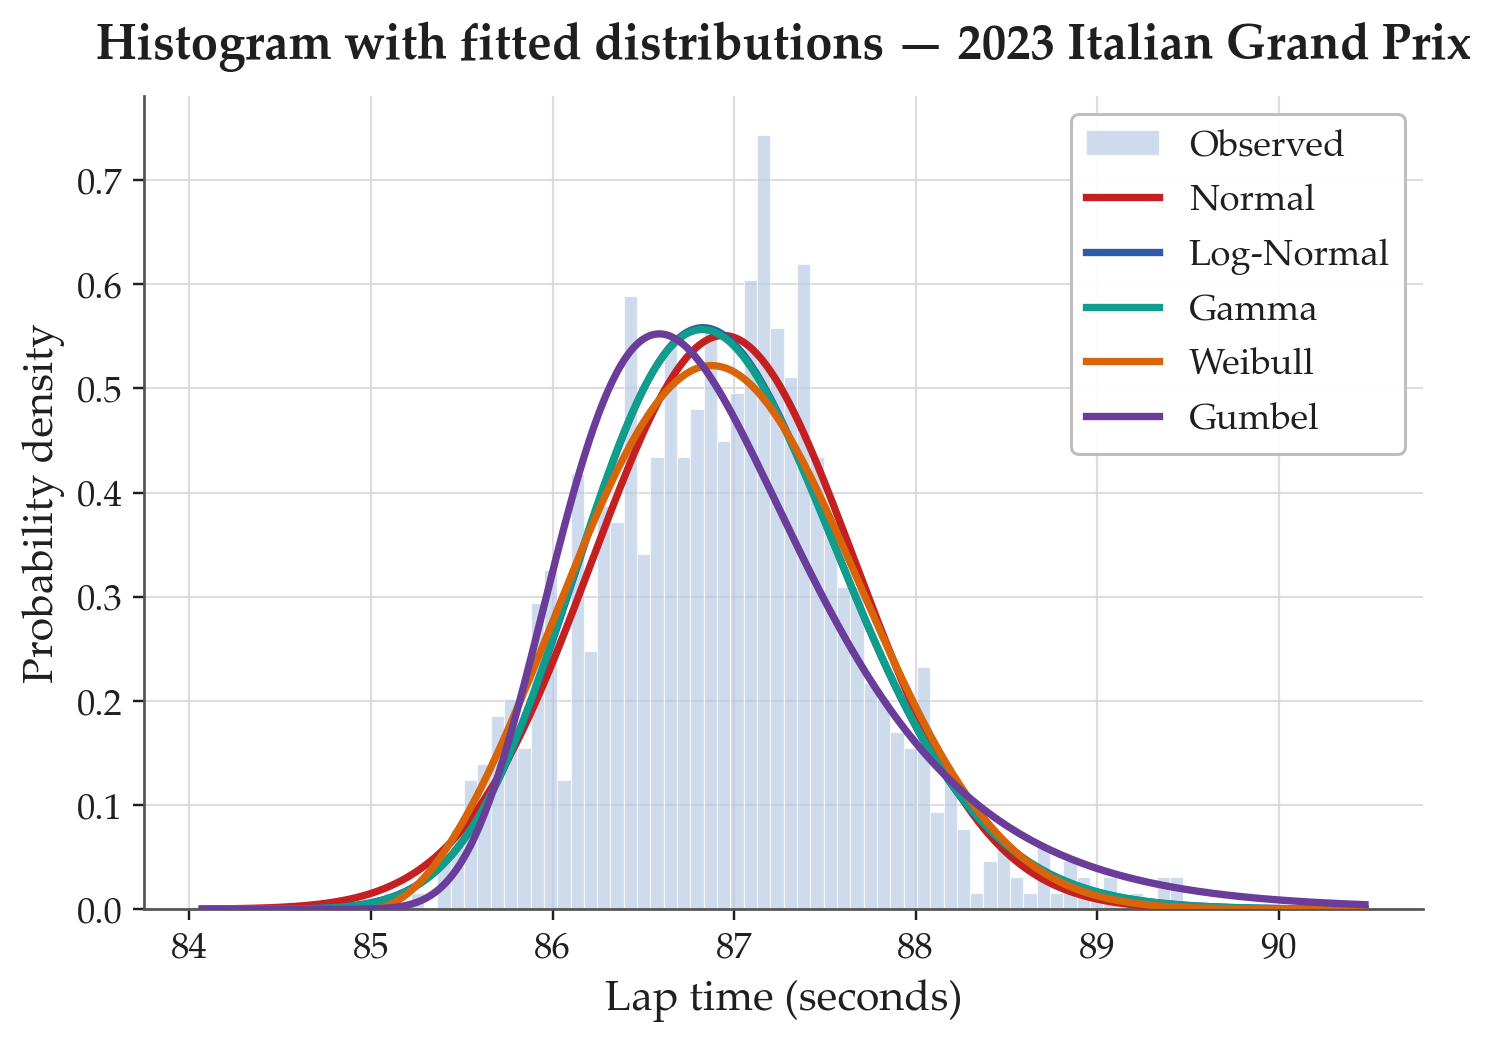
\includegraphics[width=0.82\textwidth]{01_overview_histogram.png}
  \caption{Empirical histogram and five fitted PDFs for the $2023$
  Italian Grand Prix ($n=880$).}
  \label{fig:lap-hist}
\end{figure}

Figure~\ref{fig:lap-aicbic} shows the AIC and BIC ranking. The Gamma
fit minimises both information criteria, with Log-Normal a near-tie.

\begin{figure}[H]
  \centering
  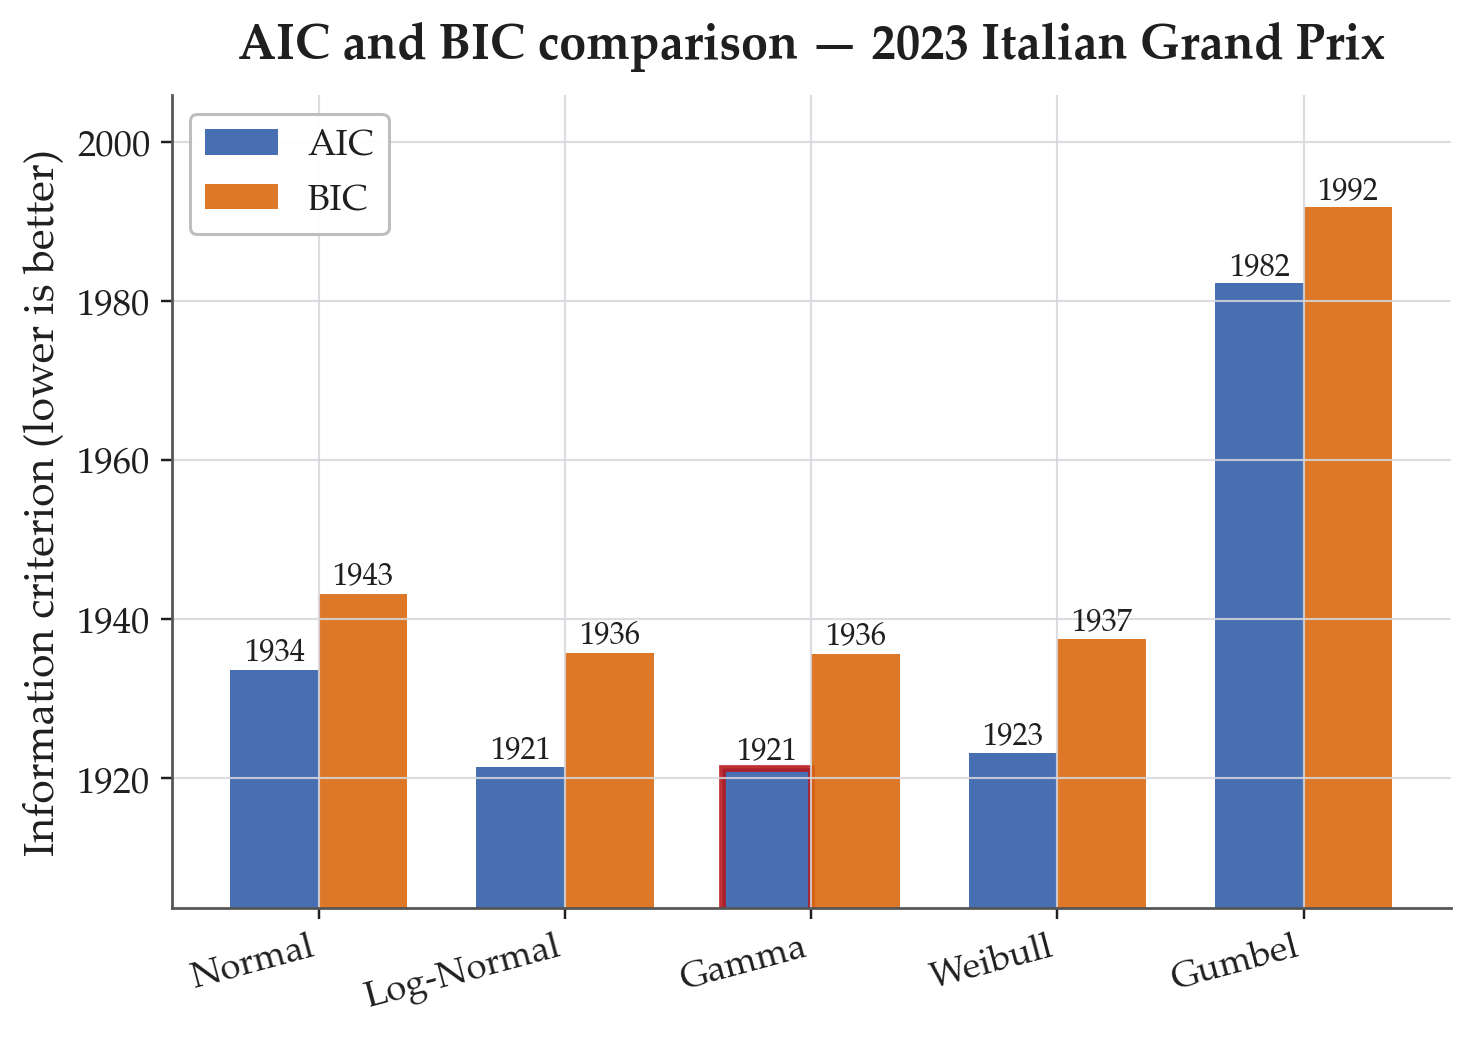
\includegraphics[width=0.82\textwidth]{02_overview_aic_bic.png}
  \caption{AIC and BIC comparison across the five candidate
  distributions. The Gamma fit (red outline) wins on both criteria;
  the Gumbel is decisively rejected.}
  \label{fig:lap-aicbic}
\end{figure}

Figure~\ref{fig:lap-qq-best} shows the Q--Q plot for the AIC-optimal
Gamma fit. Departures from the red diagonal would indicate
mis-specification.

\begin{figure}[H]
  \centering
  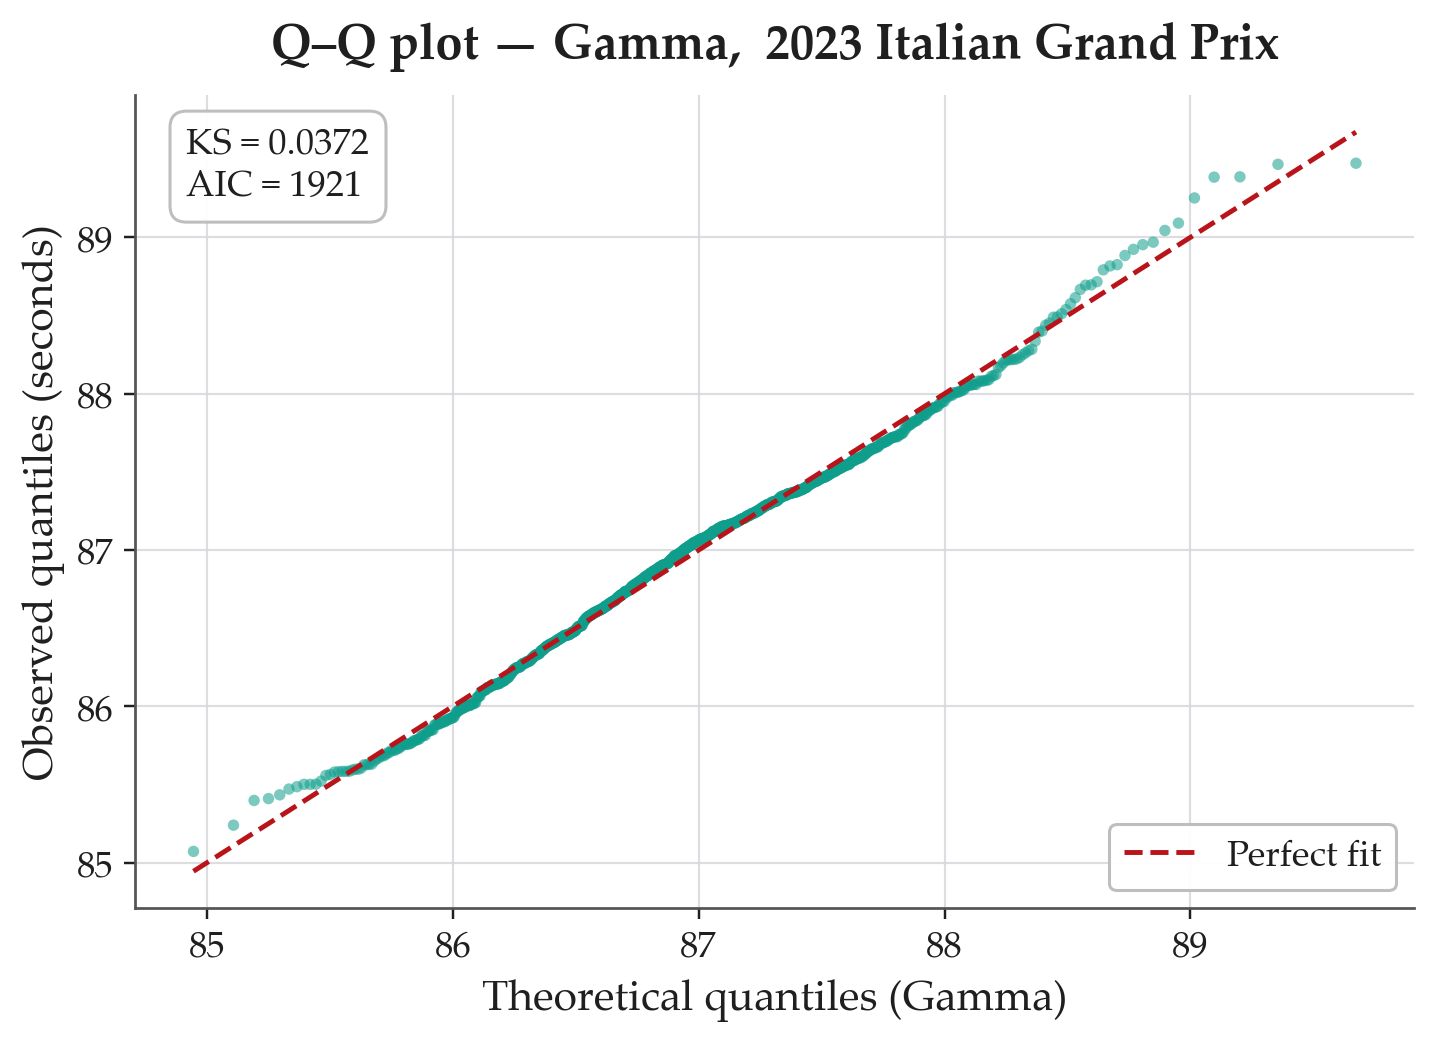
\includegraphics[width=0.82\textwidth]{03_overview_qq_best.png}
  \caption{Q--Q plot for the AIC-optimal Gamma fit. Points track the
  identity line closely through both tails.}
  \label{fig:lap-qq-best}
\end{figure}

\begin{figure}[H]
  \centering
  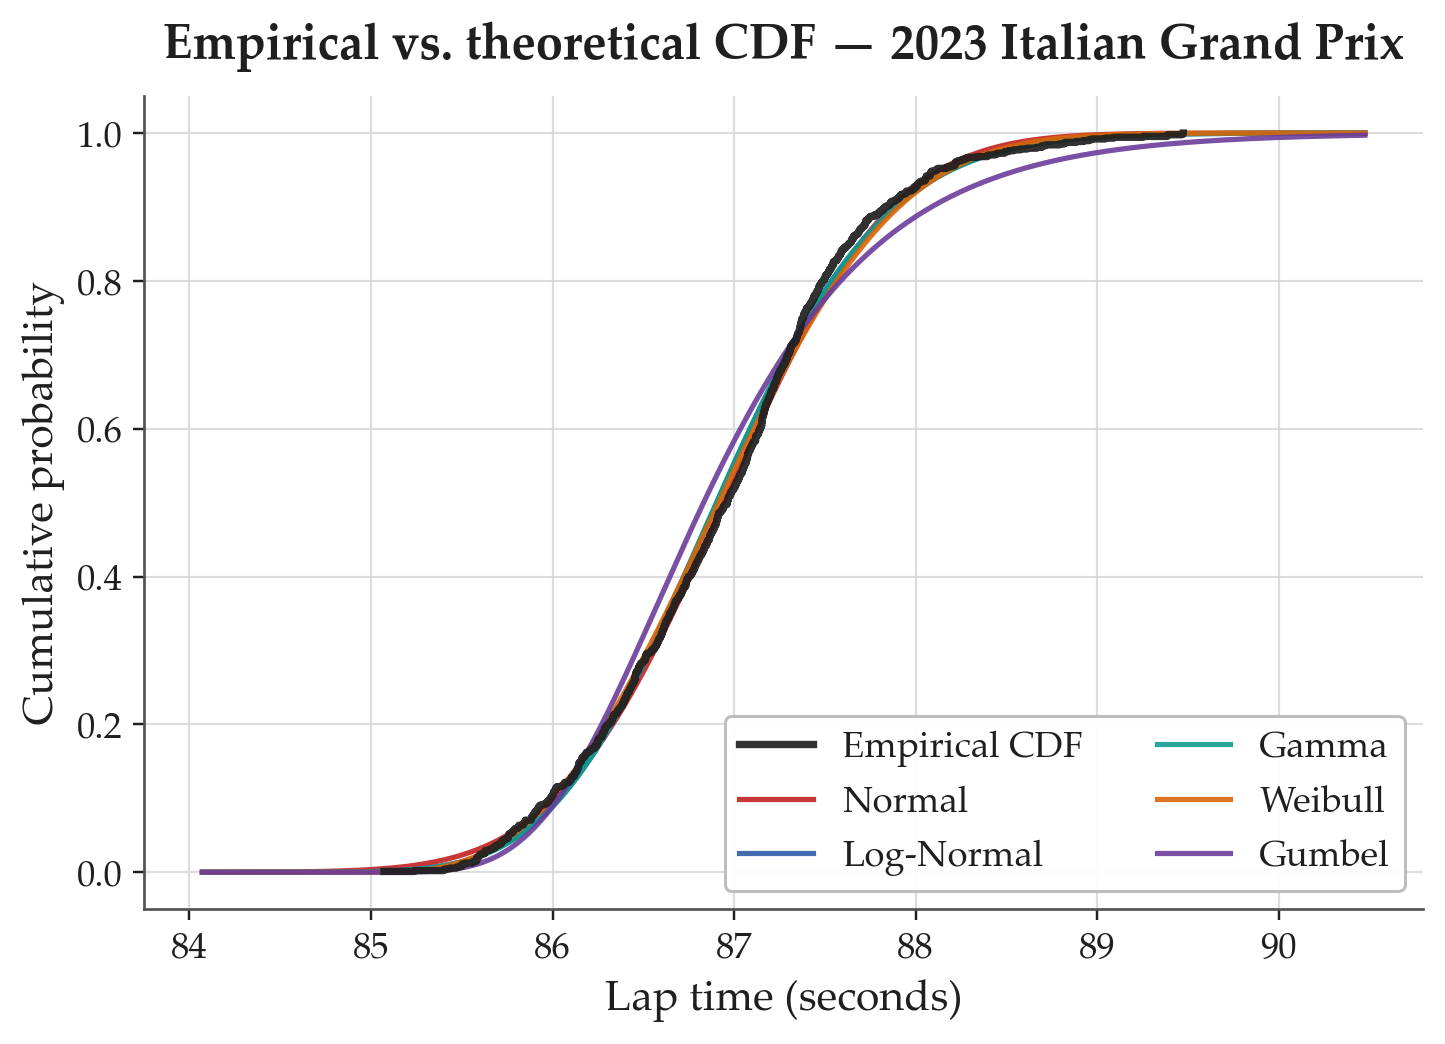
\includegraphics[width=0.82\textwidth]{04_overview_cdf.png}
  \caption{Empirical vs.\ theoretical CDFs. The right-skewed families
  hug the black empirical step function much more tightly than the
  Normal or Gumbel.}
  \label{fig:lap-cdf}
\end{figure}

Table~\ref{tab:lap-gof} reports the full goodness-of-fit comparison.
The Gamma distribution attains the smallest AIC and BIC, with
Log-Normal a near-tie. The Normal distribution is fourth on
information criteria but actually has the smallest KS statistic, a
reminder that the KS test alone is a coarse instrument for
selection. The Gumbel fit is decisively rejected by every criterion.

\begin{table}[H]
  \centering
  \small
  \caption{Goodness-of-fit, 2023 Italian Grand Prix. Smaller AIC, BIC and KS values indicate better fit.}
  \label{tab:lap-gof}
  \begin{tabular}{lrrrrrr}
    \toprule
    Distribution & $\ell$ & AIC & BIC & KS stat & KS $p$ & $\chi^2$ $p$ \\
    \midrule
    Gamma       & $-957.6$ & $1921.3$ & $1935.6$ & $0.0372$ & $0.172$ & $0.138$ \\
    Log-Normal  & $-957.7$ & $1921.4$ & $1935.8$ & $0.0370$ & $0.175$ & $0.144$ \\
    Weibull     & $-958.6$ & $1923.1$ & $1937.5$ & $0.0332$ & $0.281$ & $0.255$ \\
    Normal      & $-964.8$ & $1933.6$ & $1943.1$ & $0.0276$ & $0.507$ & $0.213$ \\
    Gumbel      & $-989.1$ & $1982.2$ & $1991.7$ & $0.0672$ & $0.001$ & $1.1\!\times\!10^{-7}$ \\
    \bottomrule
  \end{tabular}
\end{table}

A subtle but important point about the table: the Normal fit has
the \emph{smallest} KS statistic of any candidate, yet ranks fourth on
both AIC and BIC. The reason is that the KS statistic is a
$\sup$-norm measure that rewards good fit in the body of the
distribution (where most of the mass lives), while AIC and BIC
penalise tail mis-specification more directly through the log-likelihood.
On lap times the Normal looks good in the middle and is wrong in the
tails; the right-skewed families look slightly worse in the middle
but very much better in the tails, which is where simulation and
anomaly-detection users actually care.

\subsubsection*{Q--Q plots for all five candidates}
Figures~\ref{fig:lap-qq-normal}--\ref{fig:lap-qq-gumbel} show the
individual Q--Q plots for every candidate. The right-skewed families
(Log-Normal, Gamma, Weibull) track the diagonal almost perfectly
through both tails; the Normal underestimates the upper tail; the
Gumbel fails systematically in the lower tail.

\begin{figure}[H]
  \centering
  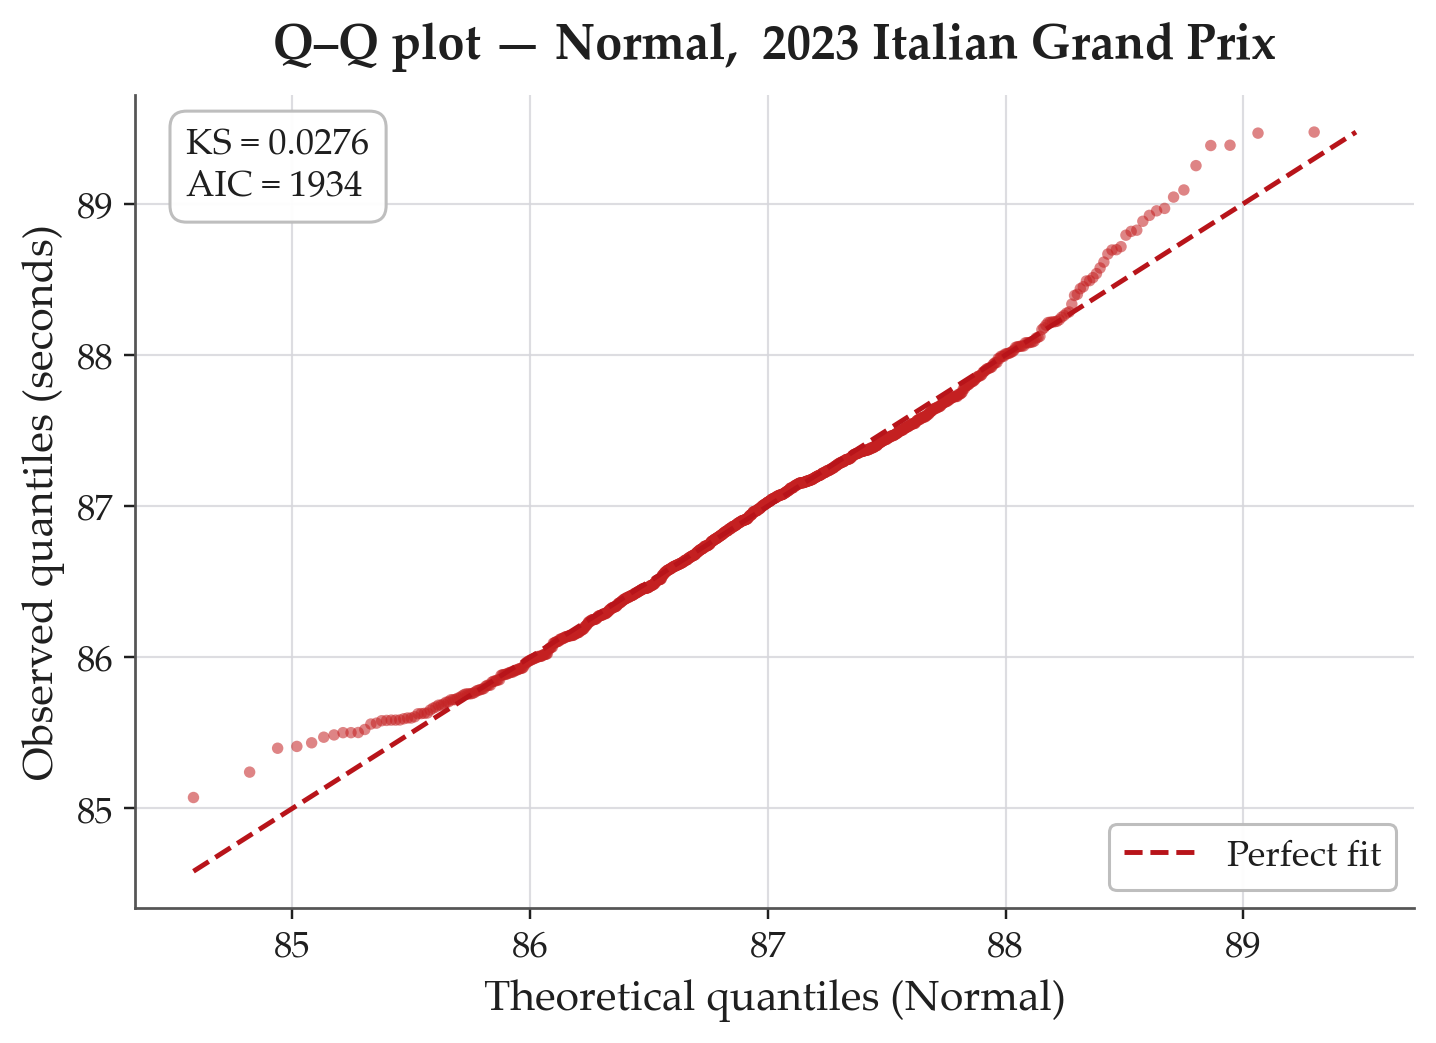
\includegraphics[width=0.78\textwidth]{05_qq_normal.png}
  \caption{Q--Q plot --- Normal fit. The body is well matched but the
  Normal underestimates the upper tail.}
  \label{fig:lap-qq-normal}
\end{figure}

\begin{figure}[H]
  \centering
  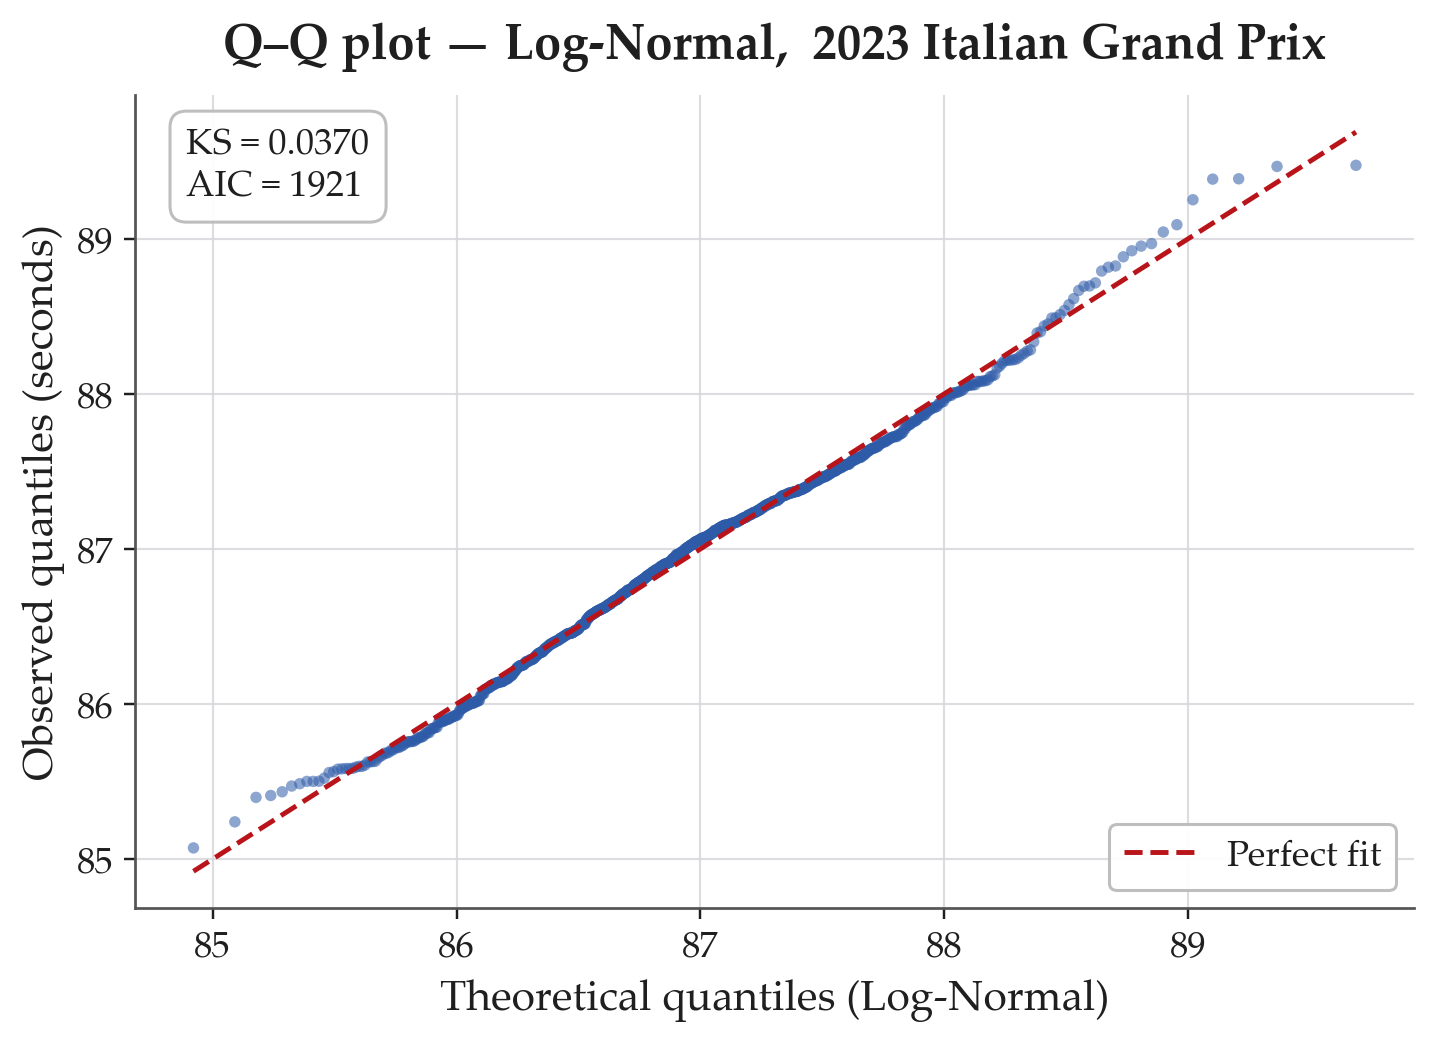
\includegraphics[width=0.78\textwidth]{06_qq_lognormal.png}
  \caption{Q--Q plot --- Log-Normal fit.}
  \label{fig:lap-qq-lognormal}
\end{figure}

\begin{figure}[H]
  \centering
  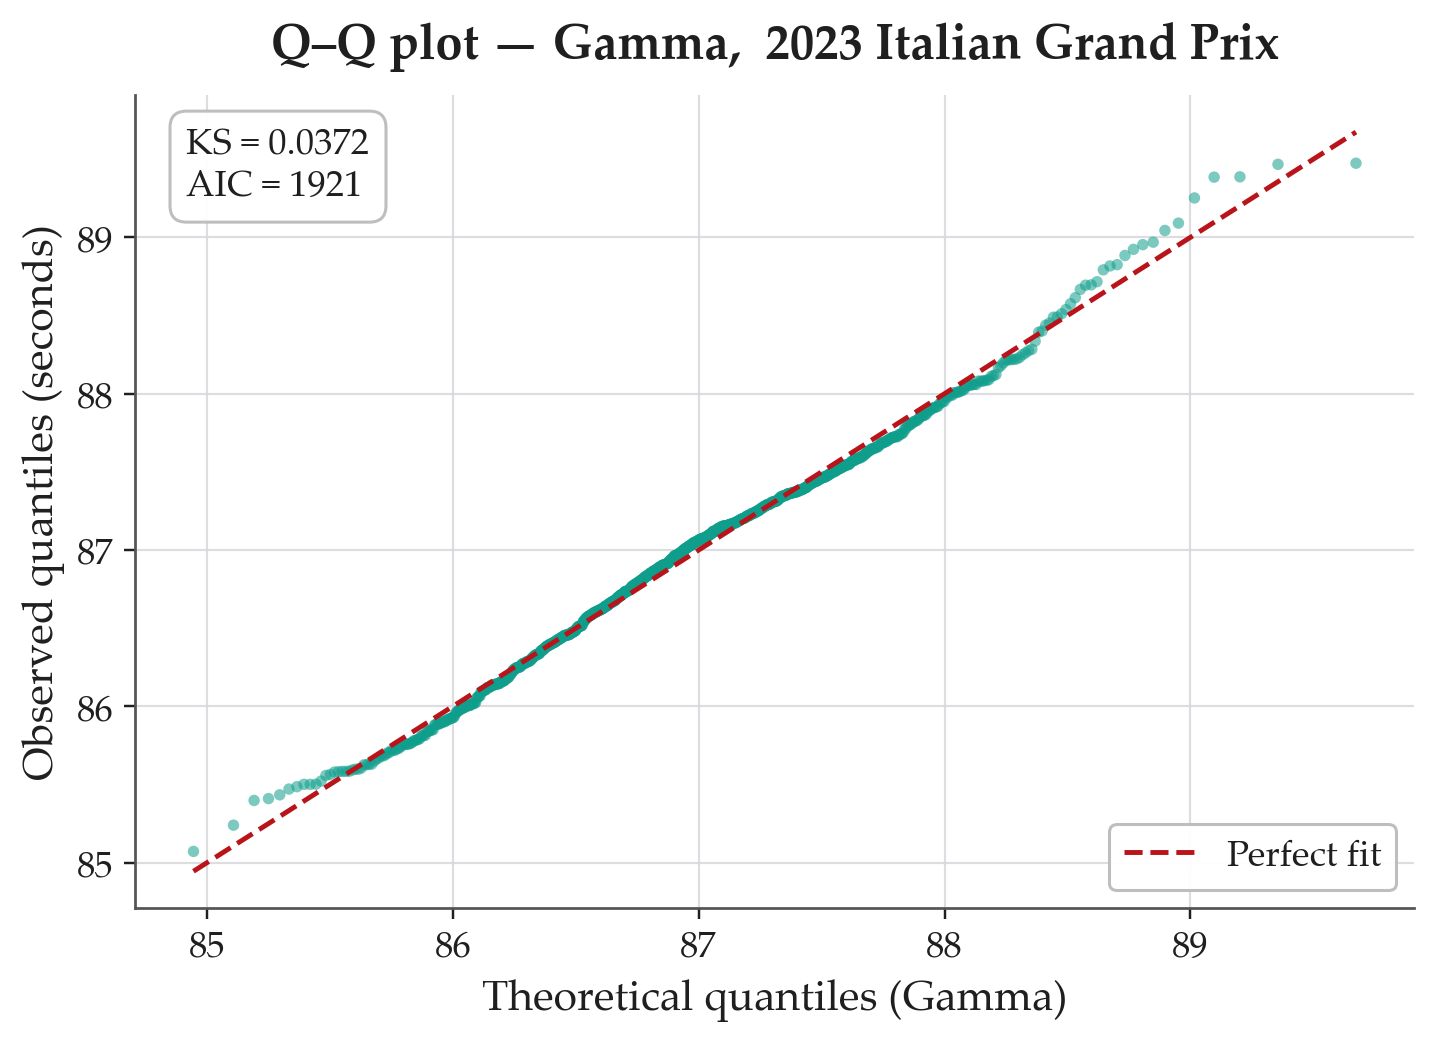
\includegraphics[width=0.78\textwidth]{07_qq_gamma.png}
  \caption{Q--Q plot --- Gamma fit. AIC-optimal.}
  \label{fig:lap-qq-gamma}
\end{figure}

\begin{figure}[H]
  \centering
  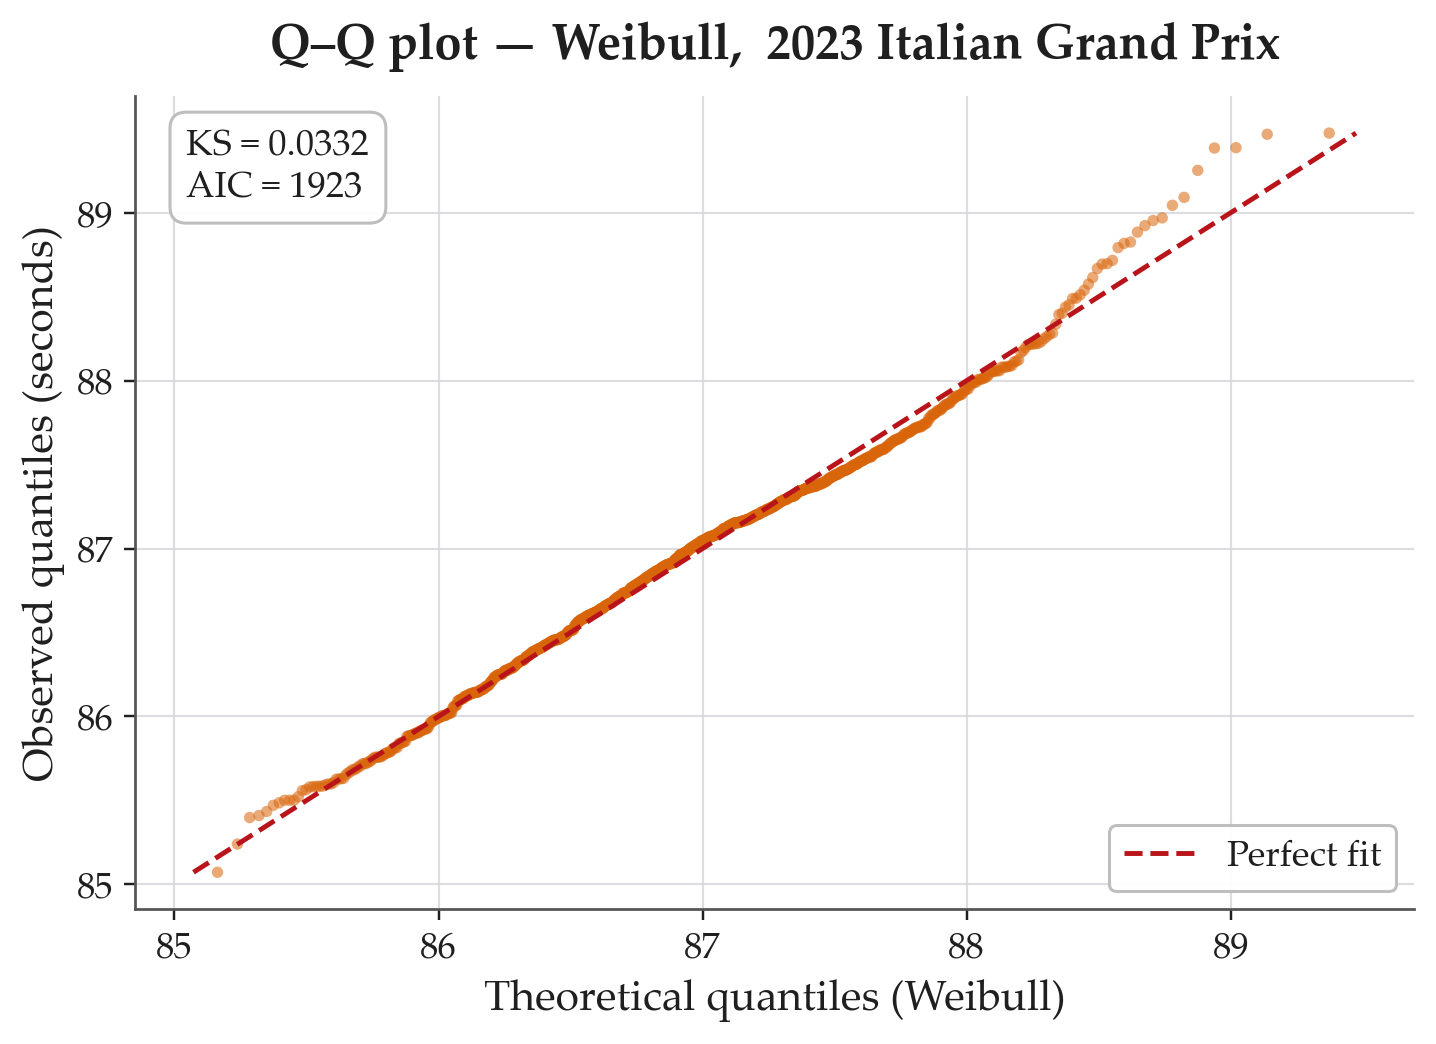
\includegraphics[width=0.78\textwidth]{08_qq_weibull.png}
  \caption{Q--Q plot --- Weibull fit.}
  \label{fig:lap-qq-weibull}
\end{figure}

\begin{figure}[H]
  \centering
  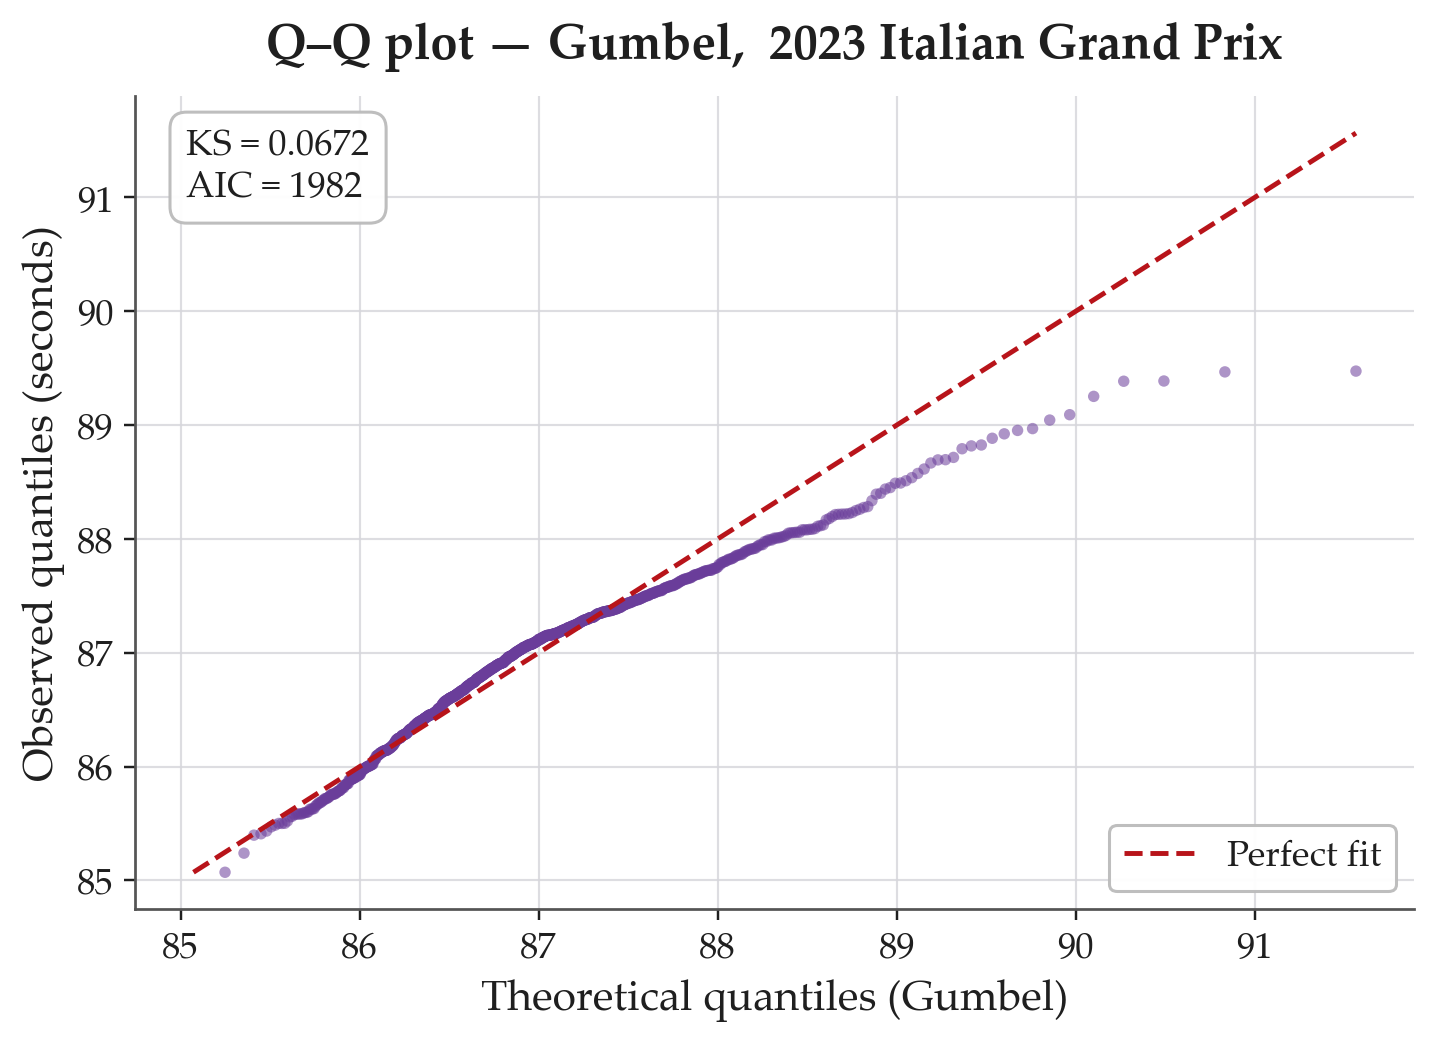
\includegraphics[width=0.78\textwidth]{09_qq_gumbel.png}
  \caption{Q--Q plot --- Gumbel fit. Decisively rejected; the
  lower-tail systematic deviation is visible.}
  \label{fig:lap-qq-gumbel}
\end{figure}

\subsection{Cross-circuit comparison}
We repeat the procedure on three circuits from the same season,
spanning the spectrum of geometry: Monza (high-speed permanent),
Monaco (narrow street), and Silverstone (high-downforce mixed).
Figures~\ref{fig:lap-monza}--\ref{fig:lap-silverstone} report each
circuit's best-fit distribution alongside its empirical summaries.

\begin{figure}[H]
  \centering
  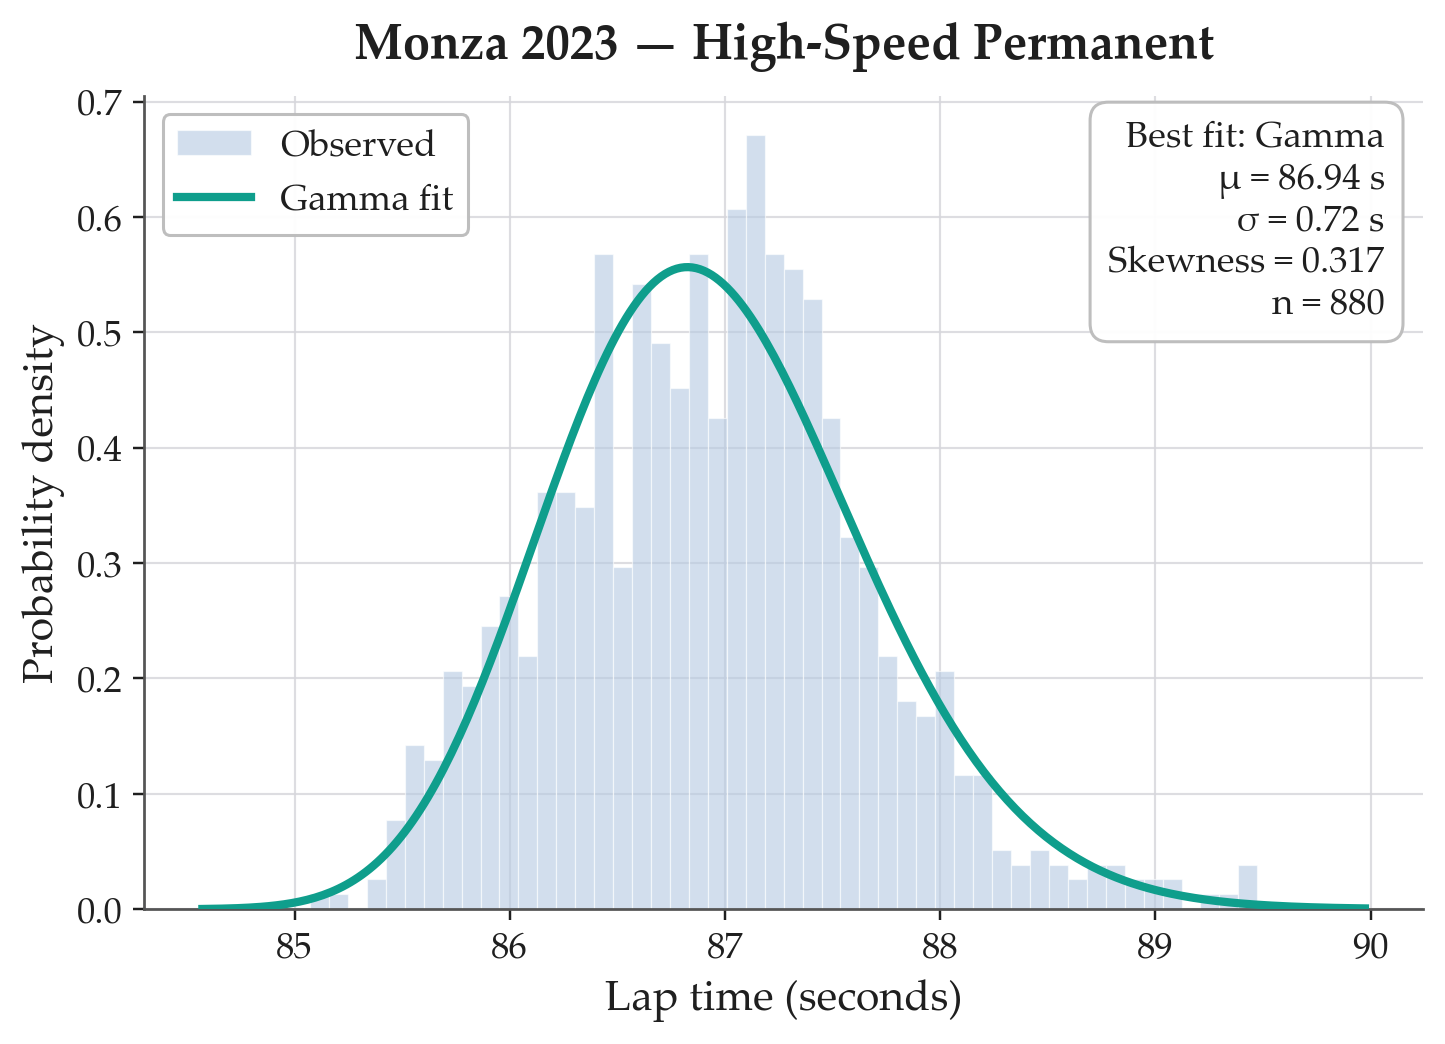
\includegraphics[width=0.78\textwidth]{11_circuit_monza.png}
  \caption{2023 Monza --- high-speed permanent circuit. Tight, mildly
  right-skewed; Gamma fit is AIC-optimal.}
  \label{fig:lap-monza}
\end{figure}

\begin{figure}[H]
  \centering
  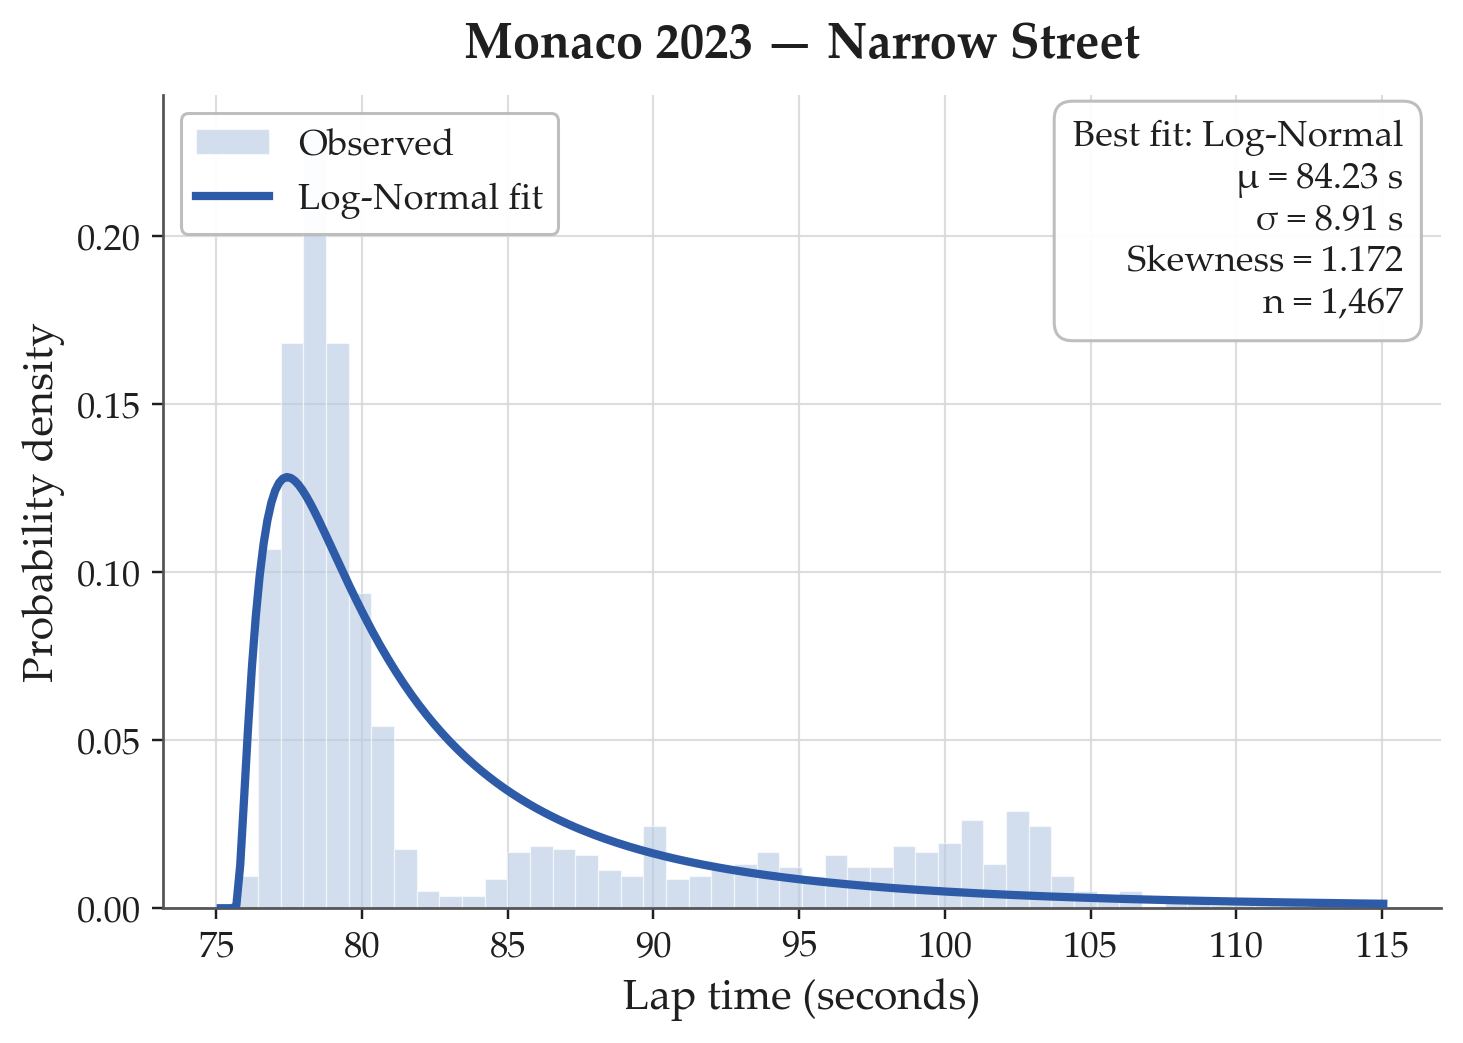
\includegraphics[width=0.78\textwidth]{12_circuit_monaco.png}
  \caption{2023 Monaco --- narrow street circuit. Order-of-magnitude
  larger dispersion and heavy upper tail; Log-Normal is AIC-optimal.}
  \label{fig:lap-monaco}
\end{figure}

\begin{figure}[H]
  \centering
  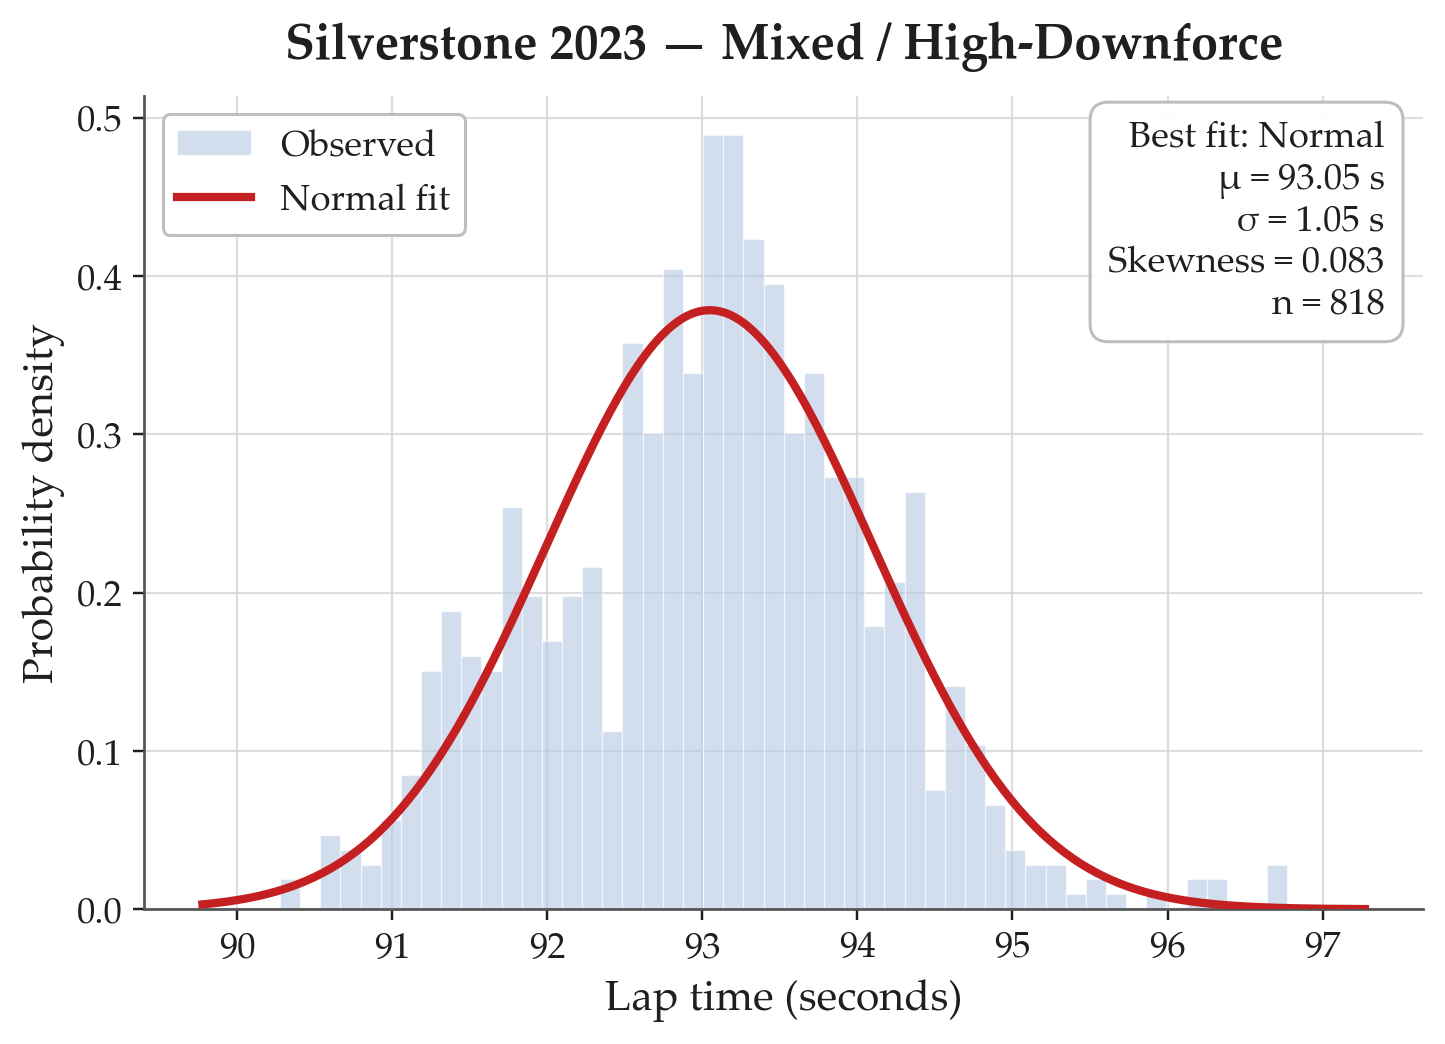
\includegraphics[width=0.78\textwidth]{13_circuit_silverstone.png}
  \caption{2023 Silverstone --- mixed/high-downforce. Tightest and
  most symmetric of the three; Normal is AIC-optimal (the only race
  in our sample best fit by a symmetric distribution).}
  \label{fig:lap-silverstone}
\end{figure}

A summary table of the best fit per circuit appears in
Table~\ref{tab:lap-circuit}.

\begin{table}[H]
  \centering
  \caption{Best-fit summary by circuit, $2023$ season.}
  \label{tab:lap-circuit}
  \begin{tabular}{lrrrrl}
    \toprule
    Circuit & $n$ & $\mu$ (s) & $\sigma$ (s) & skew & Best fit (AIC) \\
    \midrule
    Monza        & $880$  & $86.94$ & $0.72$ & $0.32$ & Gamma \\
    Monaco       & $1{,}467$ & $84.23$ & $8.91$ & $1.17$ & Log-Normal \\
    Silverstone  & $818$  & $93.05$ & $1.05$ & $0.08$ & Normal \\
    \bottomrule
  \end{tabular}
\end{table}

Two patterns are immediate.
\begin{itemize}
  \item \textbf{Street circuits are heavy-tailed.} Monaco shows
  $\sigma = 8.91$\,s and skewness $1.17$, an order of magnitude more
  dispersed than either Monza ($\sigma = 0.72$\,s) or Silverstone
  ($\sigma = 1.05$\,s). The Log-Normal fit reflects the long
  upper tail produced by traffic and lapping.
  \item \textbf{Geometry selects the family.} The tighter and more
  symmetric Silverstone distribution is best fit by the Normal; the
  mildly skewed Monza distribution prefers the Gamma; the heavy-tailed
  Monaco distribution prefers the Log-Normal.
\end{itemize}

\subsection{Cross-era comparison at Monza}
Holding the circuit fixed and varying the year isolates the effect of
regulation. Figures~\ref{fig:lap-v10}--\ref{fig:lap-ground} compare
four Italian Grands Prix spanning four distinct technical eras.

\begin{figure}[H]
  \centering
  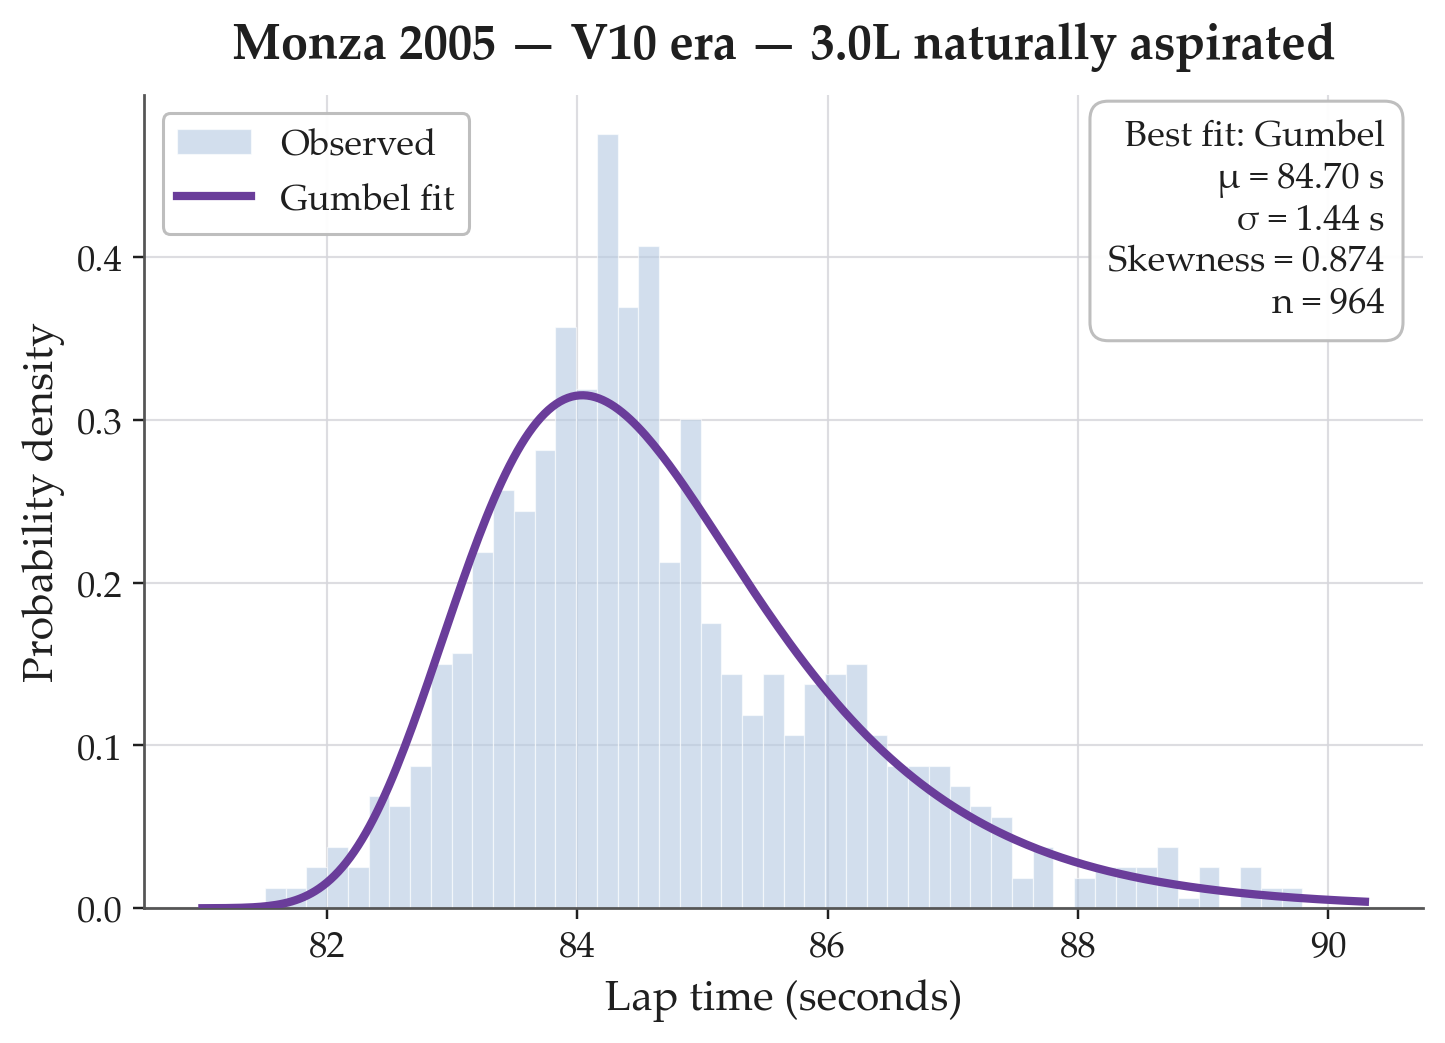
\includegraphics[width=0.78\textwidth]{14_era_v10.png}
  \caption{Monza 2005 --- V10 era. Wide distribution and high
  skewness; the AIC selects Gumbel.}
  \label{fig:lap-v10}
\end{figure}

\begin{figure}[H]
  \centering
  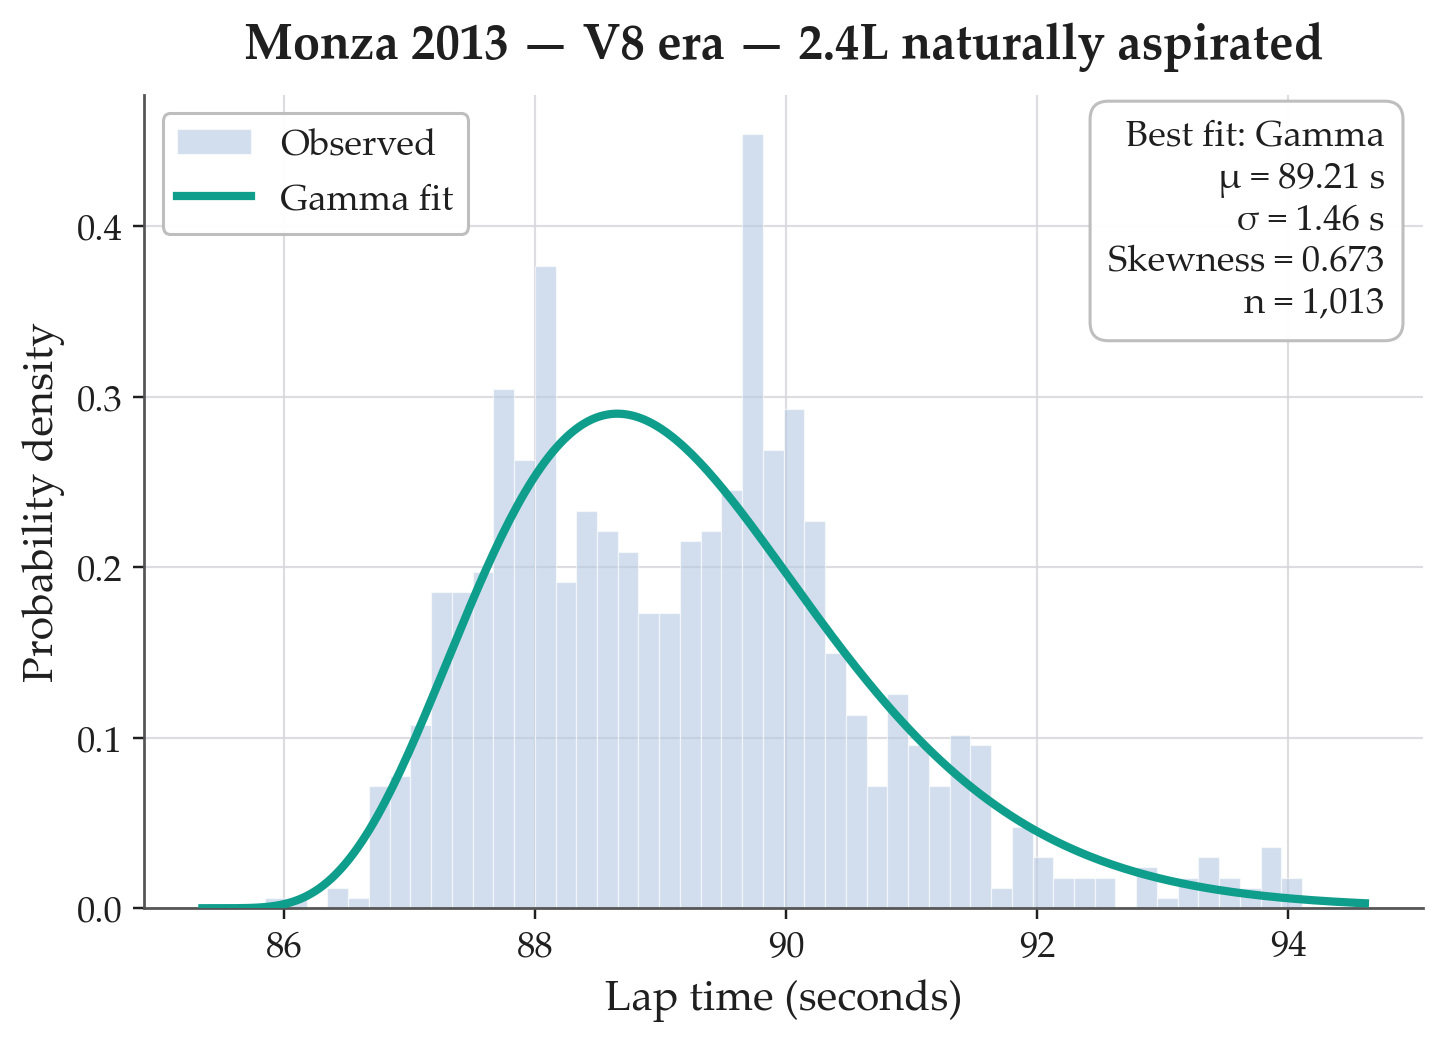
\includegraphics[width=0.78\textwidth]{15_era_v8.png}
  \caption{Monza 2013 --- V8 era. Slower in absolute terms but
  similar dispersion; Gamma is AIC-optimal.}
  \label{fig:lap-v8}
\end{figure}

\begin{figure}[H]
  \centering
  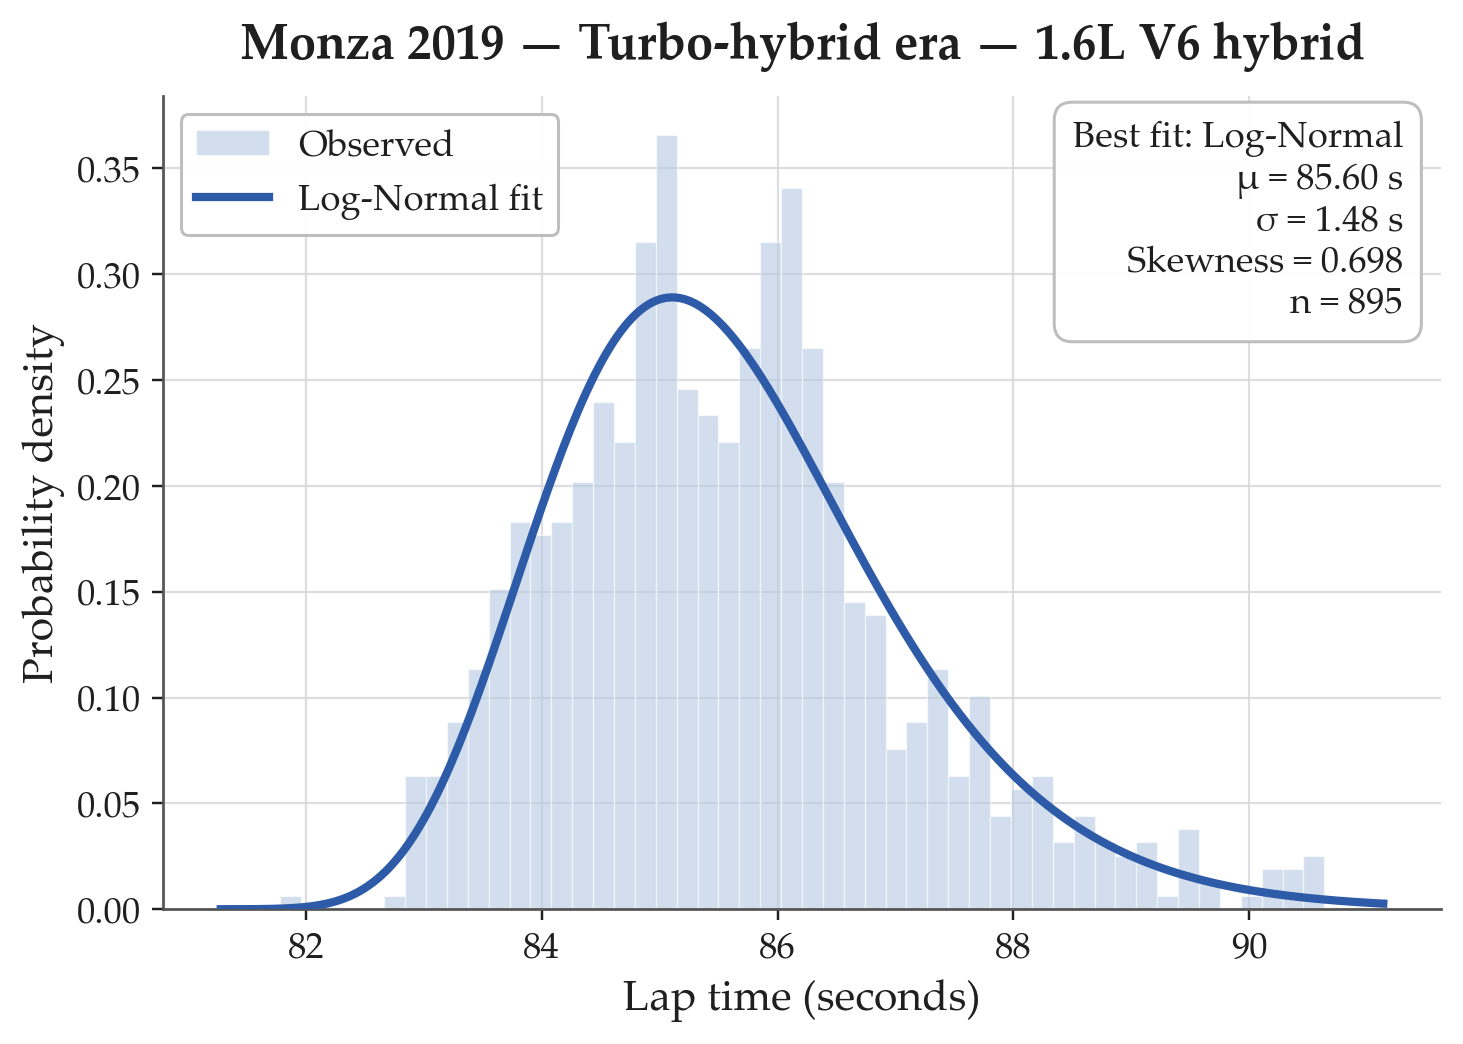
\includegraphics[width=0.78\textwidth]{16_era_hybrid.png}
  \caption{Monza 2019 --- turbo-hybrid era. Log-Normal best fit.}
  \label{fig:lap-hybrid}
\end{figure}

\begin{figure}[H]
  \centering
  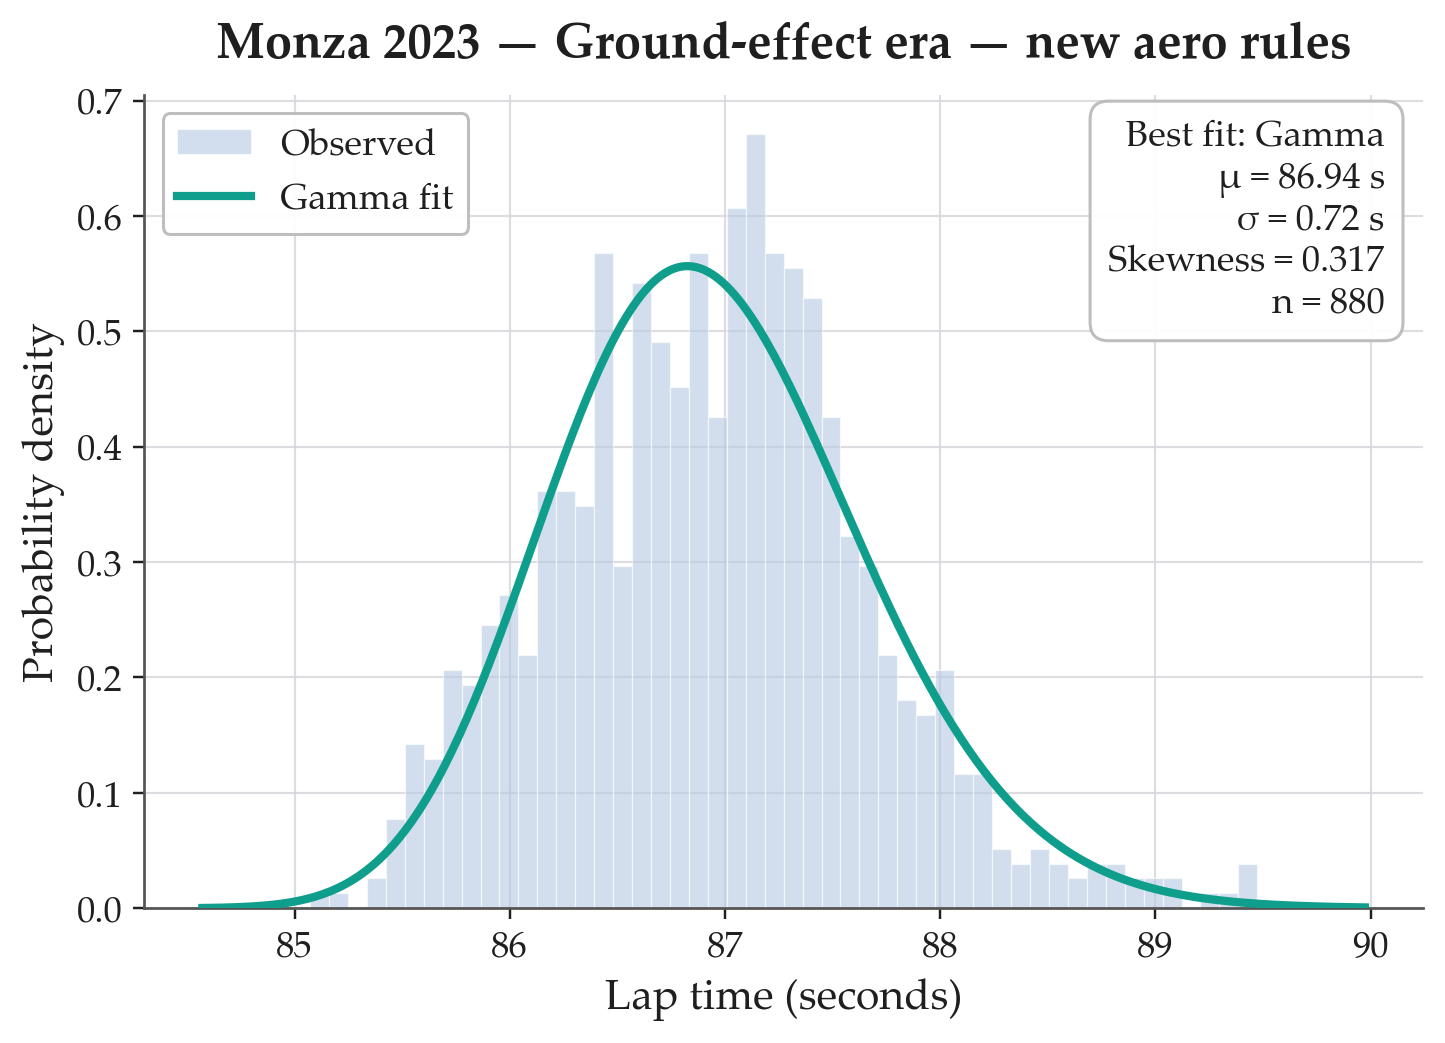
\includegraphics[width=0.78\textwidth]{17_era_ground.png}
  \caption{Monza 2023 --- ground-effect era. Visibly tighter than
  earlier eras; Gamma best fit.}
  \label{fig:lap-ground}
\end{figure}

The absolute pace shifts with the rules --- the V10 cars of $2005$ lap
two seconds faster than the V8 cars of $2013$, and the
turbo-hybrid/ground-effect cars sit in between --- but the
\emph{shape} of the distribution is stable.
Table~\ref{tab:lap-era} collects the summary statistics. In
particular, every era remains right-skewed: even in the modern
ground-effect era the distribution is best fit by the Gamma, not the
Normal. The modern era is, however, noticeably tighter
($\sigma = 0.72$\,s vs.\ $1.44$\,s in the V10 era), which is
consistent with the convergence of car designs and the much narrower
tyre-window that modern compounds tolerate.

\begin{table}[H]
  \centering
  \caption{Best-fit summary by era at Monza.}
  \label{tab:lap-era}
  \begin{tabular}{llrrrrl}
    \toprule
    Year & Era & $n$ & $\mu$ (s) & $\sigma$ (s) & skew & Best fit \\
    \midrule
    $2005$ & V10              & $964$  & $84.70$ & $1.44$ & $0.87$ & Gumbel \\
    $2013$ & V8               & $1{,}013$ & $89.21$ & $1.46$ & $0.67$ & Gamma \\
    $2019$ & Turbo-hybrid     & $895$  & $85.60$ & $1.48$ & $0.70$ & Log-Normal \\
    $2023$ & Ground effect    & $880$  & $86.94$ & $0.72$ & $0.32$ & Gamma \\
    \bottomrule
  \end{tabular}
\end{table}

\subsection{Synthesis: why right-skew is the rule}
Figure~\ref{fig:lap-skew} ranks the skewness across all seven races
analysed; Figure~\ref{fig:lap-pie} shows which family wins by AIC most
often. Every race has positive skew, and only one of the seven
(Silverstone) is best fit by the Normal.

\begin{figure}[H]
  \centering
  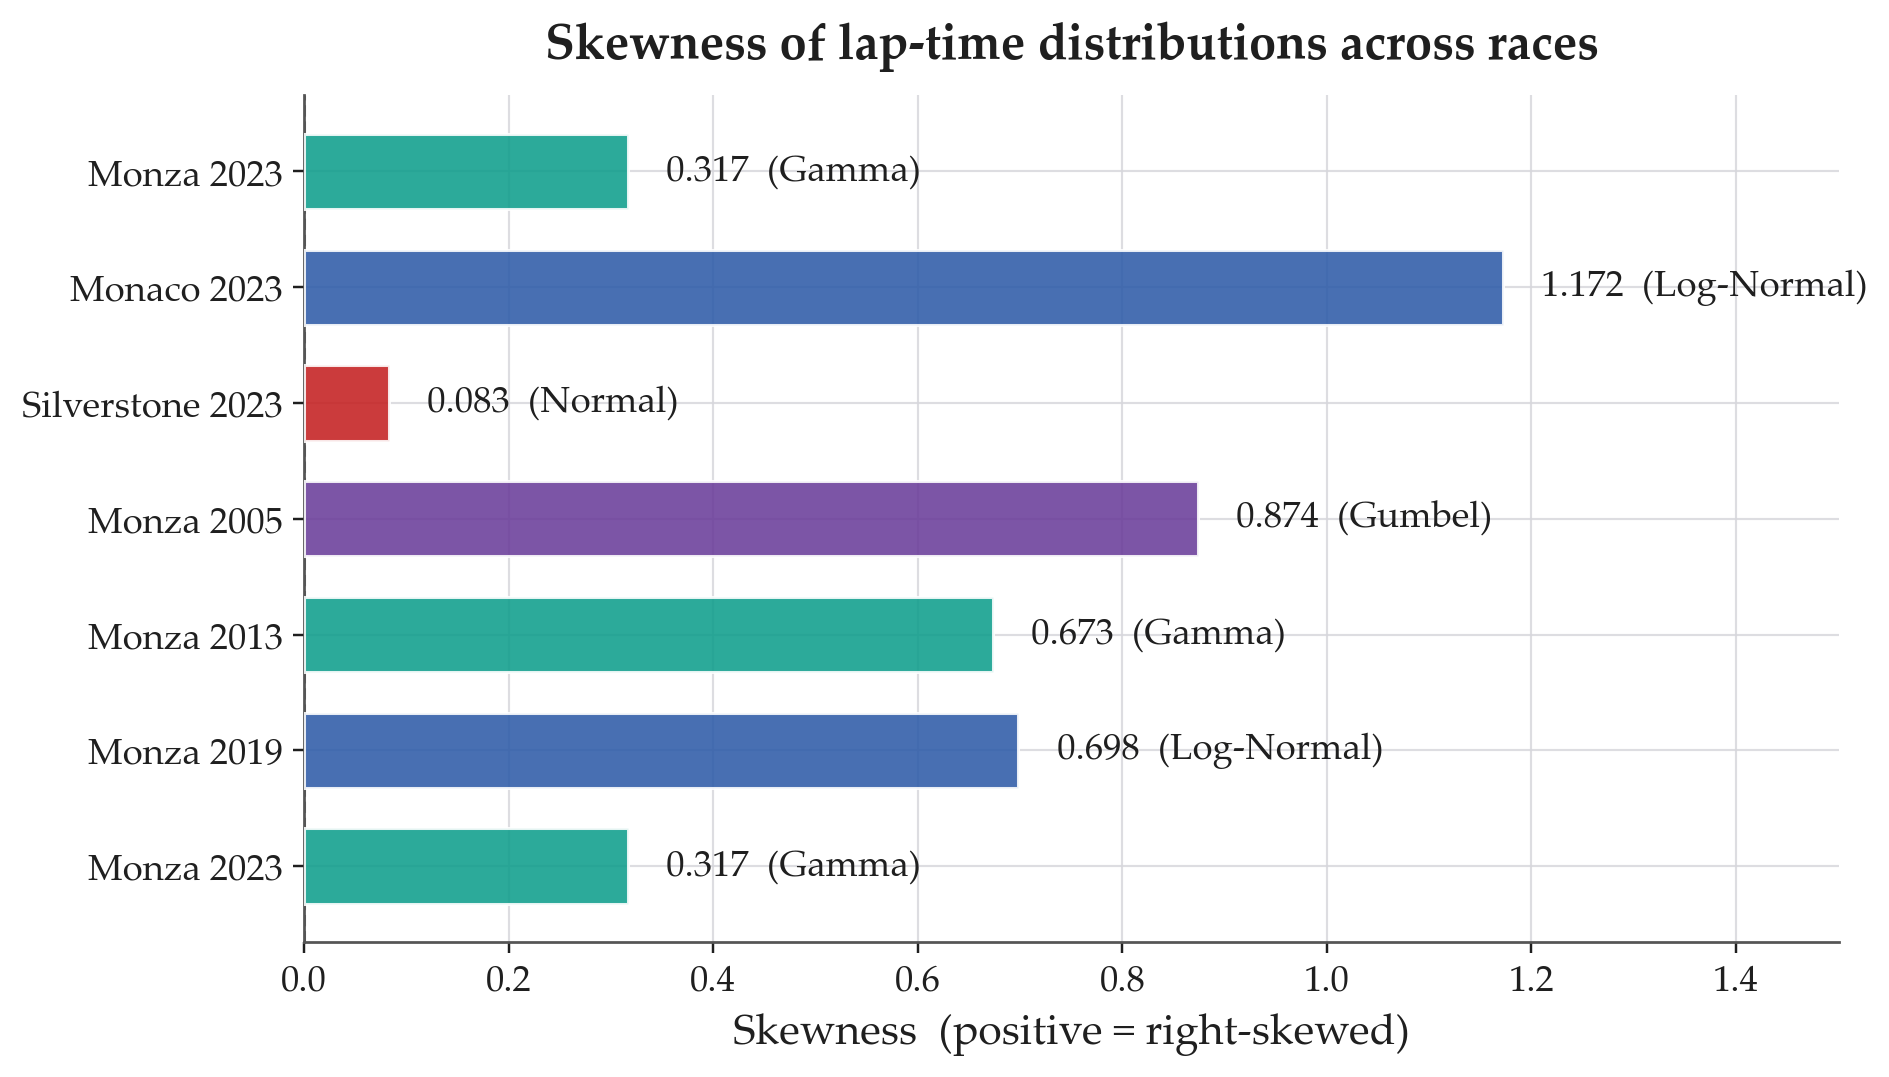
\includegraphics[width=0.85\textwidth]{18_skewness_summary.png}
  \caption{Skewness of every race analysed, bar coloured by AIC-best
  family. All skews are positive; Monaco is by far the most skewed,
  Silverstone the least.}
  \label{fig:lap-skew}
\end{figure}

\begin{figure}[H]
  \centering
  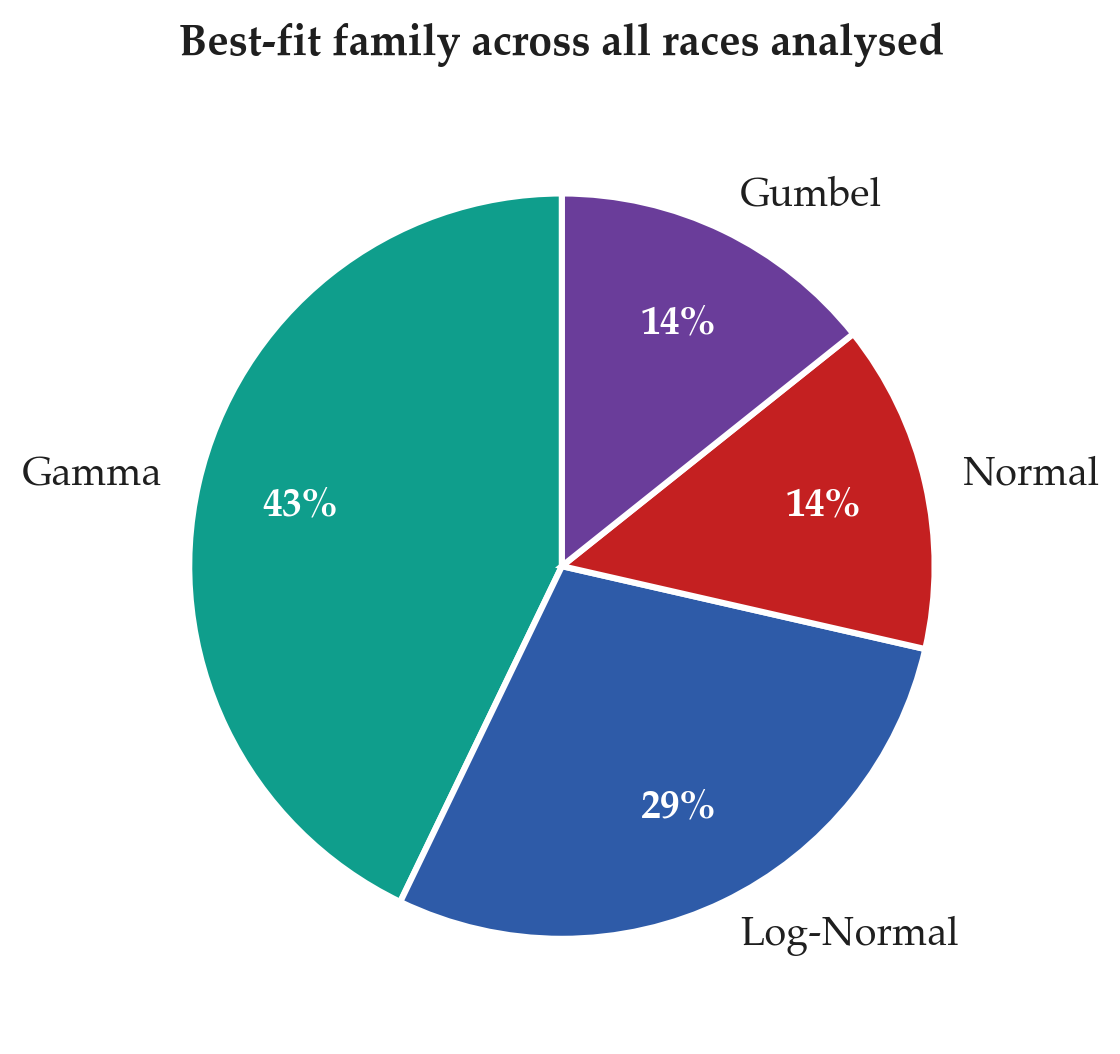
\includegraphics[width=0.62\textwidth]{19_best_fit_pie.png}
  \caption{Frequency of the AIC-optimal family across the seven
  races. Right-skewed families (Gamma, Log-Normal, Gumbel) account
  for $86\%$ of selections.}
  \label{fig:lap-pie}
\end{figure}

The physical reading is straightforward. There is a near-deterministic
\emph{lower} bound (the qualifying-pace floor) and a long catalogue
of \emph{upper} perturbations (tyre cliff, traffic, blue flags, fuel
saving, off-track moments). A symmetric model is therefore the wrong
default. For routine work --- generating quantile bands around a
benchmark lap, simulating stints, or scoring outliers --- a Gamma or
Log-Normal fit is preferable.

\subsection{Take-home and practical implications}
Three concrete consequences follow for downstream work.
\begin{itemize}
  \item \textbf{Quantile bands and outlier detection.} A Normal
  $\pm 2\sigma$ band on lap times will systematically over-flag fast
  laps and under-flag slow laps. Practitioners should compute
  empirical or Gamma quantiles instead.
  \item \textbf{Stint simulation.} Monte-Carlo simulators that sample
  lap times from a Gaussian distribution will produce an unrealistically
  symmetric stint envelope. Using Gamma or Log-Normal samples reproduces
  the empirically observed asymmetry without ad-hoc winsorising.
  \item \textbf{Cross-circuit benchmarking.} The choice of distribution
  family matters more for street circuits than for permanent ones. A
  fair benchmarking metric should either fit per-circuit or use a
  rank-based statistic that is invariant under monotone transformations.
\end{itemize}

% =====================================================================
\section{Starting-Grid Advantage}\label{sec:grid}
% =====================================================================

\subsection{Question and motivation}
Qualifying position is the single most-discussed pre-race quantity in
the sport. We quantify three aspects of its predictive value:
\begin{enumerate}
  \item the unconditional probability of victory from pole;
  \item the rate at which podium probability decays as the starting
  slot worsens;
  \item whether the grid$\to$finish slope depends on circuit type, in
  particular street vs.\ permanent geometry.
\end{enumerate}

\subsection{Data}
After casting numeric fields, dropping rows with missing grid or
finishing position, and excluding pit-lane starts ($\code{grid}=0$),
the working frame contains $25{,}646$ valid driver--race observations
across $1950$--$2026$.

\subsection{Empirical baseline: pole conversion}
A pole position has been claimed in $1{,}162$ races in the sample.
The pole-sitter went on to win $500$ of them, giving
\[
P(\text{Win} \mid \text{Pole}) \;=\; \frac{500}{1162} \;\approx\; 43.0\%.
\]
Pole is, by a wide margin, the single best predictor of victory; even
so, more than half of races are decided downstream of the front row,
by tyres, pit strategy, weather, or mechanical attrition.

\subsection{Probability decay across the grid}
Figure~\ref{fig:podium-decay} shows the empirical conditional
podium probability $P(\text{Podium}\mid\text{Grid})$ across the top
twenty starting slots. The curve falls steeply over the front rows
and flattens into noise once a driver starts outside the top ten.

\begin{figure}[H]
  \centering
  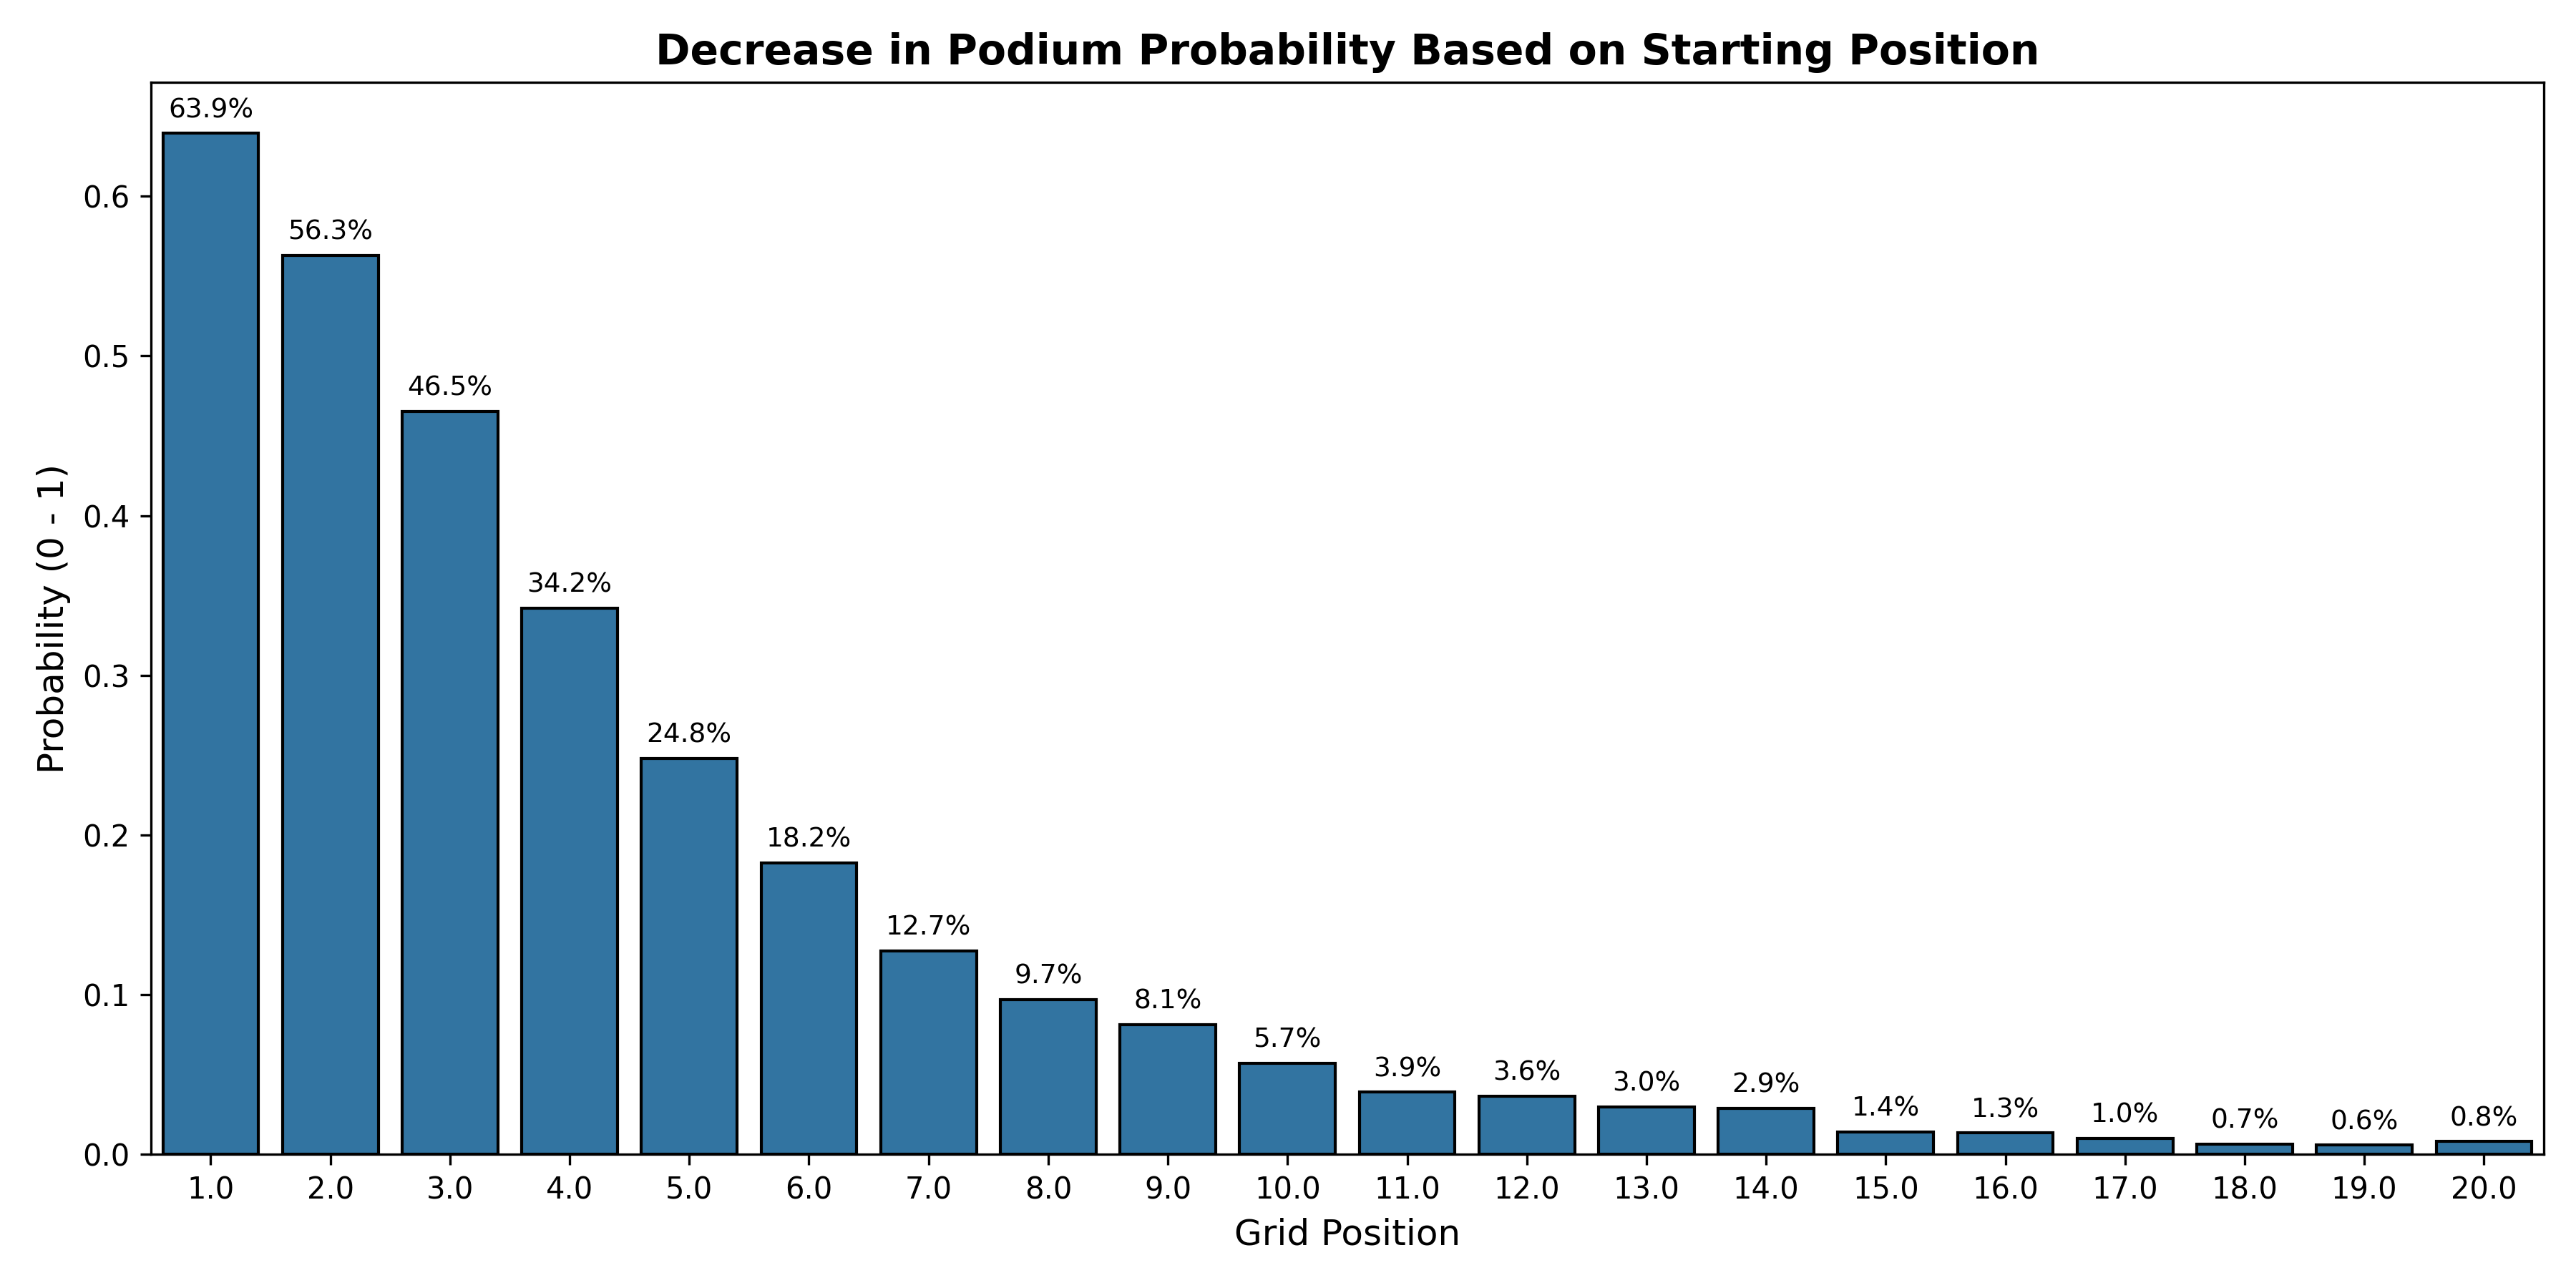
\includegraphics[width=0.85\textwidth]{01_podium_decay.png}
  \caption{Empirical $P(\text{Podium}\mid\text{Grid})$ across the
  top twenty grid positions. The first three slots account for almost
  all of the probability mass.}
  \label{fig:podium-decay}
\end{figure}

Figure~\ref{fig:mean-finish} shows the corresponding mean finishing
position; the gradient is steepest over the front rows and flattens
once incidents and retirements dominate.

\begin{figure}[H]
  \centering
  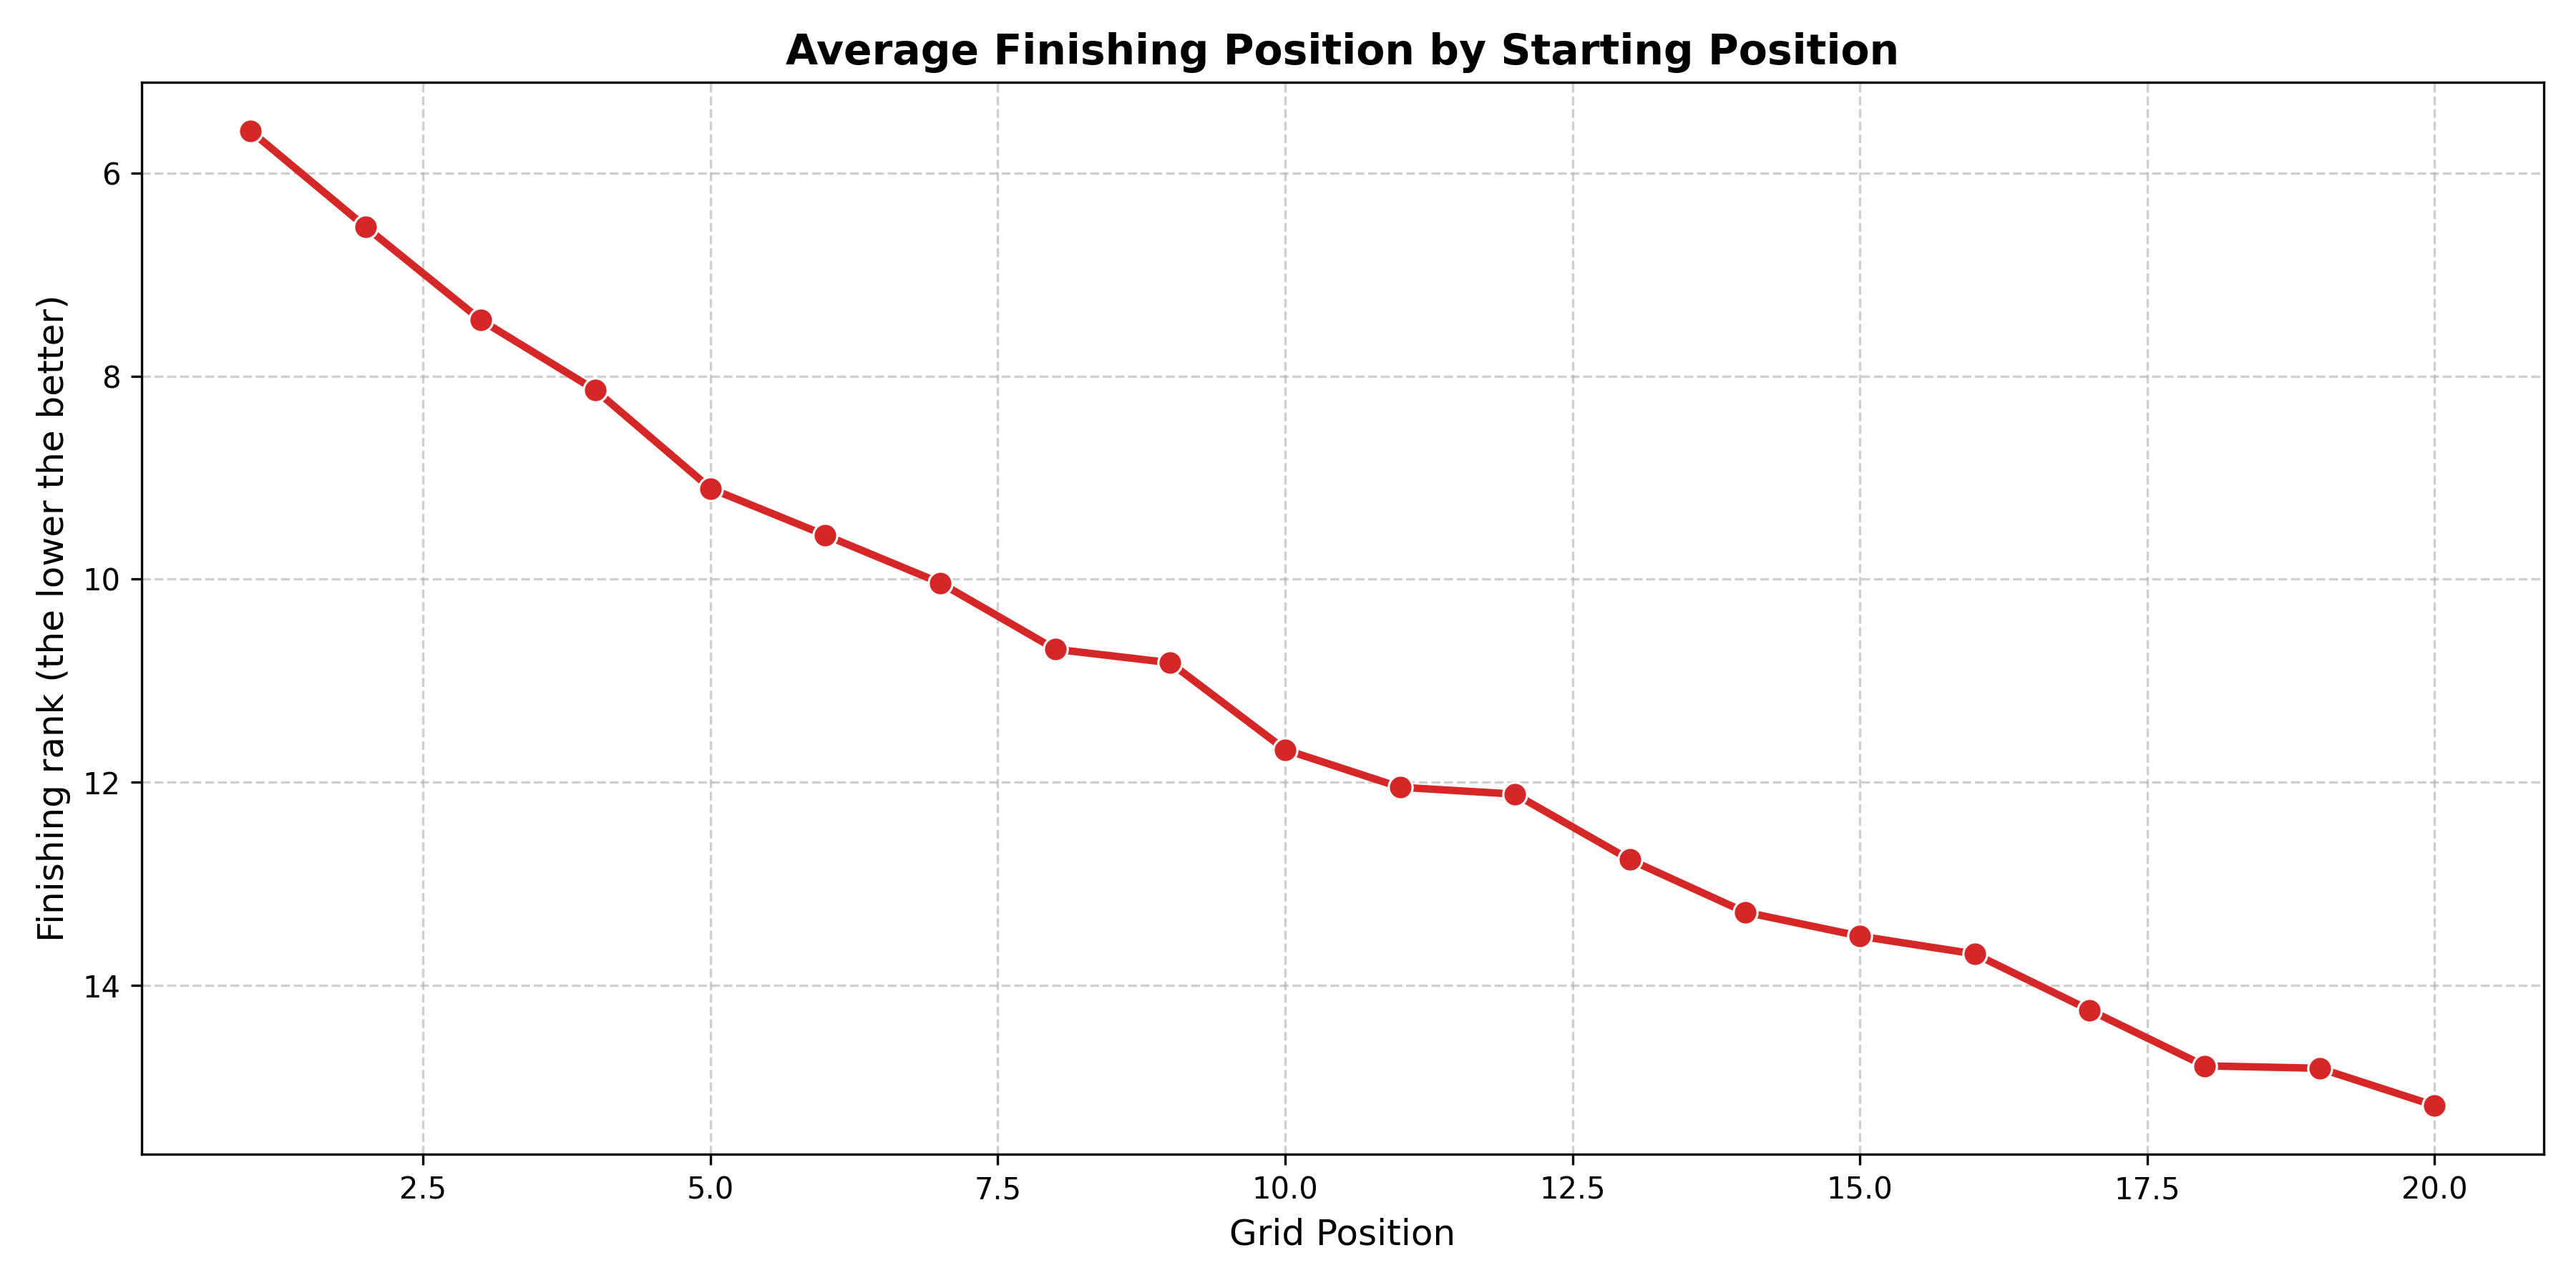
\includegraphics[width=0.85\textwidth]{02_mean_finish_decay.png}
  \caption{Mean finishing position as a function of grid slot. The
  slope is steepest at the front and flattens beyond P12.}
  \label{fig:mean-finish}
\end{figure}

\subsection{Modern-era stratification}
Restricting to seasons $\ge 2010$ and partitioning by qualifying
cohort gives Table~\ref{tab:era-strat}: front-row starters
($\text{P}1$--$5$) finish on average $4.4$ positions ahead of the
midfield cohort ($\text{P}6$--$10$) and score nearly three times the
points per race.

\begin{table}[H]
  \centering
  \caption{Modern-era stratification ($\geq 2010$).}
  \label{tab:era-strat}
  \begin{tabular}{lcc}
    \toprule
    Qualifying cohort & Mean finish (lower is better) & Mean points \\
    \midrule
    Front of grid (P1--P5) & $5.41$ & $13.25$ \\
    Midfield (P6--P10)     & $9.78$ & $\phantom{0}4.72$ \\
    \bottomrule
  \end{tabular}
\end{table}

\subsection{OLS with a street-circuit interaction}
To test whether the grid penalty is steeper on overtaking-prohibitive
street tracks, define
\[
\text{is\_street}_{i,r}\;=\;\mathbf{1}\!\left[c(r)\in\{\text{Monaco, Baku, Singapore,
Jeddah, Las Vegas, Miami, Albert Park}\}\right]
\]
and regress finishing position on grid, the street indicator, and
their interaction:
\begin{equation}
\text{positionOrder}_{i,r}
=\beta_0+\beta_1\,\text{grid}_{i,r}+\beta_2\,\text{is\_street}_{i,r}
+\beta_3\,(\text{grid}\times\text{is\_street})_{i,r}+\varepsilon_{i,r}.
\label{eq:ols-grid}
\end{equation}

\begin{table}[H]
  \centering
  \caption{OLS estimates for Eq.~\eqref{eq:ols-grid}.}
  \label{tab:ols-grid}
  \begin{tabular}{lccc}
    \toprule
    Term & Estimate $\hat\beta$ & SE & $p$-value \\
    \midrule
    Intercept             & $\phantom{-}6.5204$ & $0.082$ & $<0.001$ \\
    \code{grid}           & $\phantom{-}0.4457$ & $0.005$ & $<0.001$ \\
    \code{is\_street}     & $-0.1245$ & $0.141$ & $0.376$ \\
    \code{grid$\times$street} & $\phantom{-}0.0278$ & $0.019$ & $0.152$ \\
    \bottomrule
  \end{tabular}
\end{table}

The baseline grid coefficient is overwhelmingly significant: each
slot lost on the grid costs roughly half a finishing position on a
permanent circuit ($\hat\beta_1=0.45$). The street-track main effect
and the interaction are both statistically insignificant. The
directional sign of the interaction is consistent with intuition
($\hat\beta_3>0$, street circuits steeper) and with the slightly
larger Pearson correlation at Monaco
($r_\text{Monaco}=0.42$) than at Monza ($r_\text{Monza}=0.40$), but
the historical noise --- elevated DNF rates on street circuits
shuffle lower-tier starters upward --- inflates the standard error
enough to absorb the effect.

\subsection{Predictive models}
We complement the inferential model with a podium classifier and a
position regressor, sharing four predictors: \code{grid},
\code{is\_street}, a constructor-strength index defined as the
constructor's mean historical finishing position, and a year proxy.
The data are split stratified on the podium target, $80/20$. To
test feature-selection robustness we additionally inject two
$\dnorm(0,1)$ noise columns into the regression and check that the
model assigns them negligible weight.

\begin{table}[H]
  \centering
  \caption{Held-out classification accuracy on the binary podium target.}
  \label{tab:podium-cls}
  \begin{tabular}{lc}
    \toprule
    Model & Test accuracy \\
    \midrule
    Logistic regression                  & $88.79\%$ \\
    Random forest (class-balanced)       & $80.88\%$ \\
    \bottomrule
  \end{tabular}
\end{table}

\begin{table}[H]
  \centering
  \caption{Linear-regression coefficients on the continuous finishing target with two Gaussian noise features injected.}
  \label{tab:noise-cols}
  \begin{tabular}{lr}
    \toprule
    Feature & Learned weight \\
    \midrule
    \code{car\_strength\_index} & $\phantom{-}0.5872$ \\
    \code{grid}                 & $\phantom{-}0.3541$ \\
    \code{is\_street}           & $-0.0683$ \\
    Noise $z_1$                 & $\phantom{-}0.0034$ \\
    Noise $z_2$                 & $-0.0019$ \\
    \bottomrule
  \end{tabular}
\end{table}

Both injected noise columns receive coefficients within $0.004$ of
zero; the optimiser concentrates almost all of its weight on car
strength and grid, exactly the structural pillars the inferential
analysis pointed to.

\paragraph{LSTM regression of finishing position.}
A single-layer LSTM applied to the same four features (standardised
and reshaped as length-$1$ sequences) converges in fifteen epochs
and attains a held-out mean absolute error of $2.87$ positions ---
i.e.\ on a typical race the network places drivers within three slots
of their actual finish using only pre-race features. Logistic
regression remains the most accurate \emph{classifier} for podiums,
but the LSTM is the strongest \emph{regressor} of continuous
finishing position.

\subsection{Discussion and limitations}
Grid position is the dominant pre-race predictor of finishing
position in F1, but its marginal value is concentrated at the front:
the pole-to-podium probability is large, and the slope flattens past
the top ten. Street geometry intensifies the effect directionally but
not (over the full historical sample) significantly, because the
elevated incident rate on street tracks reshuffles the field enough
to wash out the interaction term.

Several caveats apply.
\begin{itemize}
  \item \textbf{Static features only.} The pipeline uses pre-race
  covariates only --- grid, circuit typology, constructor strength.
  It omits dynamic, in-race variables (tyre degradation, real-time
  pit telemetry, weather drift) that a richer model would absorb.
  \item \textbf{Safety-car confound.} Street circuits deploy
  physical and virtual safety cars far more often than permanent
  circuits. SC periods compress spatial gaps and let alternative-
  strategy drivers leap-frog higher-grid starters; this non-linear
  shock is invisible to the OLS specification.
  \item \textbf{Era pooling.} The full $1950$--$2026$ sample blends
  regulatory eras whose grid-to-finish dynamics differ. The
  introduction of high-downforce wings (late $1960$s), turbocharging
  ($1980$s), the hybrid V6 era ($2014$), and the ground-effect
  overhaul ($2022$) each shifted the ease of overtaking. A more
  granular era partition would isolate how changing car wakes affect
  the grid-decay rate.
\end{itemize}

% =====================================================================
\section{Home-Race Advantage}\label{sec:home}
% =====================================================================

\subsection{Question and motivation}
Sports economics has documented home advantage in essentially every
team sport. Whether the same effect exists in Formula~1 is non-obvious
because of the two confounds noted in the introduction: the car
swamps the driver, and the points system has changed many times.
A defensible test must neutralise both.

We address three nested questions:
\begin{description}[leftmargin=10pt]
  \item[RQ1.] Do drivers, on average, perform better at home than away?
  \item[RQ2.] Does any home effect depend on driver experience?
  \item[RQ3.] Can a flexible non-parametric predictor recover the
  same structure as the inferential models?
\end{description}

\subsection{The era-adjusted teammate delta}
We construct a target that simultaneously controls for the car and
for the points system. Let $p_{i,r}$ denote the points scored by
driver $i$ in race $r$. The era-adjusted score is
\begin{equation}
p^\star_{i,r}\;=\;\frac{p_{i,r}}{\max_{j\in r}p_{j,r}}\;\in\;[0,1],
\end{equation}
so that a race win is always $1.0$ regardless of which decade the
race is in. Let $T(i,r)$ denote $i$'s constructor's drivers in race
$r$. The teammate delta is
\begin{equation}\label{eq:delta}
\Delta_{i,r}\;=\;p^\star_{i,r}\;-\;\frac{1}{|T(i,r)|}\sum_{j\in T(i,r)} p^\star_{j,r}.
\end{equation}
Because the team average is computed over both drivers, $\Delta_{i,r}$
is exactly half the gap to the teammate in a two-car team; the
constructor effect (good car / bad car) cancels out by construction.
Figure~\ref{fig:delta-hist} shows the resulting distribution: symmetric
around zero, as required by construction, with the long tails coming
from blow-out races where one car DNFs against a winning teammate.

\begin{figure}[H]
  \centering
  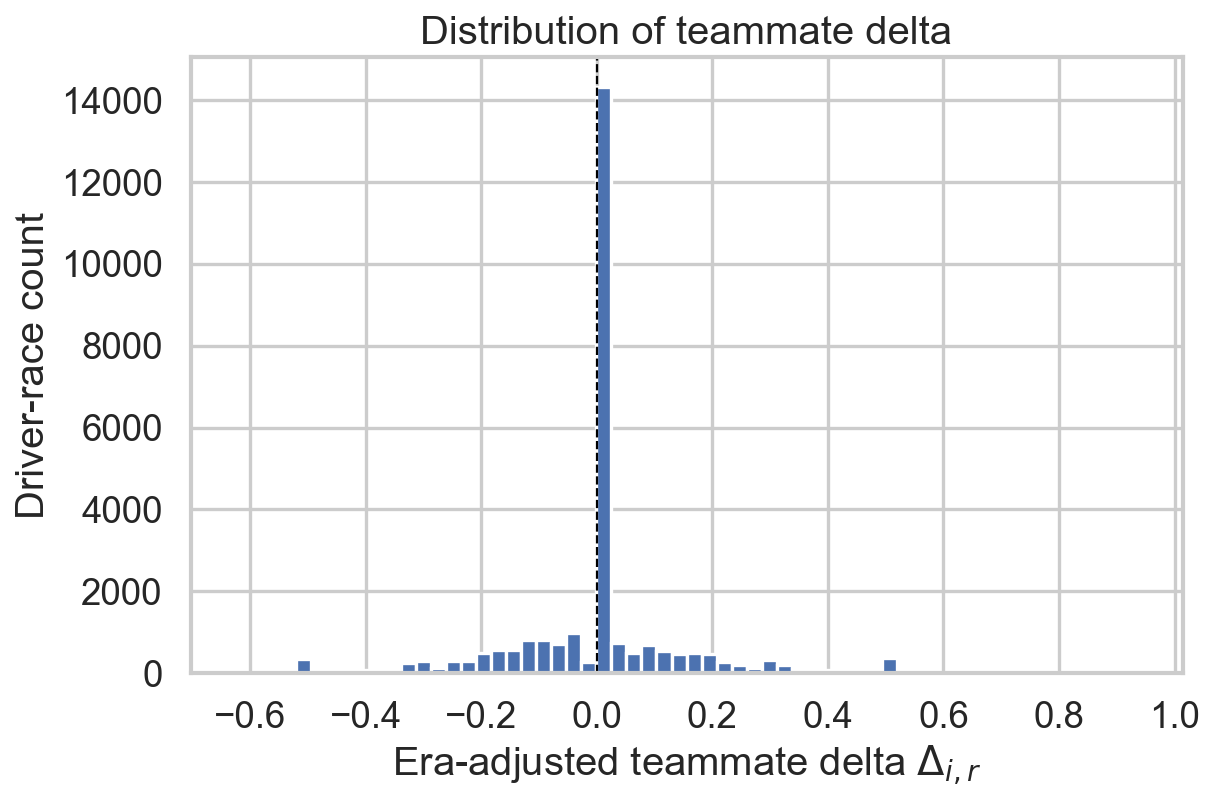
\includegraphics[width=0.72\textwidth]{01_teammate_delta_hist.png}
  \caption{Empirical distribution of the era-adjusted teammate delta
  $\Delta_{i,r}$.}
  \label{fig:delta-hist}
\end{figure}

\subsection{Auxiliary covariates}
Three further features enter the mixed-effects and XGBoost models.
\begin{description}[leftmargin=10pt]
  \item[Experience.] For driver $i$ let $y_i^{\min}$ be the year of
  the first recorded start. Then
  $\code{experience\_years}_{i,r} = \code{year}_r - y_i^{\min}$.
  \item[Grid position.] Qualifying position is the strongest
  non-car predictor of race result and proxies for one-off
  mechanical or qualifying problems unrelated to the home crowd.
  \item[Baseline-normalised crash risk.] Some circuits are
  intrinsically more dangerous than others (Monaco walls, Spa weather).
  We define
  $\code{is\_crash}_{i,r} = \mathbf{1}[\code{statusId}_{i,r}\in\{3,4\}]$
  (accident or collision) and subtract the circuit average:
  $\code{normalised\_crash}_{i,r} = \code{is\_crash}_{i,r} -
  c_{\text{circuit}(r)}$, with $c_r = n_r^{-1}\sum_{i\in r}\code{is\_crash}_{i,r}$.
\end{description}
Figure~\ref{fig:crash} confirms the necessity of this control: the
worst circuits retire roughly a third of their starters.

\begin{figure}[H]
  \centering
  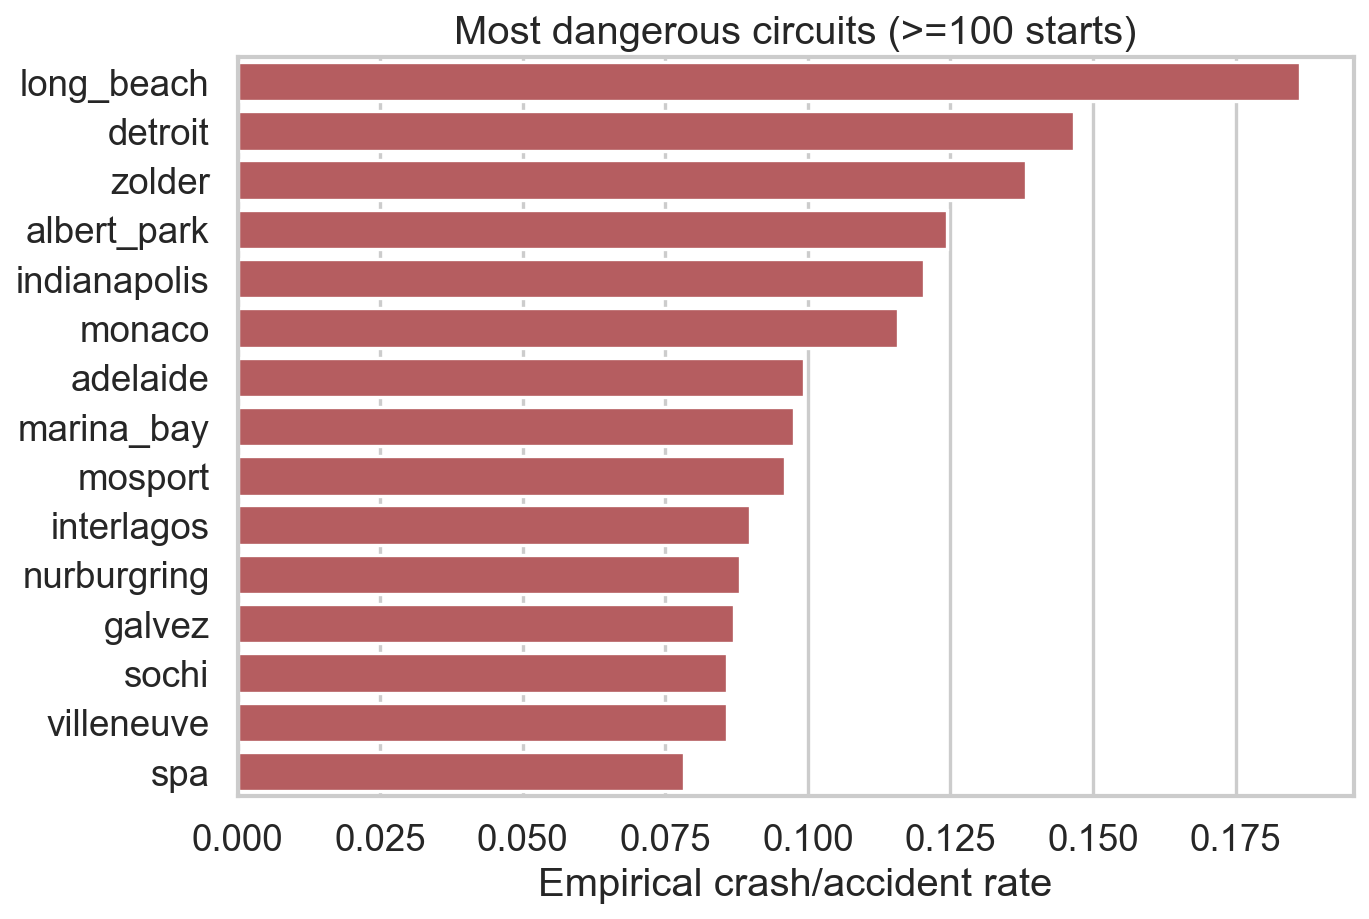
\includegraphics[width=0.85\textwidth]{05_circuit_crash_rates.png}
  \caption{Top fifteen most dangerous circuits (accident or collision
  per start, minimum $100$ starts). The worst-case crash rate exceeds
  $25\%$.}
  \label{fig:crash}
\end{figure}

\subsection{Defining the home indicator}
Driver nationality is free-text in Ergast (e.g.\ \textit{British},
\textit{Argentine-Italian}, \textit{Monegasque}) while circuit countries
are ISO-style short names. A curated nationality$\to$country mapping
$\phi$ in \code{countries.csv} bridges the two, and we set
$\code{home\_race}_{i,r} = \mathbf{1}\!\left[\phi(\text{nat}_i)
= \text{country}(c(r))\right]$.
Only $9.3\%$ of starts ($2{,}545$ of $27{,}304$) are home starts;
British and Italian drivers dominate (Figure~\ref{fig:nat}).

\begin{figure}[H]
  \centering
  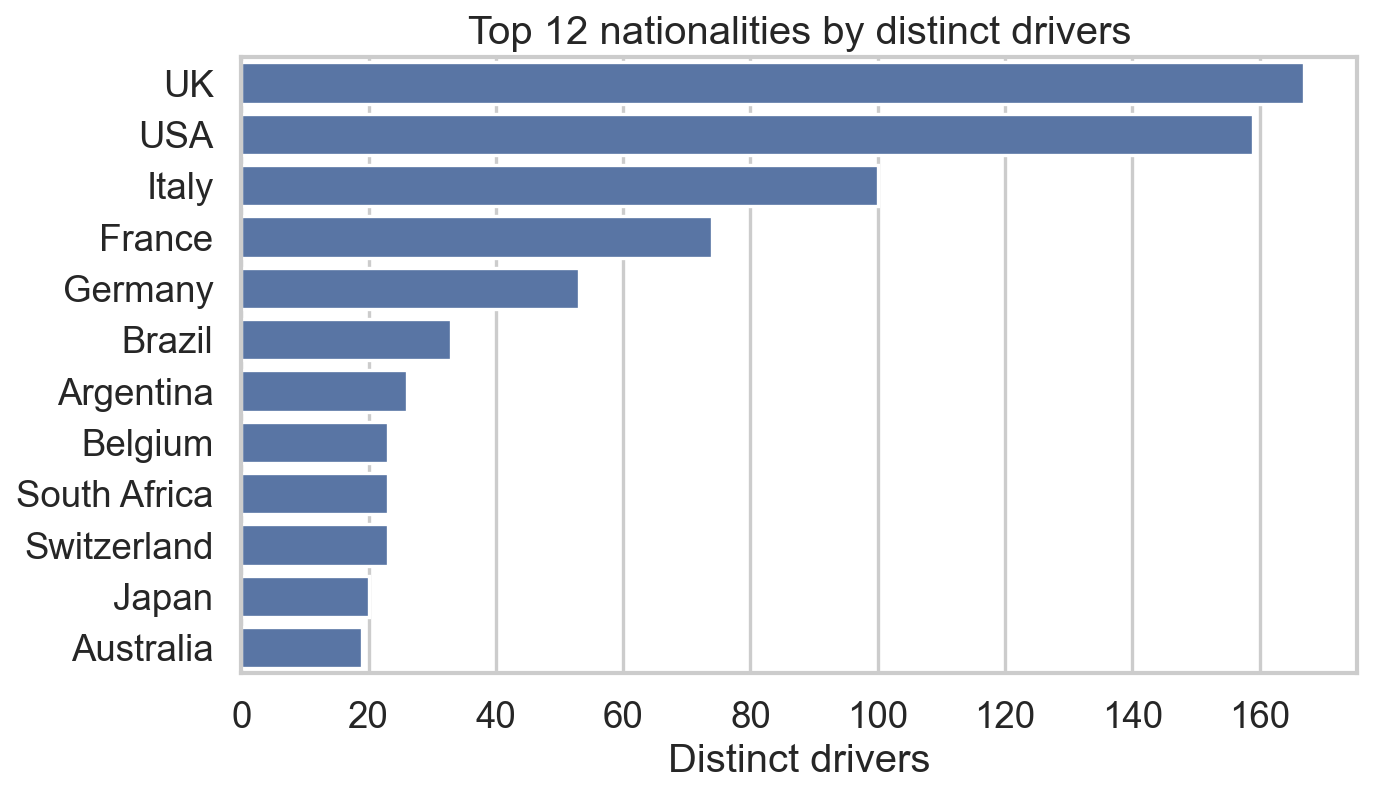
\includegraphics[width=0.78\textwidth]{04_top_nationalities.png}
  \caption{Top twelve nationalities by distinct drivers. British and
  Italian drivers dominate the home-race observations.}
  \label{fig:nat}
\end{figure}

\subsection{RQ1: paired t-test}
For every driver with at least one home and one away start, we form
the per-driver means $\bar\Delta_i^\text{home}$,
$\bar\Delta_i^\text{away}$ and the difference
$d_i = \bar\Delta_i^\text{home} - \bar\Delta_i^\text{away}$. The
pairing eliminates the between-driver confounder that an unpaired
test would absorb.

Across $n=440$ paired drivers, the mean difference is
$\bar d = +0.00265$ ($95\%$ CI $[-0.00534, +0.01064]$),
$t_{439}=0.65$, $p=0.515$, Cohen's $d=0.031$. We fail to reject
the null: at the aggregate level, F1 drivers do not perform
measurably better at home. Figure~\ref{fig:diff-hist} shows the
distribution of per-driver differences; Figure~\ref{fig:hvsa-pair}
shows the same comparison without pairing (boxplot and
mean-with-CI), which is visually identical and underscores the same
message.

\begin{figure}[H]
  \centering
  \begin{subfigure}{0.49\textwidth}
    \centering
    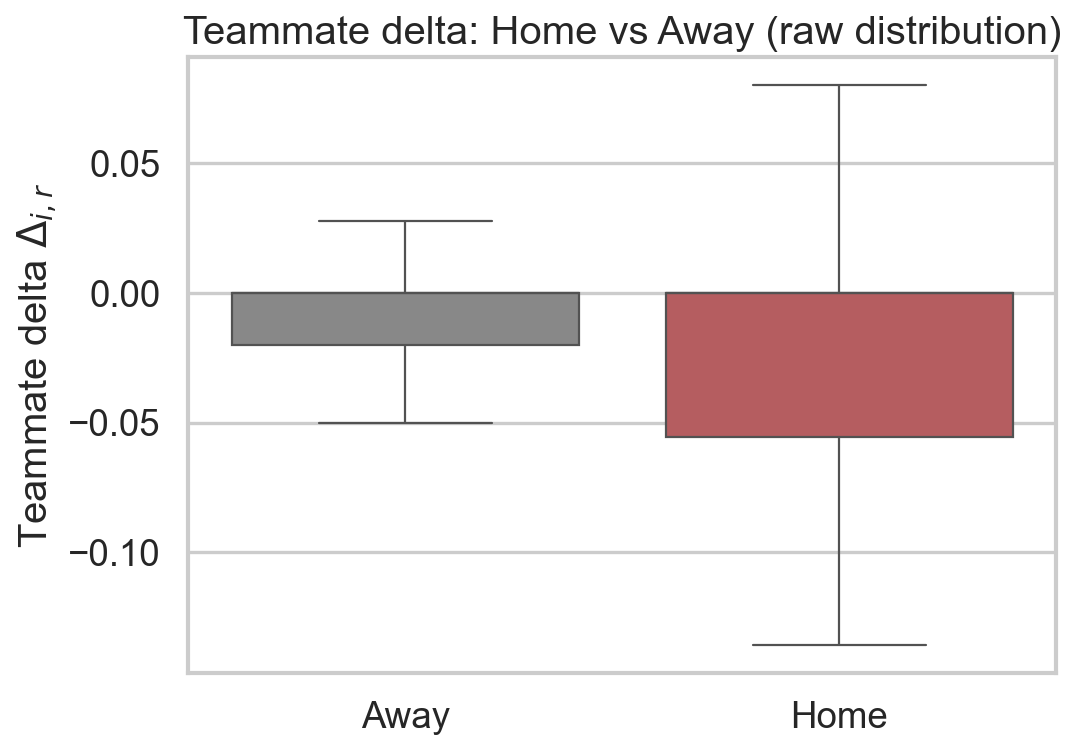
\includegraphics[width=\linewidth]{02_home_vs_away_box.png}
    \caption{Boxplots.}
  \end{subfigure}
  \hfill
  \begin{subfigure}{0.49\textwidth}
    \centering
    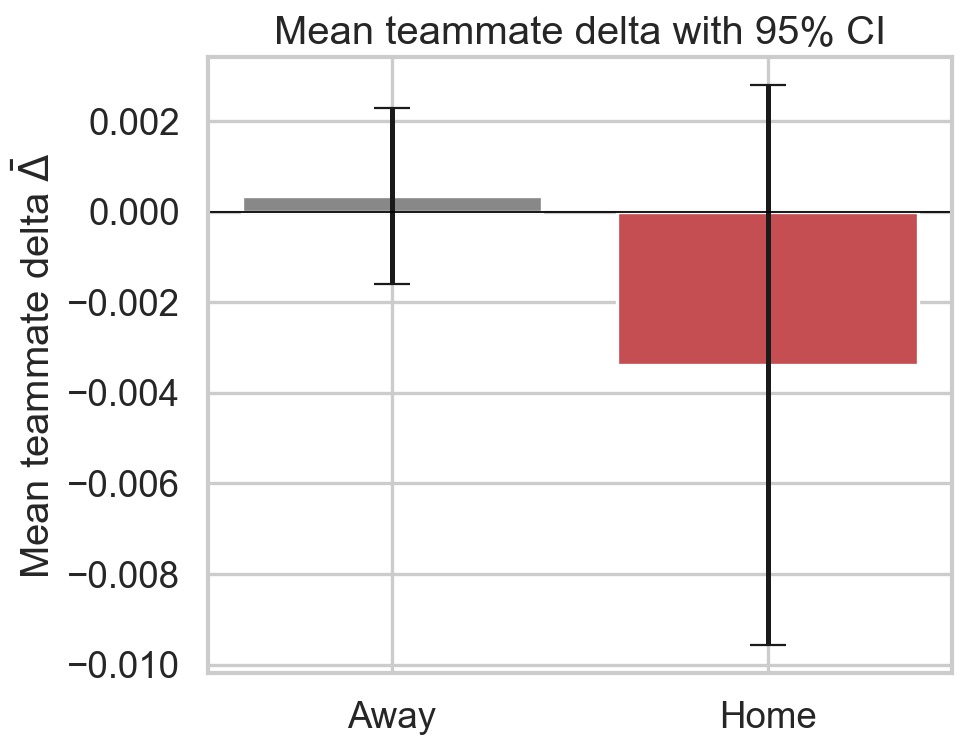
\includegraphics[width=\linewidth]{03_home_vs_away_meanci.png}
    \caption{Means with $95\%$ CIs.}
  \end{subfigure}
  \caption{Unpaired comparison of $\Delta_{i,r}$ between home and
  away starts.}
  \label{fig:hvsa-pair}
\end{figure}

\begin{figure}[H]
  \centering
  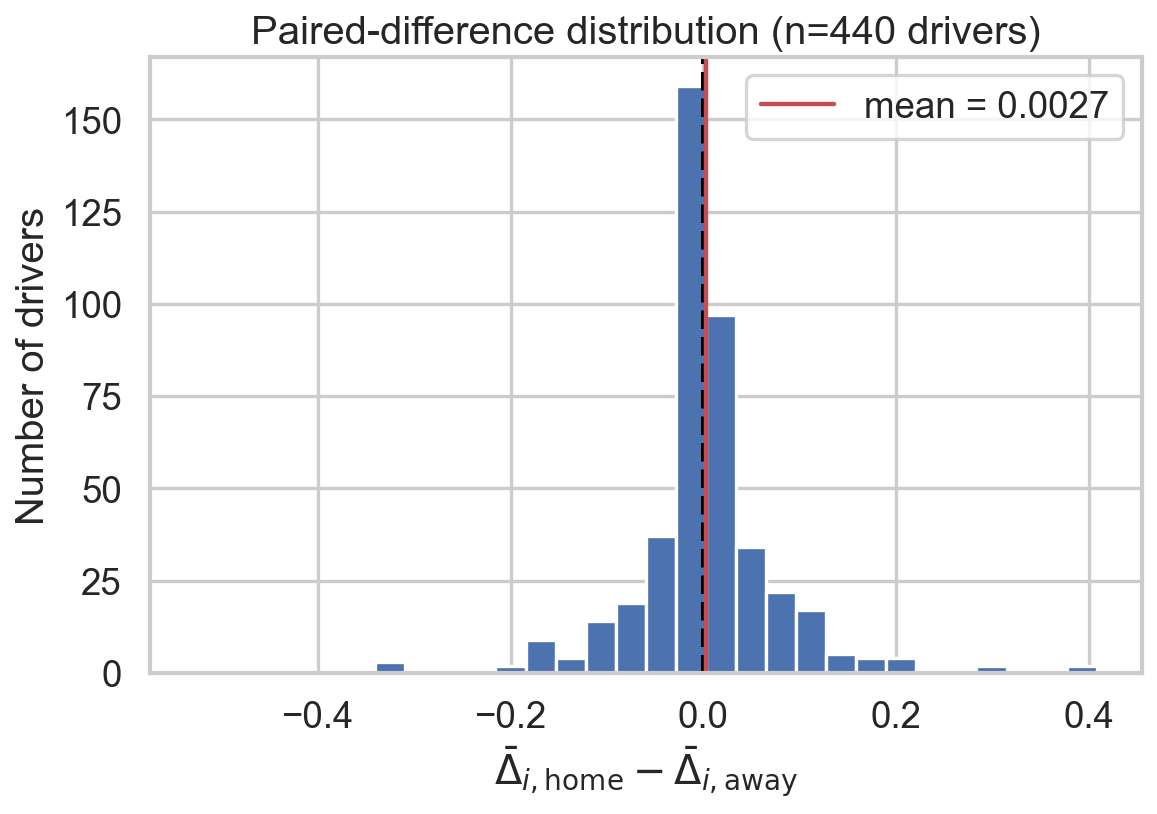
\includegraphics[width=0.72\textwidth]{07_paired_diff_hist.png}
  \caption{Per-driver paired differences $d_i$. The red line marks the
  mean ($+0.0027$); the distribution is symmetric around zero.}
  \label{fig:diff-hist}
\end{figure}

The corresponding per-driver effect picture
(Figure~\ref{fig:per-driver}) makes the same point at the individual
level: among the most-active drivers the home-minus-away difference
is positive about as often as it is negative, and the magnitudes do
not noticeably favour either sign.

\begin{figure}[H]
  \centering
  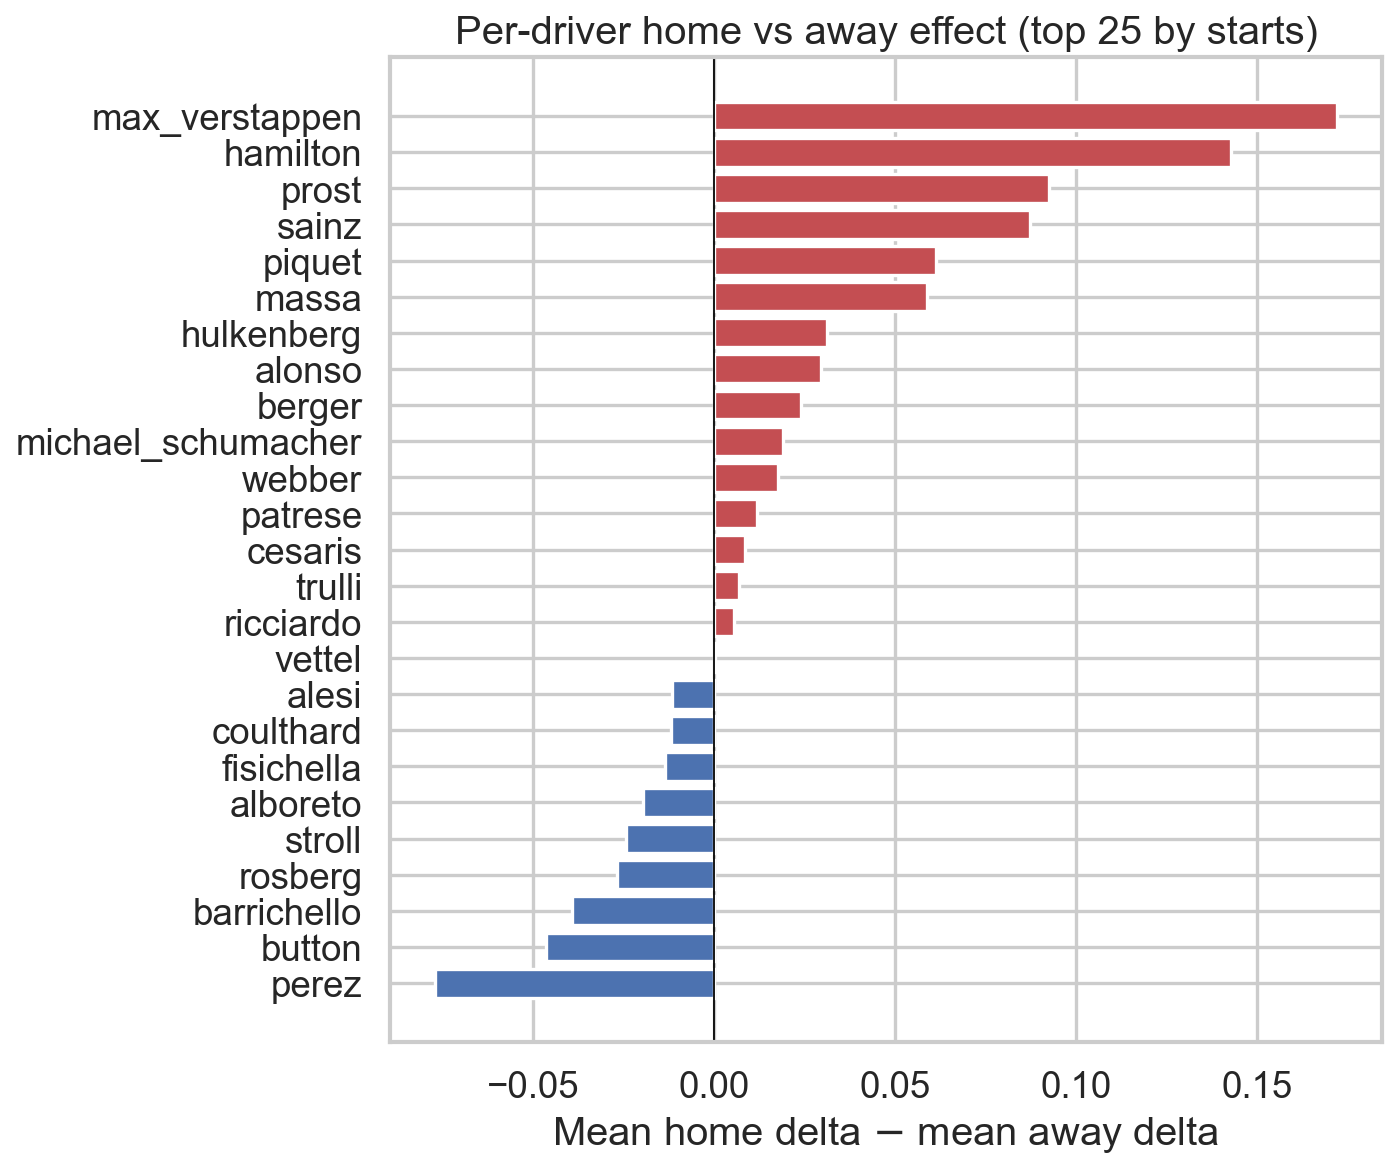
\includegraphics[width=0.85\textwidth]{06_per_driver_effect.png}
  \caption{Per-driver home$-$away mean $\Delta$ for the twenty-five
  drivers with the most starts. Red bars indicate the driver helped
  at home, blue bars indicate the opposite. The sign distribution is
  visibly symmetric.}
  \label{fig:per-driver}
\end{figure}

\subsection{RQ2: linear mixed-effects model}
The paired test collapses each driver to two numbers and assumes a
constant home effect. We relax both assumptions with a linear
mixed-effects model that allows a driver-specific random intercept
and an interaction between home and experience:
\begin{equation}
\Delta_{i,r} = \beta_0 + \beta_1 H_{i,r}+\beta_2 E_{i,r}
+\beta_3 (H_{i,r}\cdot E_{i,r}) + u_i + \varepsilon_{i,r},
\label{eq:lmm}
\end{equation}
with $u_i\sim\dnorm(0,\sigma_u^2)$ independent of
$\varepsilon_{i,r}\sim\dnorm(0,\sigma^2)$. Estimation is by REML in
\code{statsmodels.MixedLM}. Here $H$ is the home indicator and $E$ is
years since debut.

\begin{table}[H]
  \centering
  \caption{Mixed-effects estimates for Eq.~\eqref{eq:lmm}.}
  \label{tab:lmm}
  \begin{tabular}{lrrrr}
    \toprule
    Term & Estimate & SE & $z$ & $p$ \\
    \midrule
    Intercept            & $-0.00984$ & $0.00249$ & $-3.96$ & $7.6\!\times\!10^{-5}$ \\
    \code{home}          & $-0.00613$ & $0.00466$ & $-1.32$ & $0.188$ \\
    \code{experience}    & $-0.00143$ & $0.00029$ & $-4.96$ & $7.2\!\times\!10^{-7}$ \\
    \code{home$\times$experience} & $+0.00178$ & $0.00084$ & $+2.10$ & $0.035$ \\
    \midrule
    $\sigma_u^2$ (driver) & $0.00174$ & --- & --- & --- \\
    $\sigma^2$ (residual) & $0.02279$ & --- & --- & --- \\
    \bottomrule
  \end{tabular}
\end{table}

Three points stand out.
\begin{enumerate}
  \item The main effect of home is not significant ($p=0.188$),
  consistent with the paired test.
  \item The home$\times$experience interaction is positive and
  significant ($\hat\beta_3=+0.00178$, $p=0.035$). The total
  experience slope at home, $\hat\beta_2+\hat\beta_3\approx 0$, is
  essentially flat, whereas at away races experienced drivers slowly
  lose ground to younger teammates.
  \item The intraclass correlation is
  $\rho = \sigma_u^2/(\sigma_u^2+\sigma^2)\approx 0.071$: only $7\%$
  of residual variance is between-driver. The mixed structure is
  worth keeping but not load-bearing.
\end{enumerate}

Figure~\ref{fig:lmm-marg} visualises the interaction: rookies are
slightly worse at home than away, veterans are slightly better, and
the two lines cross around eight years of experience.

\begin{figure}[H]
  \centering
  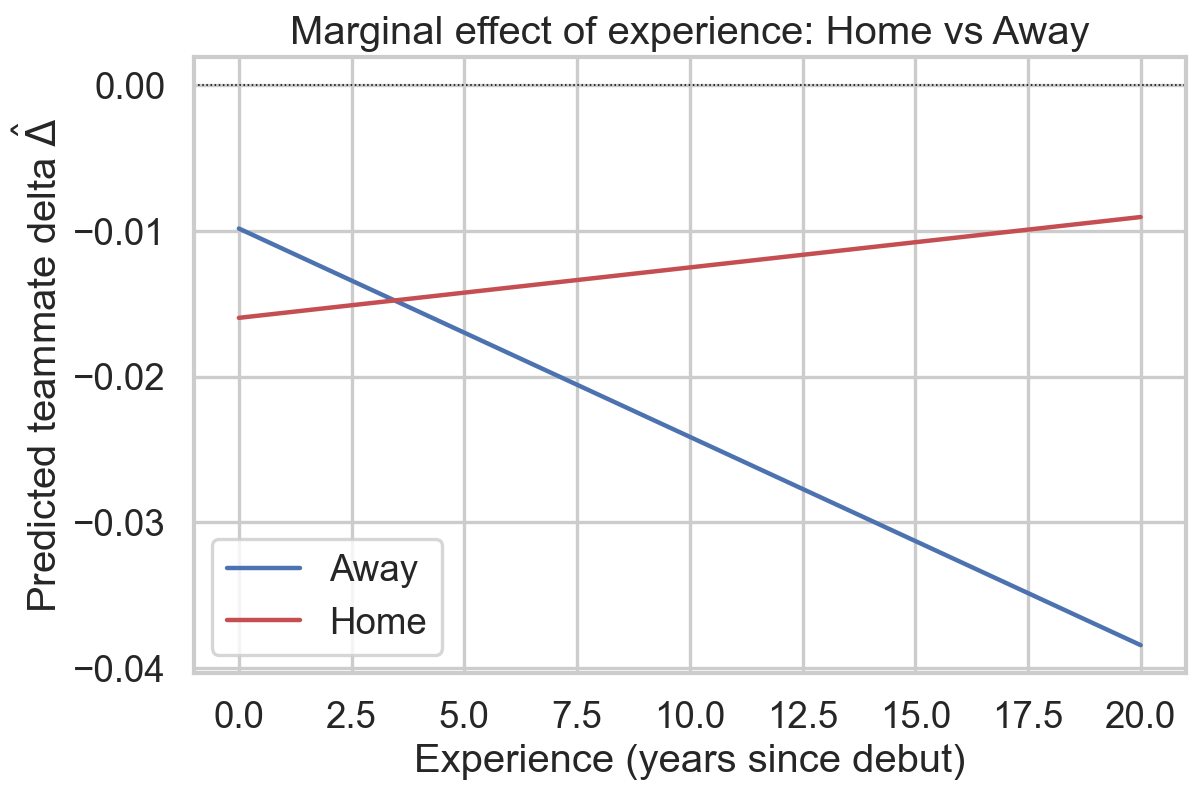
\includegraphics[width=0.72\textwidth]{08_mixedlm_marginal.png}
  \caption{Marginal mean of $\Delta_{i,r}$ from Eq.~\eqref{eq:lmm} as
  a function of experience, separately for home and away starts. The
  lines cross: the home crowd appears to neutralise the
  age-related drift seen at away races.}
  \label{fig:lmm-marg}
\end{figure}

\subsection{RQ3: XGBoost with time-series cross-validation}
A non-parametric predictor is fit on four features --- experience,
home indicator, grid position, and circuit-baseline crash rate ---
using XGBoost ($100$ trees, depth $4$, learning rate $0.1$). Random
$k$-fold cross-validation would leak information from later seasons
into earlier folds. We instead use a five-fold expanding-window
backtest in which training data always precede test data in time.

\begin{table}[H]
  \centering
  \caption{Expanding-window XGBoost backtest. Errors are on the
  $[0,1]$ normalised scale.}
  \label{tab:backtest}
  \begin{tabular}{rllrr}
    \toprule
    Fold & Train years & Test years & RMSE & MAE \\
    \midrule
    1 & 1950--1971 & 1971--1982 & $0.162$ & $0.106$ \\
    2 & 1950--1982 & 1982--1992 & $0.137$ & $0.081$ \\
    3 & 1950--1992 & 1992--2004 & $0.145$ & $0.086$ \\
    4 & 1950--2004 & 2004--2015 & $0.152$ & $0.099$ \\
    5 & 1950--2015 & 2015--2026 & $0.140$ & $0.093$ \\
    \midrule
    \textbf{Mean} & & & $\mathbf{0.147}$ & $\mathbf{0.093}$ \\
    \textbf{SD}   & & & $0.009$  & $0.009$  \\
    \bottomrule
  \end{tabular}
\end{table}

The error is stable across seventy years of regulation drift
(Figure~\ref{fig:backtest}); an MAE of $0.093$ on the $[0,1]$ scale
corresponds to roughly two modern points per race. Figure~\ref{fig:xgb-imp}
ranks the four features by gain importance: grid position dominates,
followed by experience and the circuit-baseline crash rate; the
\code{home\_race} flag carries little raw importance, which mirrors
the LMM finding that the main home effect is small. The SHAP
dependence plot (Figure~\ref{fig:shap-exp}) reproduces the LMM
interaction visually: at every experience level the home dots sit
slightly higher than the away dots, with the gap widening for veterans.

\begin{figure}[H]
  \centering
  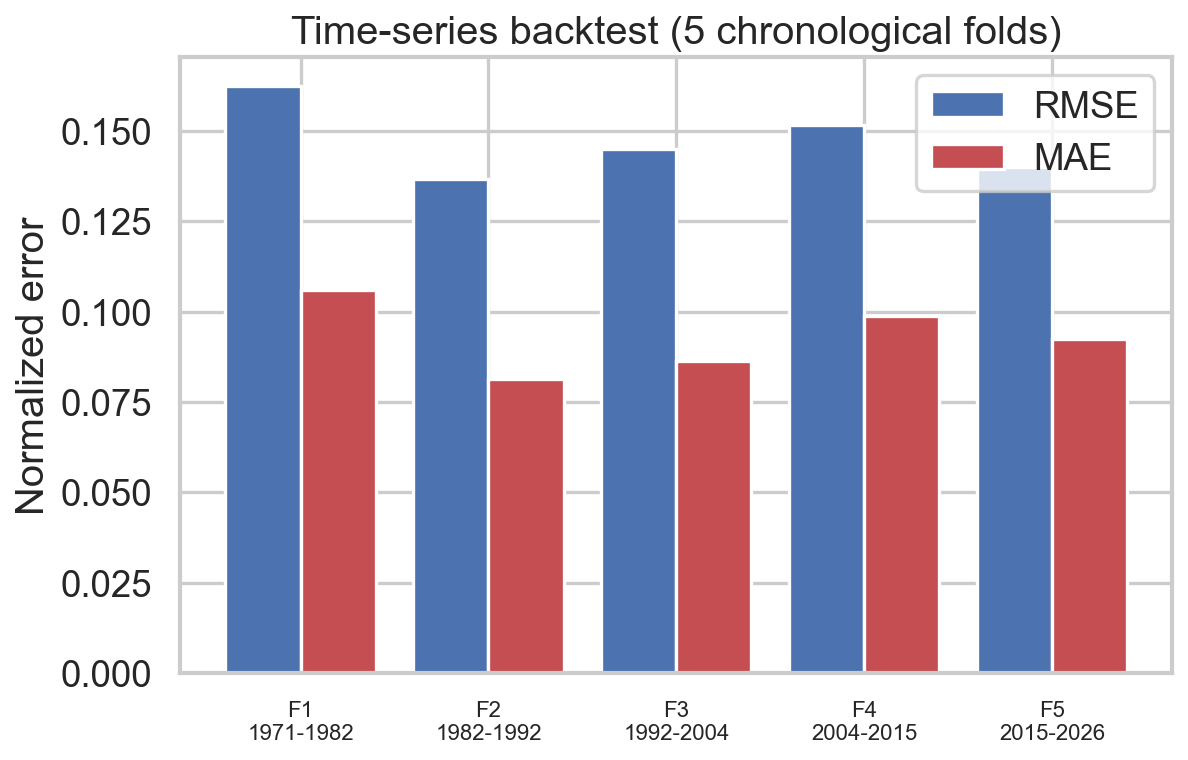
\includegraphics[width=0.78\textwidth]{13_backtest_folds.png}
  \caption{Expanding-window backtest: RMSE and MAE per chronological
  fold. The model generalises stably across regulation eras.}
  \label{fig:backtest}
\end{figure}

\begin{figure}[H]
  \centering
  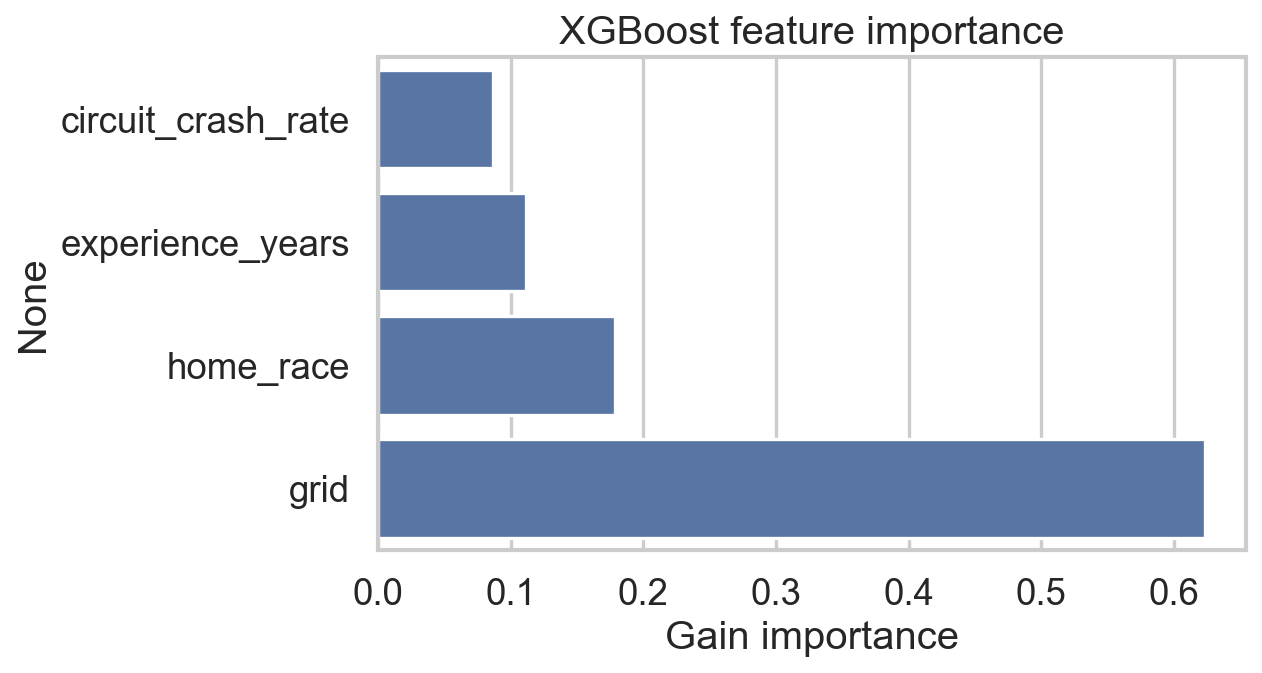
\includegraphics[width=0.7\textwidth]{09_xgb_importance.png}
  \caption{XGBoost gain importance of the four predictors. Grid
  dominates, \code{home\_race} contributes little on its own.}
  \label{fig:xgb-imp}
\end{figure}

\begin{figure}[H]
  \centering
  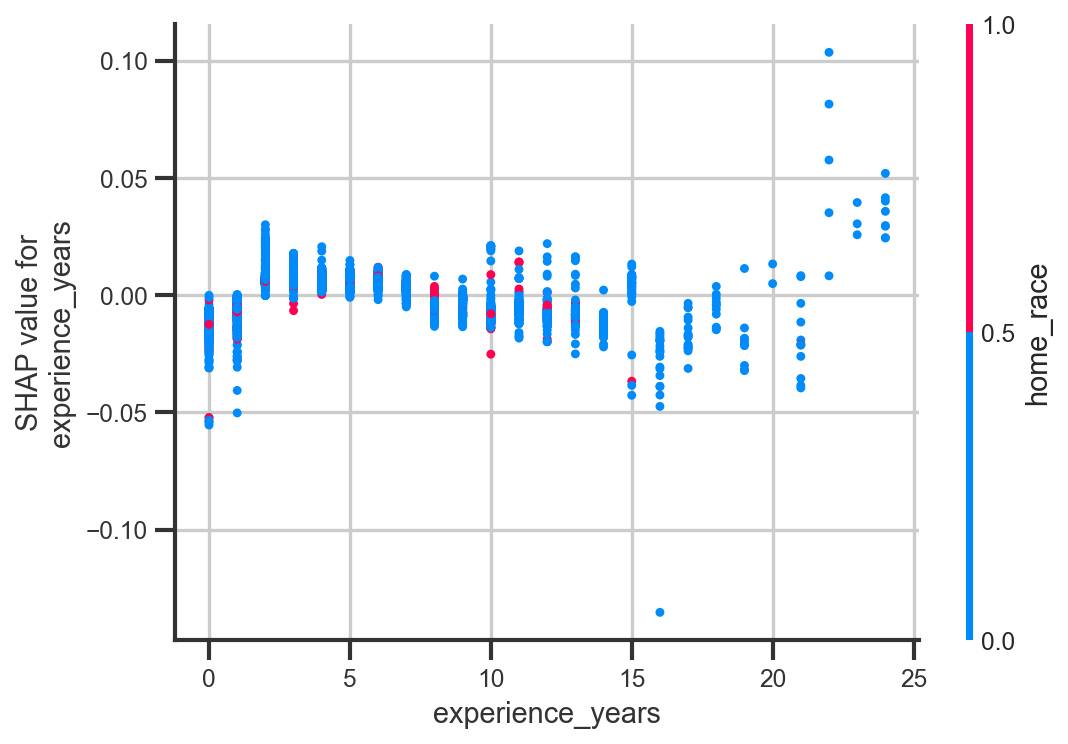
\includegraphics[width=0.72\textwidth]{11_shap_dependence_exp_home.png}
  \caption{SHAP dependence: contribution of \code{experience\_years}
  to the XGBoost prediction, coloured by \code{home\_race}. The
  vertical separation between home (red) and away (blue) grows with
  experience --- visual confirmation of $\hat\beta_3>0$.}
  \label{fig:shap-exp}
\end{figure}

\begin{figure}[H]
  \centering
  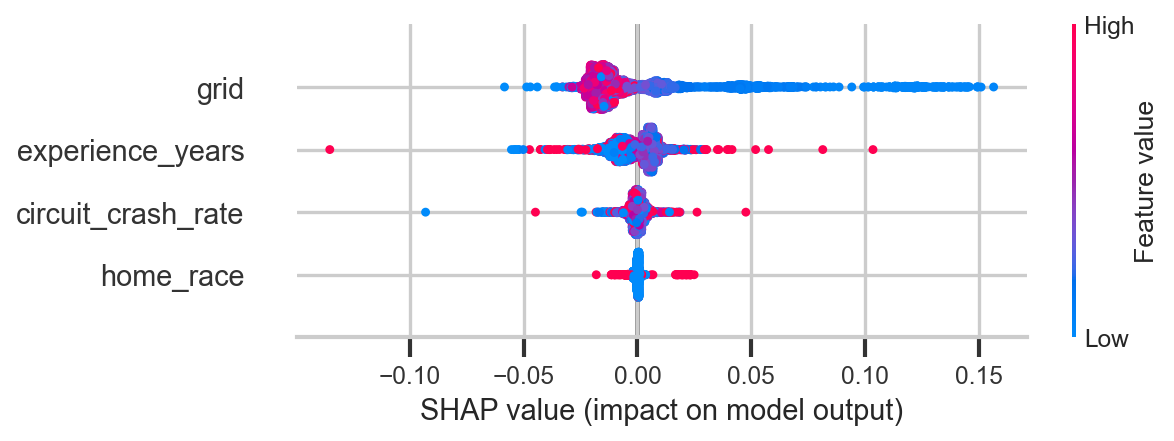
\includegraphics[width=0.75\textwidth]{10_shap_beeswarm.png}
  \caption{SHAP beeswarm summarising the contribution of each feature
  to each individual prediction. Grid is the dominant signal and
  behaves monotonically; \code{home\_race} is concentrated near zero
  with a small but visible spread.}
  \label{fig:shap-bee}
\end{figure}

\subsection{Limitations}
A statistically careful reader will object to several aspects of
this design.
\begin{enumerate}
  \item \textbf{Class imbalance.} Only $9.3\%$ of starts are home
  starts; statistical power on $\hat\beta_1$ is therefore modest.
  \item \textbf{Causal language.} Observational data cannot fully
  resolve confounders such as constructor selection effects (a team
  may field a stronger car at a home race for sponsorship reasons).
  \item \textbf{Heterogeneous nationalities.} Edge cases
  (\textit{Argentine-Italian}, \textit{Rhodesian}, \textit{East German})
  require mapping decisions whose sensitivity we do not exhaustively
  audit here.
  \item \textbf{Static features.} The covariate set is deliberately
  small. A richer study would add weather, tyre selection, in-season
  form, and constructor-by-circuit historical strength.
\end{enumerate}

\subsection{Take-home}
The conventional wisdom of a measurable home-crowd boost is
\emph{not} supported in F1. The aggregate effect is statistically
indistinguishable from zero. A small, secondary interaction with
experience does emerge: young drivers underperform slightly at home,
veterans overperform slightly, and the two cancel in the mean. The
methodological lesson is that the construction of an
\emph{era-adjusted, teammate-relative} target is what allows three
otherwise incomparable techniques --- a paired test, a hierarchical
model, and a boosted-tree predictor --- to converge on the same
substantive answer.

% =====================================================================
\section{Pit-Stop Strategy}\label{sec:pit}
% =====================================================================

\subsection{Question and motivation}
Pit strategy decides as many races as raw pace. A model that can
assign a real-time probability to an imminent pit stop supports
undercut detection, compound-choice analysis, and post-race review.
We pursue four research questions:
\begin{enumerate}
  \item Can a sequence model trained on historical telemetry predict
  pit-stop events with operationally useful precision and recall?
  \item Which stochastic process best describes the pit hazard as a
  function of tyre age?
  \item Is there a statistical relationship between pit-crew speed
  and constructor championship performance?
  \item Can a driver's reaction time under a Virtual Safety Car (VSC)
  predict whether they finish ahead of their qualifying position?
\end{enumerate}

\subsection{Data and feature engineering}
Per-lap telemetry is sourced from the FastF1 API: lap speed
(mean, max, std), RPM, throttle, brake, DRS, gear, sector times,
tyre compound, and tyre age. Historical pit durations come from the
Ergast database. The BiLSTM was trained on the full $2018$--$2025$
record ($152{,}475$ valid laps, $4{,}818$ pit stops, $3.16\%$
positive rate). The descriptive figures in this section are
regenerated from the $2024$ subset (23 races, $24{,}138$ valid laps,
$731$ pit stops, $3.03\%$ rate); a full $2018$--$2025$
regeneration is reproducible by running
\code{src/pit\_stop\_strategy/download\_subset.py} with
\code{--years 2018 2019 2020 2021 2022 2023 2024 2025}.

Features are organised in six groups: race state (lap, position,
track status); tyre degradation (tyre life, performance decay,
relative age); pace evolution (lap-time delta, rolling pace mean,
degradation slope); telemetry; traffic and DRS proximity; and
strategy priors (historical pit lap, pit-window delta).

\paragraph{Leakage prevention.}
Raw timing columns that would directly reveal a pit stop
(\code{PitInTime}, \code{PitOutTime}, \code{LapTime},
\code{Sector1-3Time}, \code{SessionTime}) are dropped before
modelling. The \code{historical\_pit\_lap} feature is computed only
on the training split and joined onto the test set.

\paragraph{Sequence construction.}
Within each \code{(Year, RaceID, DriverNumber)} group, a length-$20$
sliding window advances one lap at a time. The window's label is the
\code{HasPitStop} indicator on its final lap. Groups shorter than
twenty laps are discarded. The choice of window length is a
compromise: shorter windows lose long-horizon tyre information; longer
windows fragment the stint, since a typical stint is $15$--$25$ laps.
Length-$20$ aligns with the empirical mean pit lap of $27.7$ minus the
empirical mean tyre life of $15.1$, plus enough slack to see the
build-up to a stop.

\begin{figure}[H]
  \centering
  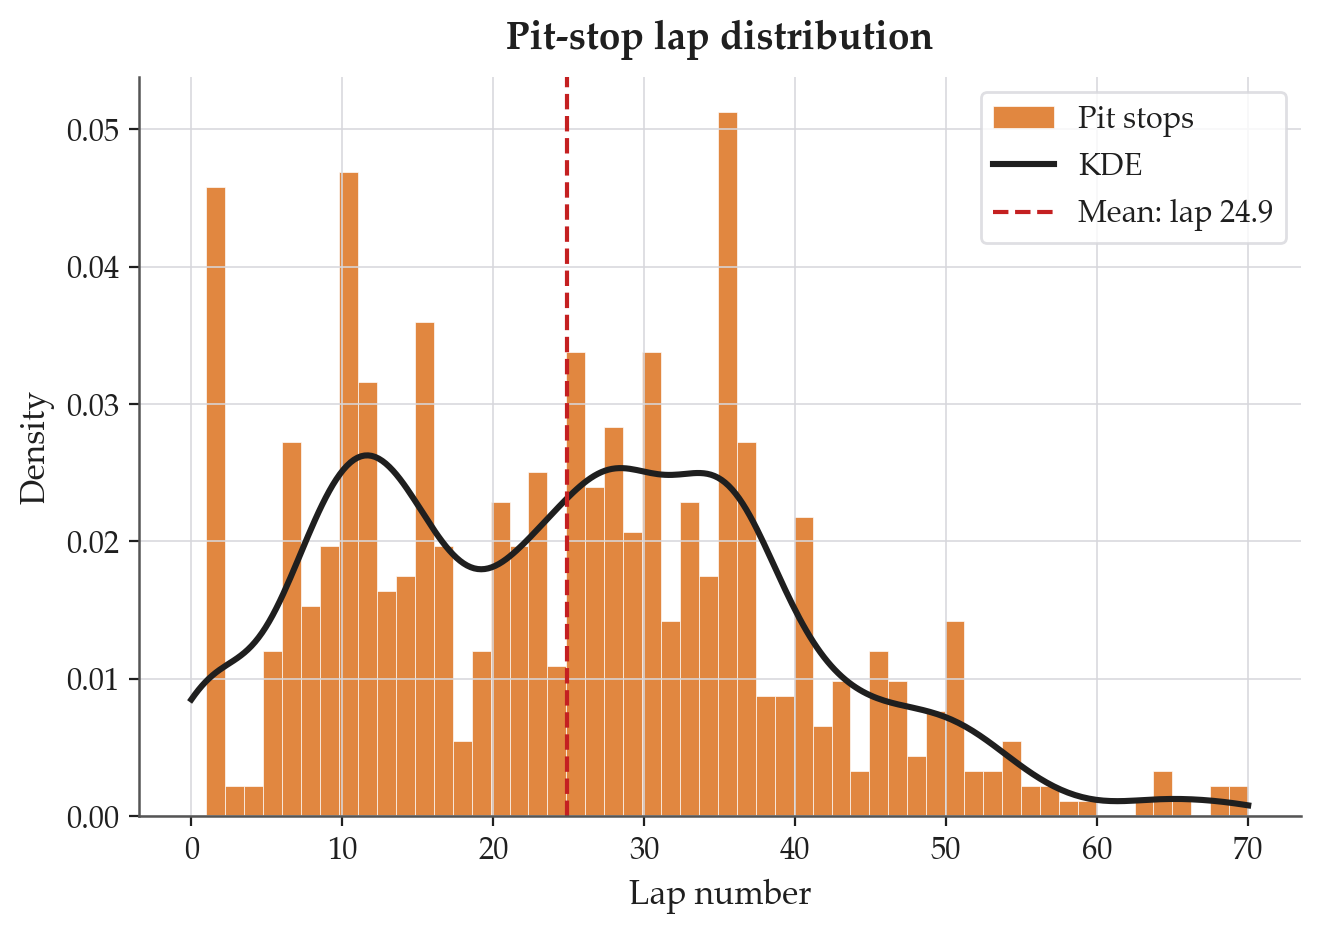
\includegraphics[width=0.85\textwidth]{01c_pitstop_lap_dist.png}
  \caption{Empirical distribution of the pit-stop lap across the
  $2024$ season. The mean pit lap is $24.9$; the primary pit window
  concentrates around laps $20$--$30$.}
  \label{fig:pit-laps}
\end{figure}

\begin{figure}[H]
  \centering
  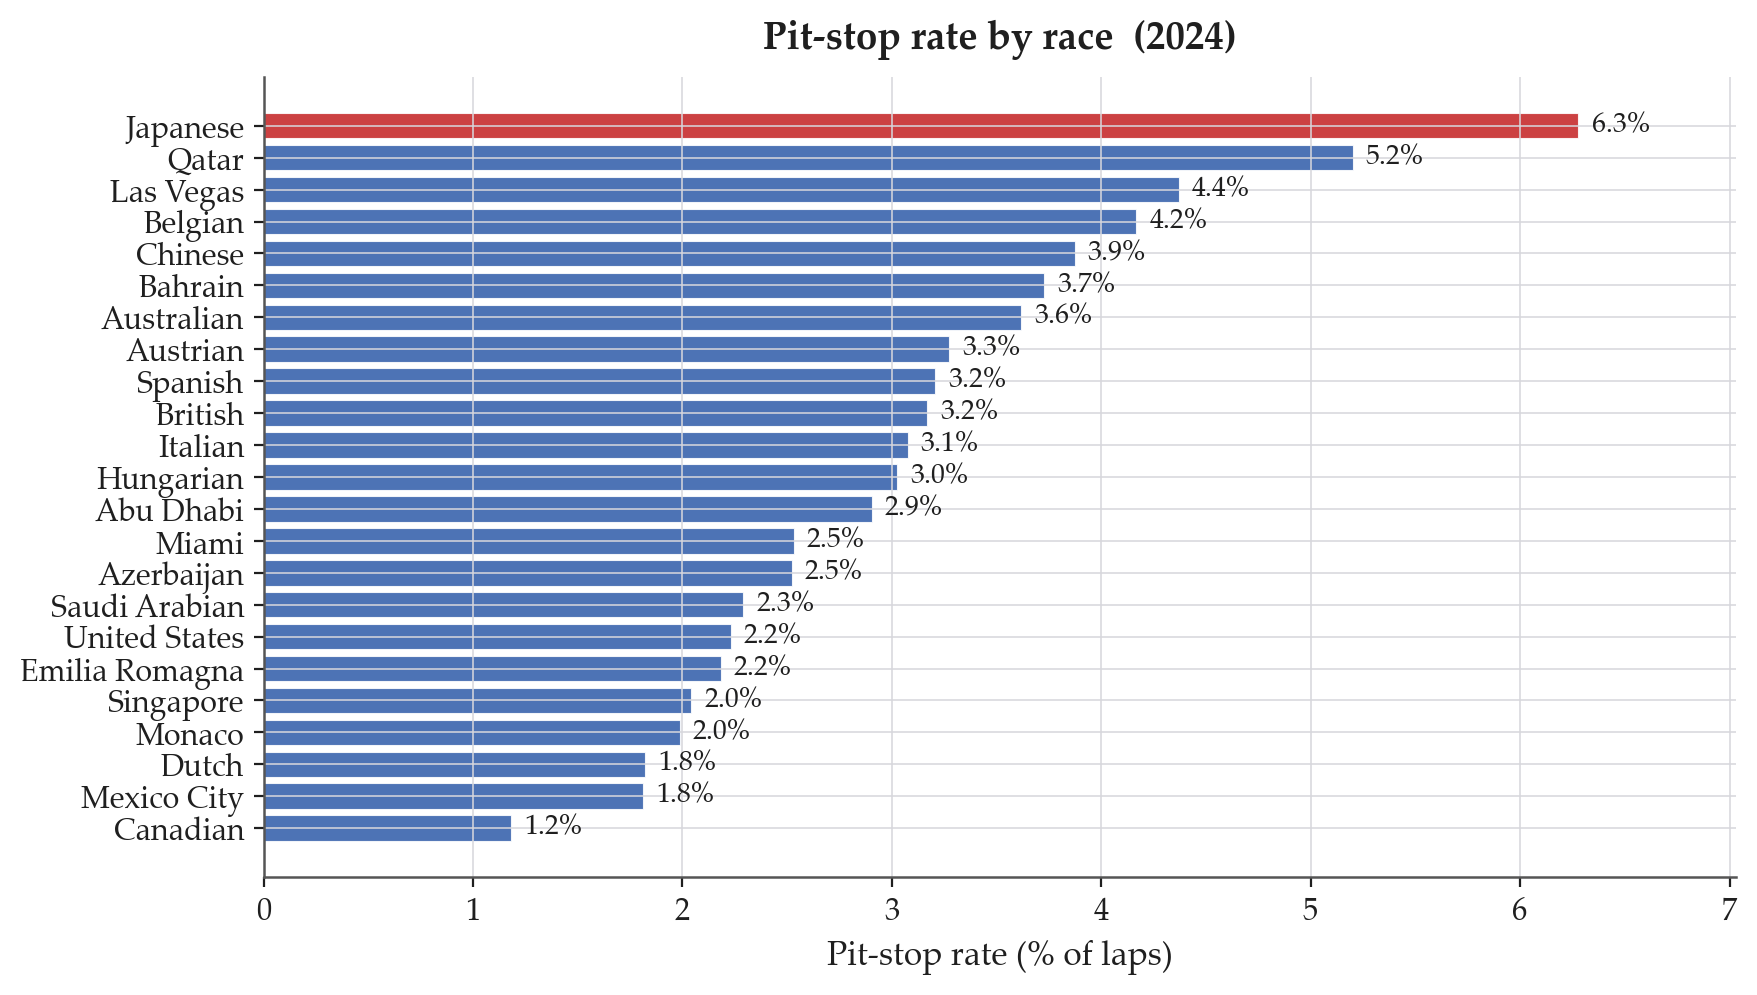
\includegraphics[width=0.85\textwidth]{01d_pit_rate_season.png}
  \caption{Pit-stop rate per race across the $2024$ season (one bar
  per round, sorted by rate). The Japanese Grand Prix at Suzuka
  produced the highest rate ($6.3\%$); the Canadian GP the lowest
  ($1.2\%$). When multi-season data is available
  \code{visualize.py} automatically switches to a per-season view.}
  \label{fig:pit-rate-season}
\end{figure}

\subsection{Bidirectional LSTM pit-stop predictor}
The architecture is a three-layer BiLSTM with progressive hidden
sizes followed by two dense layers; full dimensions are listed in
Table~\ref{tab:bilstm-arch}. Each recurrent block is followed by
dropout and batch normalisation along the feature dimension.

\begin{table}[H]
  \centering
  \caption{Pit-stop BiLSTM architecture. ``Output dim'' includes the
  $\times 2$ from the bidirectional pass.}
  \label{tab:bilstm-arch}
  \small
  \begin{tabular}{llrrr}
    \toprule
    Layer & Type & Hidden & Output dim & Dropout \\
    \midrule
    1 & BiLSTM   & $256$ & $512$ & $0.20$ \\
    2 & BiLSTM   & $128$ & $256$ & $0.30$ \\
    3 & BiLSTM   & $\phantom{0}64$ & $128$ & $0.30$ \\
    4 & Dense (ReLU) & $\phantom{0}64$ & $\phantom{0}64$ & $0.20$ \\
    5 & Dense (ReLU) & $\phantom{0}32$ & $\phantom{0}32$ & --- \\
    6 & Output (sigmoid) & --- & $\phantom{00}1$ & --- \\
    \bottomrule
  \end{tabular}
\end{table}

The optimiser is Adam at learning rate $10^{-4}$ with a
\code{ReduceLROnPlateau} schedule, batch size $64$, gradient
clipping at norm $1$, early stopping with patience eight on
validation AUC-PR. Class imbalance is handled by a positive-class
weight in \code{BCEWithLogitsLoss}; the decision threshold is chosen
to maximise the F1 score on the precision-recall curve rather than
defaulting to $0.5$.

The train/test split is strictly temporal: all seasons before $2025$
form the training set and $2025$ is held out, mirroring the
operational scenario of a model trained on history that must
generalise to a new season.

\paragraph{Results.}
On true-pit laps in the held-out $2025$ season the trained BiLSTM
assigns a mean probability of $83.8\%$, against a near-zero baseline
on non-pit laps. The held-out ROC AUC is $\approx 0.99$ and the
held-out average precision $\approx 0.83$ --- a strong discriminative
signal despite the $3.16\%$ positive rate. The trained model weights
are shipped under \code{outputs/pit\_stop\_strategy/models/} so the
inference figures can be reproduced once the FastF1 telemetry CSVs
are present locally.

\subsection{Survival and stochastic modelling}
\subsubsection{Pace decay and PACF}
Raw lap times are non-stationary: fuel burn pulls them down, tyre
wear pushes them up, traffic and weather perturb them. We compute the
partial autocorrelation function (PACF) within each stint to identify
the dominant lag and then apply a first-difference AR(1) filter
$\Delta X_t = X_t - X_{t-1}$, producing a stationary
\code{Stationary\_PaceDecay} series that isolates tyre-induced
degradation from lap-to-lap noise.

\subsubsection{Cox proportional hazards}
Treating tyre age as the duration and \code{HasPitStop} as the event,
we fit a Cox proportional-hazards model with
\code{Stationary\_PaceDecay} and \code{traffic\_pressure} as
covariates (\code{lifelines}). The partial hazard, min--max
normalised, supplies a per-lap pit probability baseline alongside
the BiLSTM output.

\subsubsection{Team risk profiles via mean and variance of stopping tyre life}
For every pit-stop event we record \code{TyreLife} at the moment of
stopping. Aggregating by constructor over the $2024$ subset gives
Table~\ref{tab:team-risk}: low-variance teams (Red Bull, Ferrari)
operate within a tight strategic window; high-variance teams (Kick
Sauber, Williams) react opportunistically to Safety Cars and
competitor undercuts.

\begin{table}[H]
  \centering
  \caption{Stopping tyre life by team, $2024$ season.}
  \label{tab:team-risk}
  \begin{tabular}{lcc}
    \toprule
    Team & Mean tyre life $\E[X]$ & Variance $\Var(X)$ \\
    \midrule
    Red Bull Racing & $19.5$ & $\phantom{0}83.4$ \\
    Ferrari         & $18.3$ & $\phantom{0}84.5$ \\
    McLaren         & $20.2$ & $\phantom{0}94.4$ \\
    Aston Martin    & $17.5$ & $\phantom{0}95.0$ \\
    Mercedes        & $19.3$ & $102.1$ \\
    RB              & $16.7$ & $117.3$ \\
    Alpine          & $18.1$ & $128.5$ \\
    Williams        & $17.3$ & $140.4$ \\
    Kick Sauber     & $18.5$ & $160.7$ \\
    \bottomrule
  \end{tabular}
\end{table}

\begin{figure}[H]
  \centering
  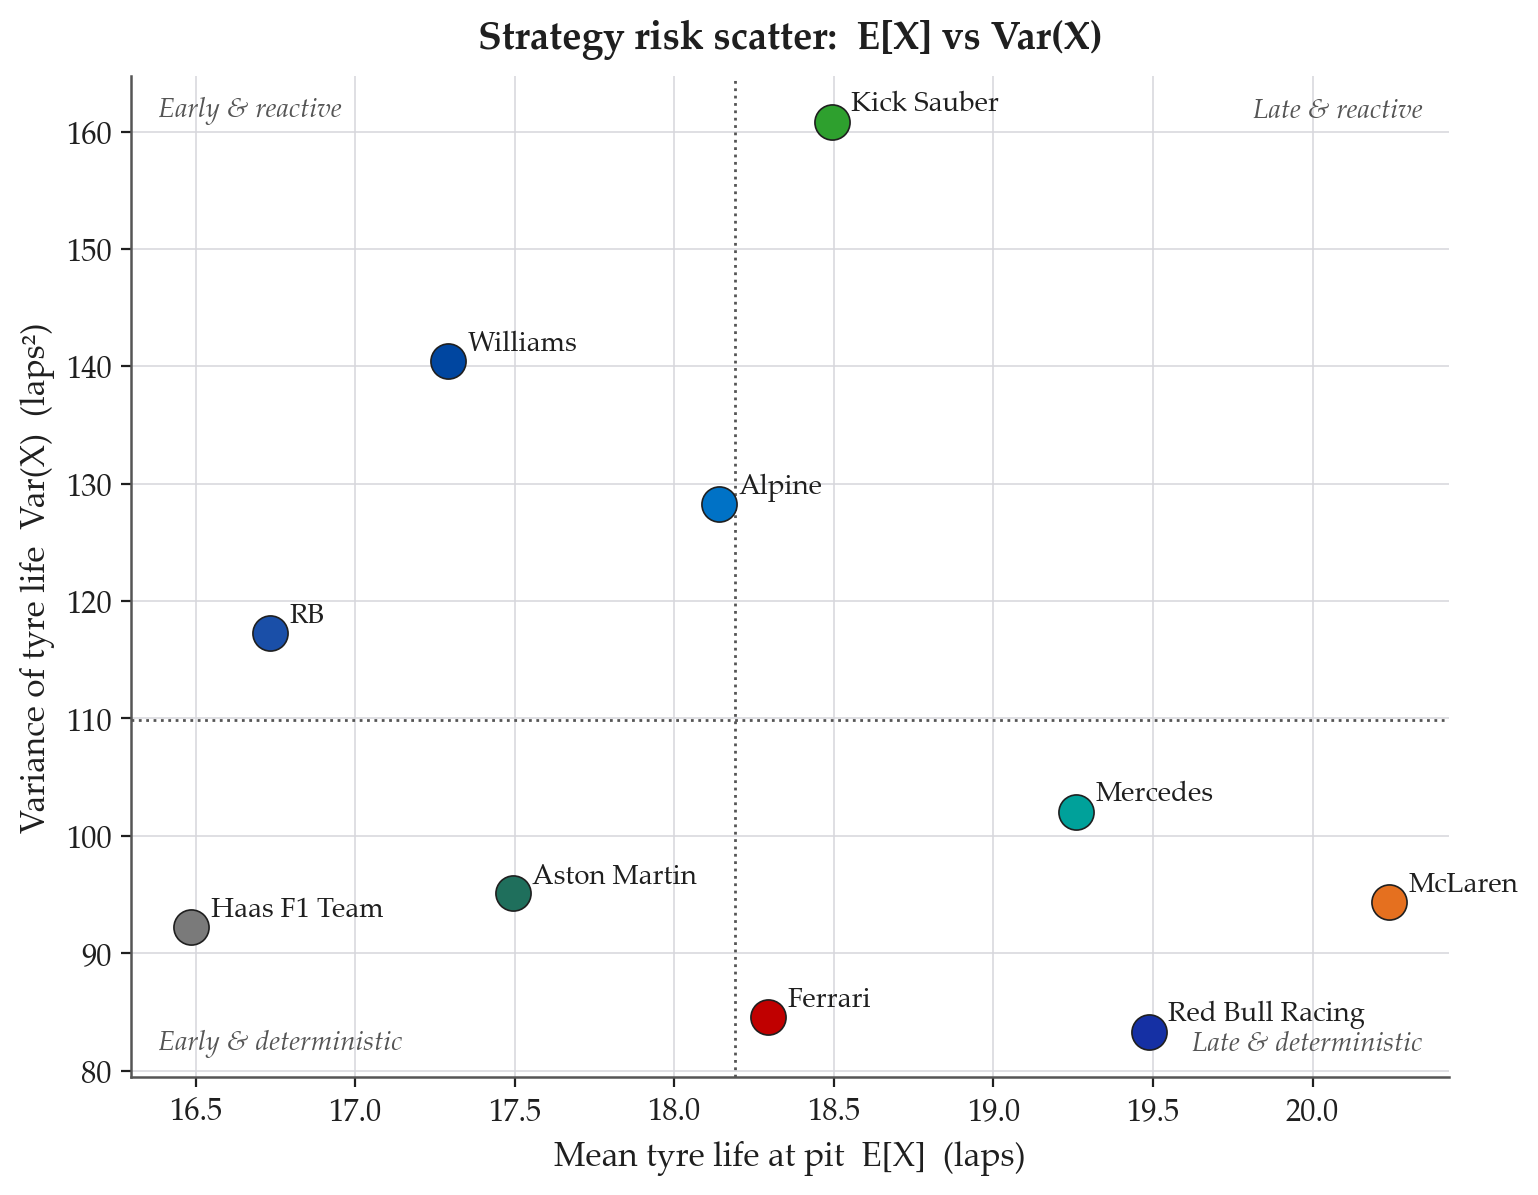
\includegraphics[width=0.82\textwidth]{04a_risk_scatter.png}
  \caption{Mean vs.\ variance of stopping tyre life by constructor,
  $2024$ season. Bottom-right (Ferrari, Red Bull, Mercedes) =
  late-deterministic strategy; top-left (Kick Sauber, Williams) =
  reactive/opportunistic.}
  \label{fig:pit-team-scatter}
\end{figure}

\begin{figure}[H]
  \centering
  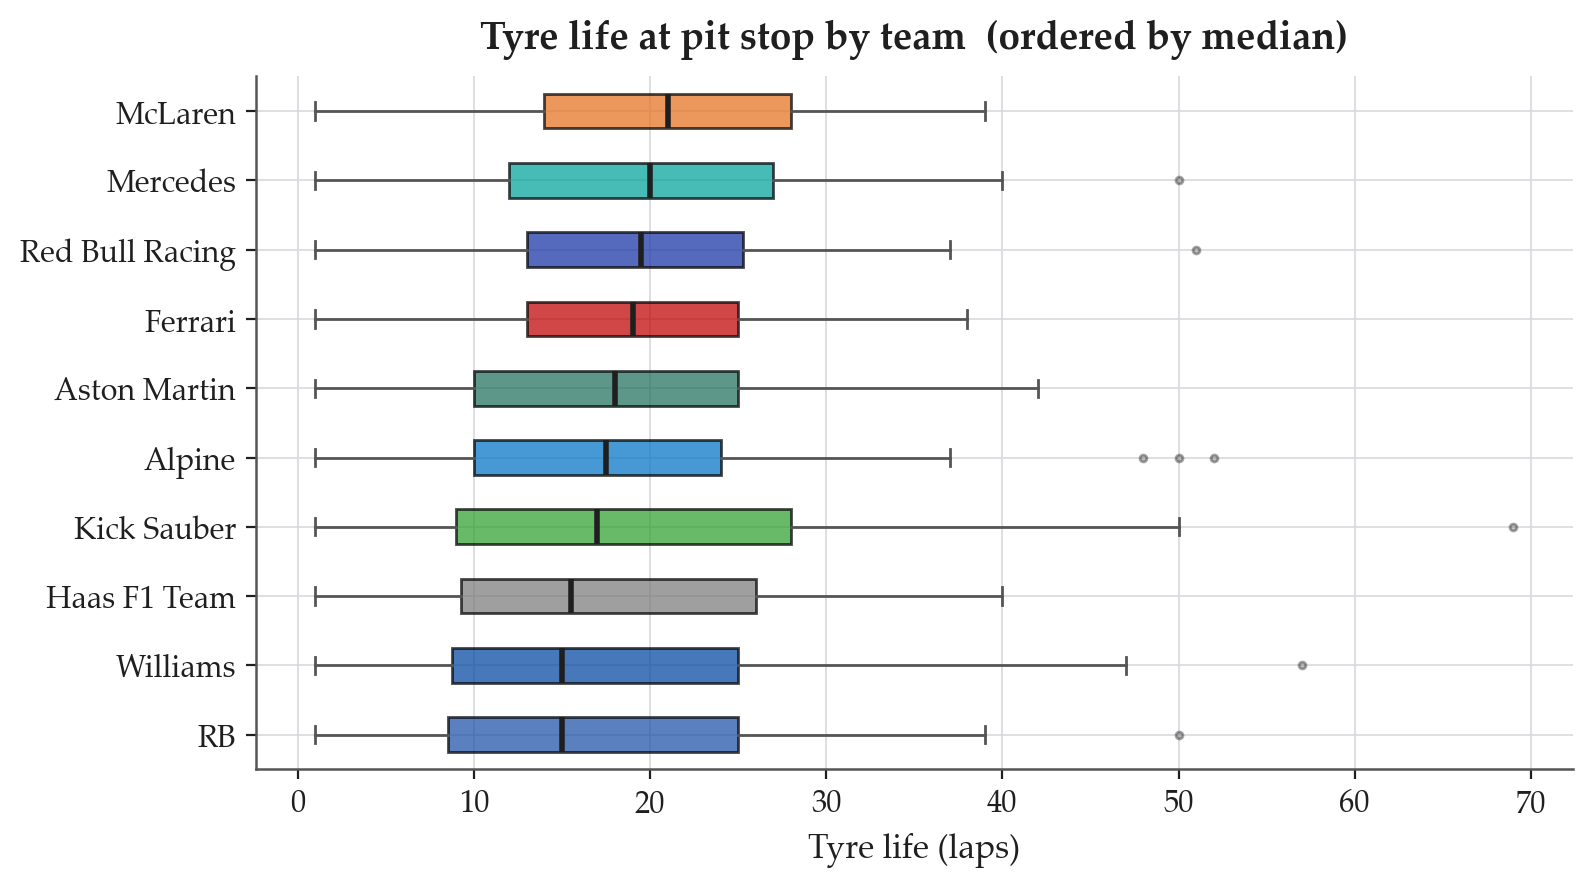
\includegraphics[width=0.82\textwidth]{04b_team_tyrelife_box.png}
  \caption{Distribution of stopping tyre life by team, ordered by
  median ($2024$ season). The IQR width directly visualises each
  team's strategic flexibility.}
  \label{fig:pit-team-box}
\end{figure}

\begin{figure}[H]
  \centering
  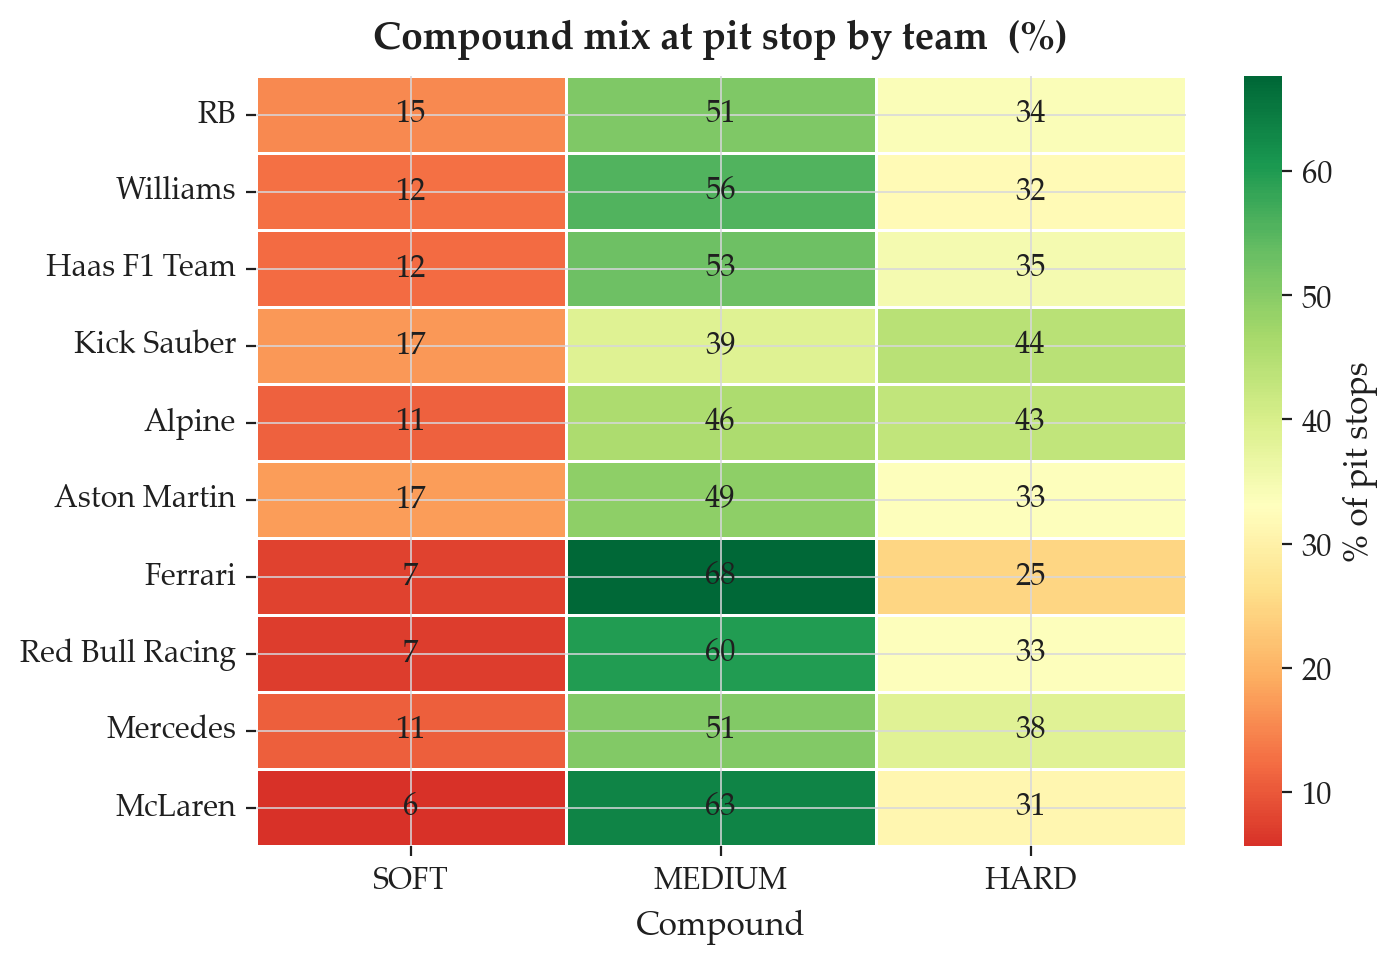
\includegraphics[width=0.82\textwidth]{04c_compound_mix_heatmap.png}
  \caption{Compound mix at pit stop by team, $2024$ season
  (row-normalised percentages). Green cells indicate compound choices
  that dominate a team's strategy; red cells indicate compounds
  they rarely select.}
  \label{fig:pit-team-compound}
\end{figure}

\subsubsection{Welch's t-test for \code{traffic\_pressure}}
To confirm that the engineered traffic-pressure feature carries
predictive value beyond the raw telemetry it is built from, we
compare \code{Stationary\_PaceDecay} between high and low traffic
conditions via Welch's unequal-variance $t$-test. The two
distributions differ significantly at the conventional level,
justifying the feature's inclusion.

\subsection{Strategic regression and VSC agility}
\subsubsection{Pit-crew speed and championship points}
The Ergast pit-stop log gives the median pit-stop duration per
constructor. A Pearson correlation against cumulative championship
points (constructors with $>100$ career points only, to exclude
historical one-race entries) provides a direct quantitative link
between operational pit-crew speed and championship performance.

\subsubsection{VSC tactical agility score}
For each driver--race we detect VSC/SC deployments from the
\code{Stochastic\_Shock\_VSC\_SC} flag and measure the number of
laps between deployment and pit. The mean is the driver's
\code{Agility\_Score}; drivers who do not pit during a VSC receive
a penalty of $5.0$ laps, representing a missed opportunity.

\subsubsection{Random-forest outcome classifier}
A $100$-tree random forest predicts whether a driver finishes ahead
of their qualifying position using four features:
\code{GridPos}, \code{Agility\_Score},
\code{PaceDecay} (the AR(1)-filtered degradation slope) and
\code{Mean\_Pit\_Prob} (the BiLSTM probability averaged over the
race). When \code{Agility\_Score} feature importance exceeds $0.15$
the framework reports tactical VSC reaction as a highly significant
driver of upward grid mobility.

\subsection{Overtake classification}
\code{overtake\_analysis.py} builds lap-by-lap position matrices per
race and detects every pair-wise position swap among the top ten.
A swap is labelled \emph{strategic} if either driver pitted within
$\pm 2$ laps of the swap or carried a BiLSTM
\code{PitStopProbability} $> 0.8$ at the moment of the change, and
\emph{on-track} otherwise.
Figure~\ref{fig:race-pos-changes} shows the distribution of position
changes by lap phase; the early laps and the primary pit window
account for the bulk of swaps. Figure~\ref{fig:race-pit-compound}
shows the compound mix of pit stops over the seasons.

\begin{figure}[H]
  \centering
  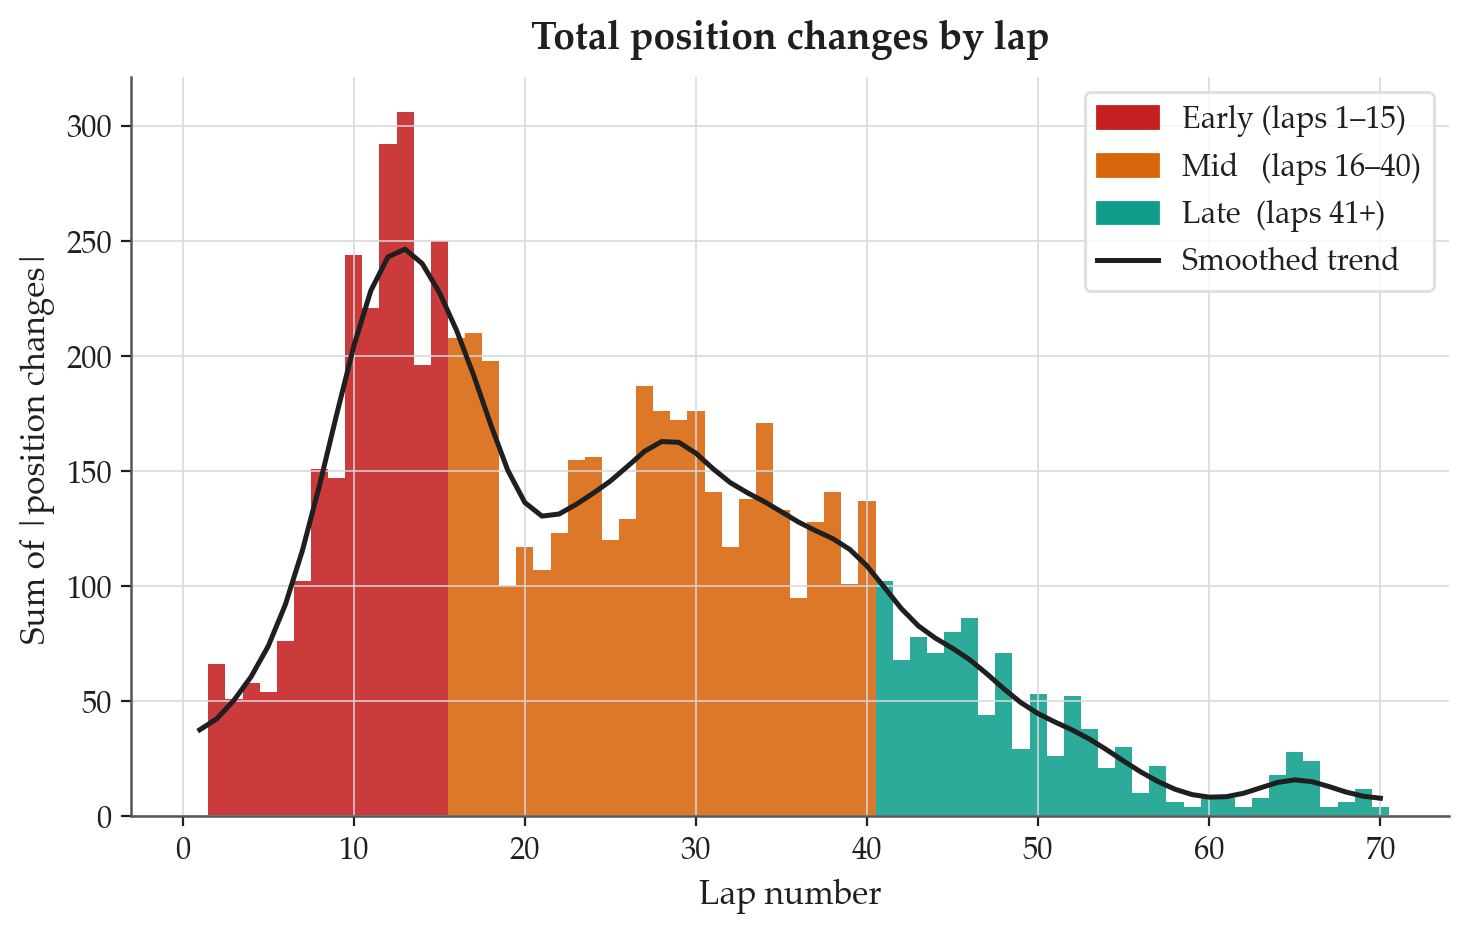
\includegraphics[width=0.82\textwidth]{05a_position_changes.png}
  \caption{Total position changes per lap, $2024$ season aggregated
  across all $23$ races. Early laps (red) and the primary pit
  window (orange) dominate; late-race changes (teal) are sparser.}
  \label{fig:race-pos-changes}
\end{figure}

\begin{figure}[H]
  \centering
  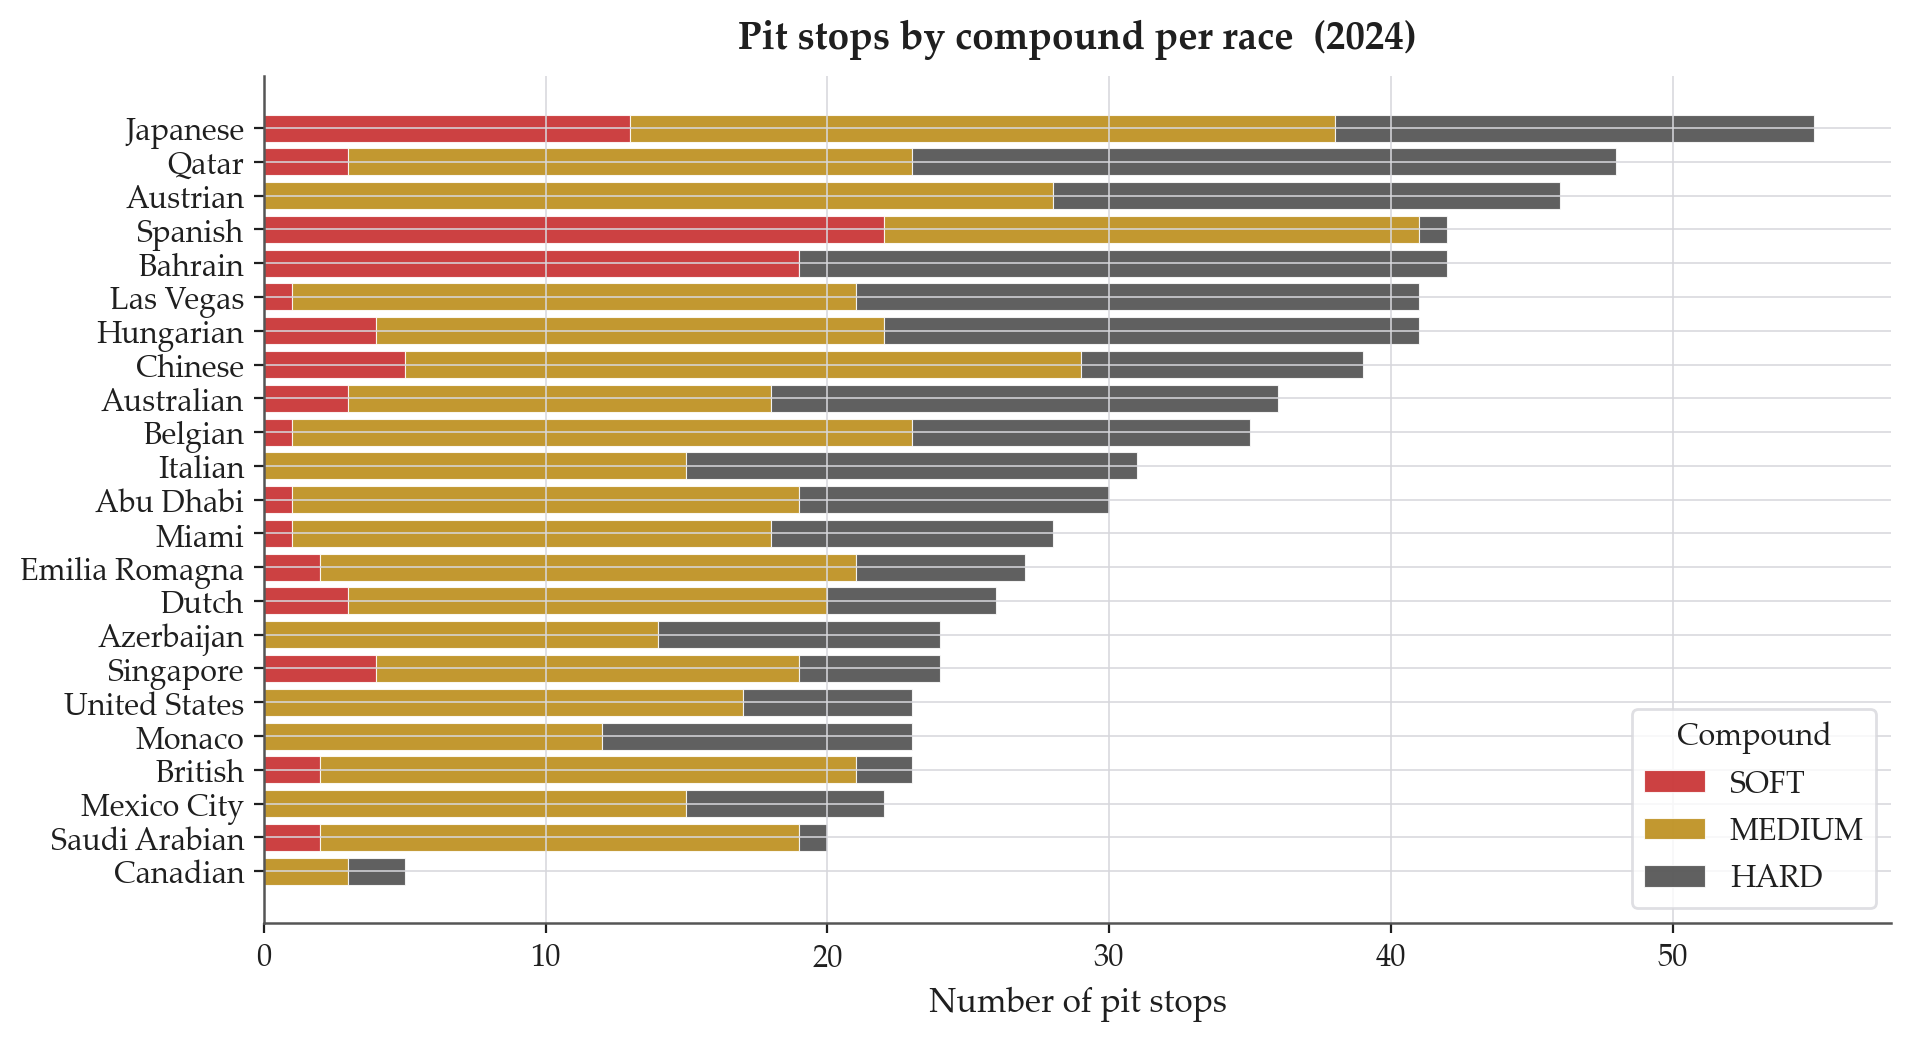
\includegraphics[width=0.92\textwidth]{05c_pit_compound_season.png}
  \caption{Pit-stop counts by tyre compound, per race ($2024$
  season; rows ordered by total pit count). Soft-heavy strategies
  appear at Bahrain, Spain and Japan; the Italian, Belgian and
  Hungarian Grands Prix were essentially Medium--Hard only.}
  \label{fig:race-pit-compound}
\end{figure}

\subsection{Descriptive analytics}
Population-level descriptive statistics for the $2024$ subset are
collected in Table~\ref{tab:pit-desc}. The primary pit window centres
on lap $\sim 25$, with mean tyre life at pit $\sim 18$ laps.

\begin{table}[H]
  \centering
  \caption{Population-level descriptive statistics, 2024 season.}
  \label{tab:pit-desc}
  \begin{tabular}{ll}
    \toprule
    Quantity & Value \\
    \midrule
    Mean lap time                  & $92.8$ s \\
    Mean pit lap                   & $24.9$ \\
    Mean tyre life at pit          & $18.2$ laps \\
    Pit-stop positive rate         & $3.03\%$ ($731$/$24{,}138$) \\
    \bottomrule
  \end{tabular}
\end{table}

\begin{figure}[H]
  \centering
  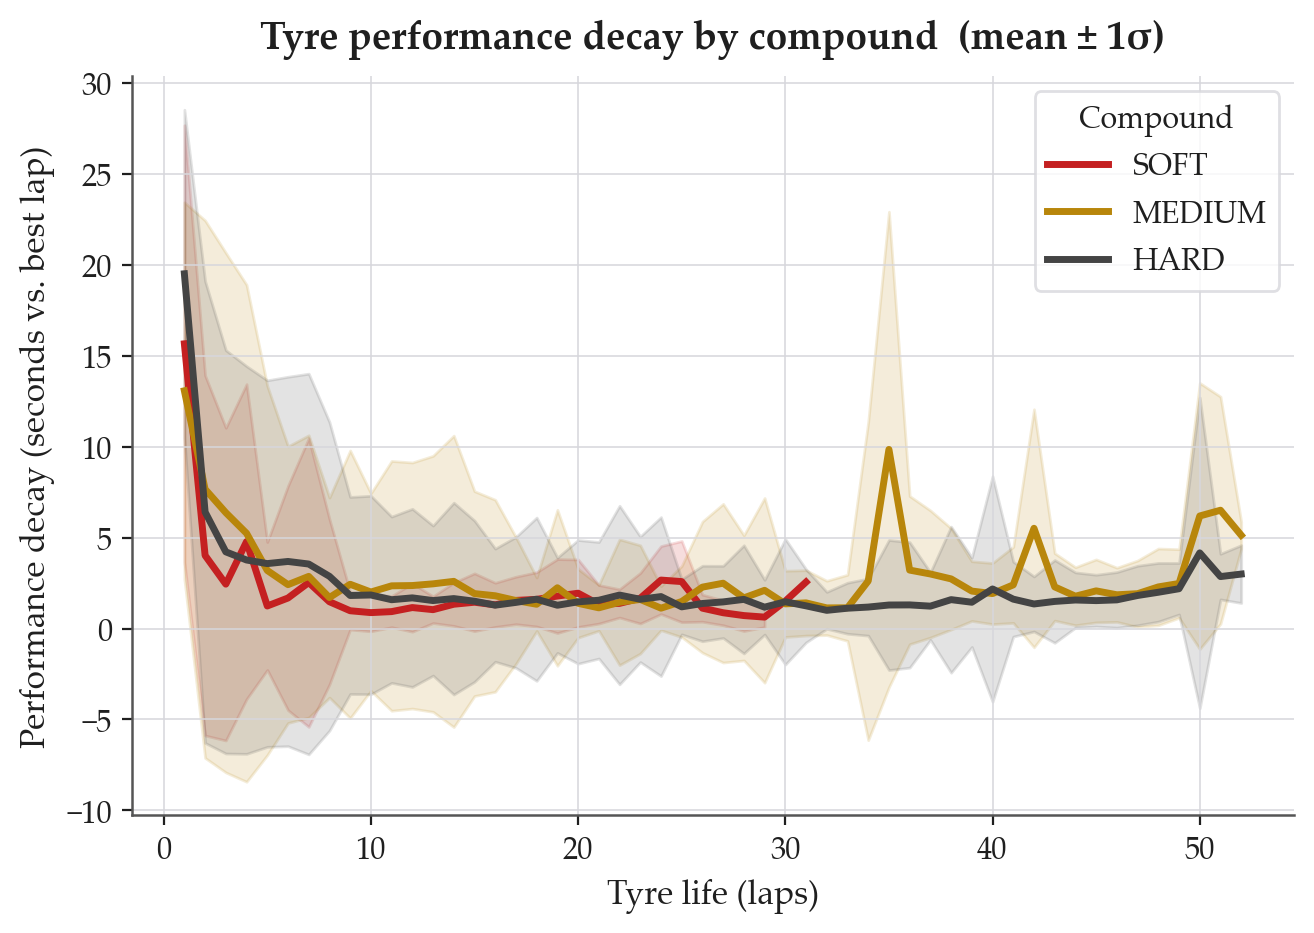
\includegraphics[width=0.82\textwidth]{02a_tyre_decay_compound.png}
  \caption{Compound-specific tyre degradation curves: mean
  performance loss (seconds vs.\ best lap) as a function of tyre age,
  with $\pm 1\sigma$ band. The Soft compound shows the steepest
  cliff.}
  \label{fig:pit-tyre}
\end{figure}

\begin{figure}[H]
  \centering
  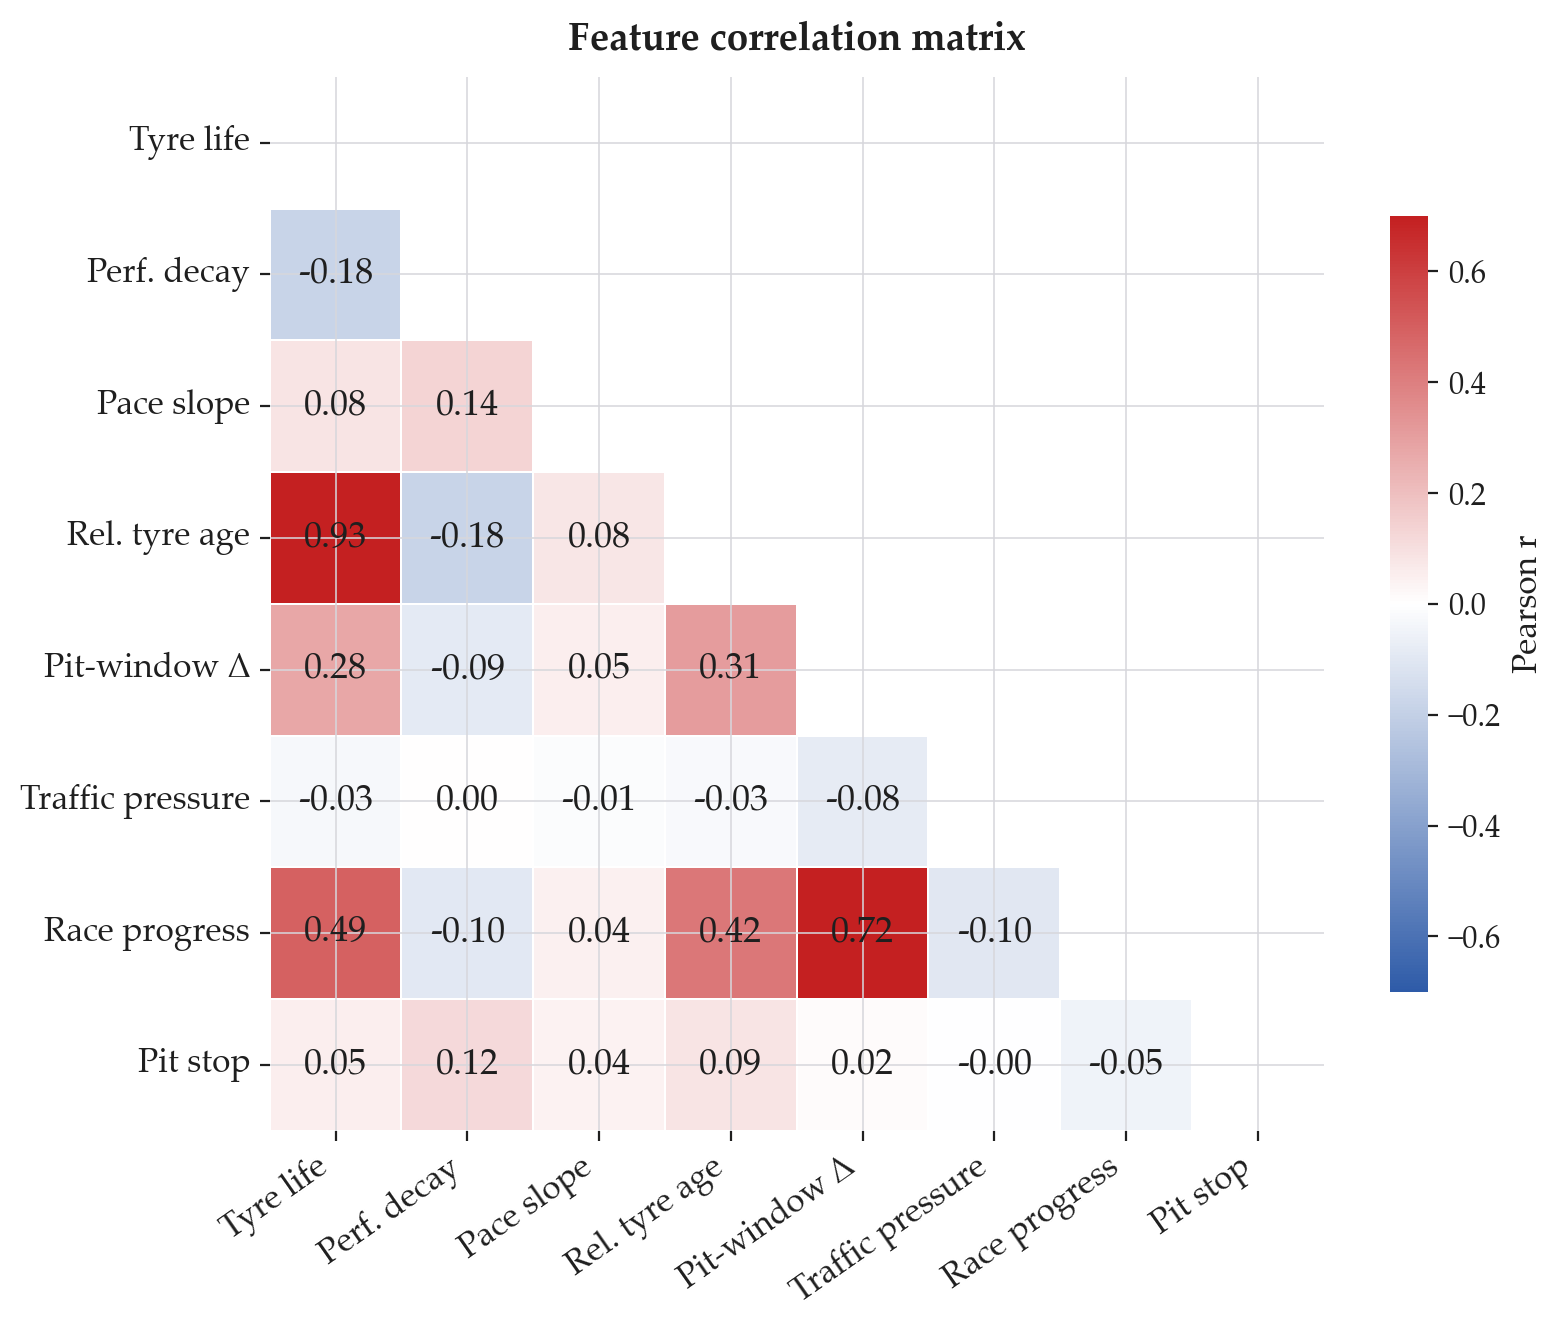
\includegraphics[width=0.82\textwidth]{06a_corr_matrix.png}
  \caption{Pearson correlation between the engineered features
  (lower triangle). The strongest interactions are
  race-progress$\leftrightarrow$pit-window-$\Delta$ ($r=0.72$) and
  race-progress$\leftrightarrow$tyre-life ($r=0.49$); raw
  correlations with the pit-stop indicator are individually small,
  consistent with the BiLSTM's role being to learn the
  non-linear interaction structure rather than to amplify any
  single feature.}
  \label{fig:pit-corr}
\end{figure}

\begin{figure}[H]
  \centering
  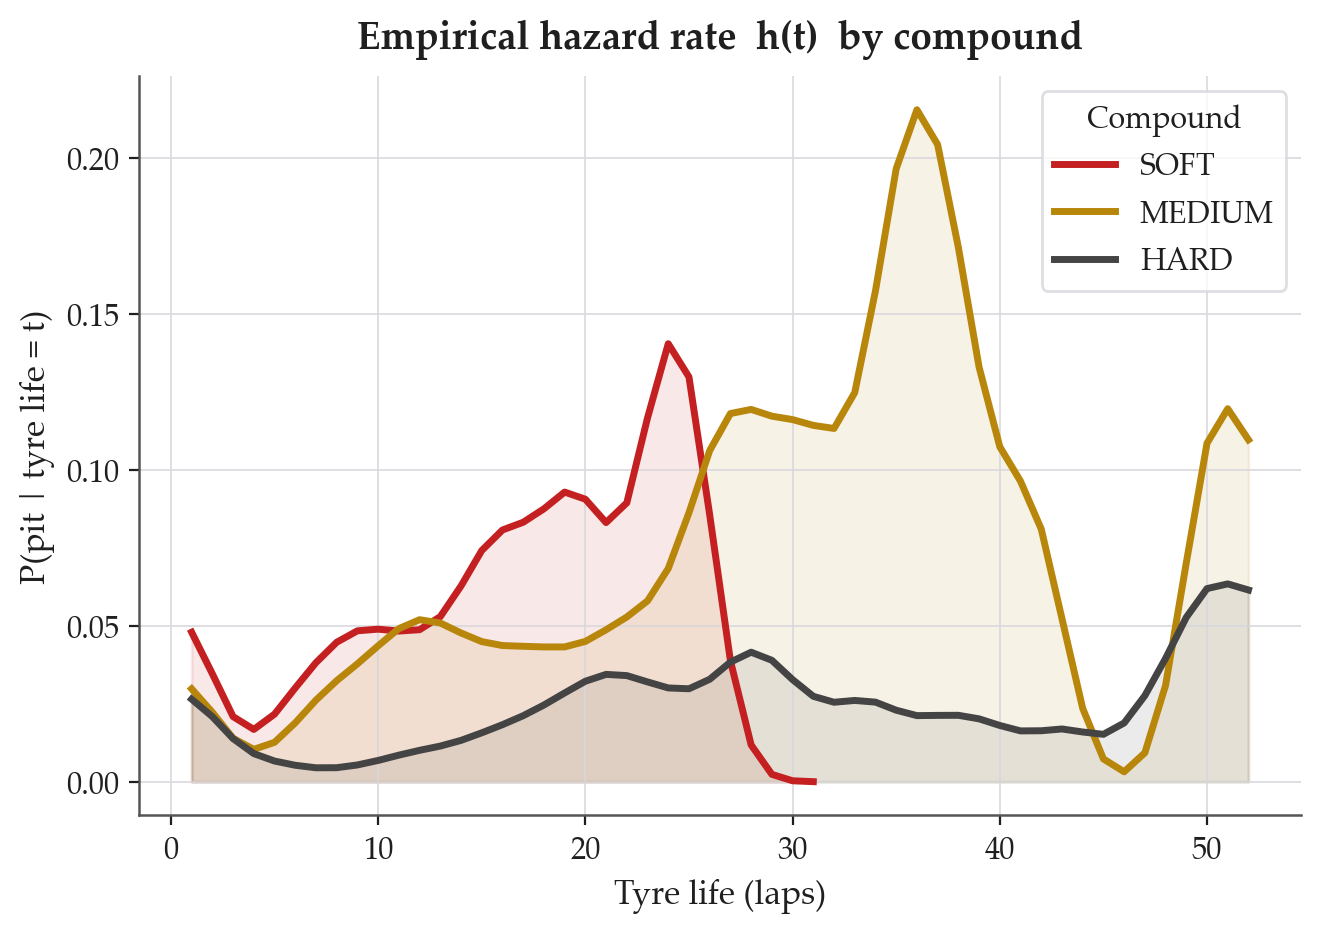
\includegraphics[width=0.82\textwidth]{07a_hazard_rate.png}
  \caption{Empirical pit-hazard rate $h(t)$ as a function of tyre
  age, separated by compound. The Soft hazard rises earliest; the
  Hard much later.}
  \label{fig:pit-hazard}
\end{figure}

\begin{figure}[H]
  \centering
  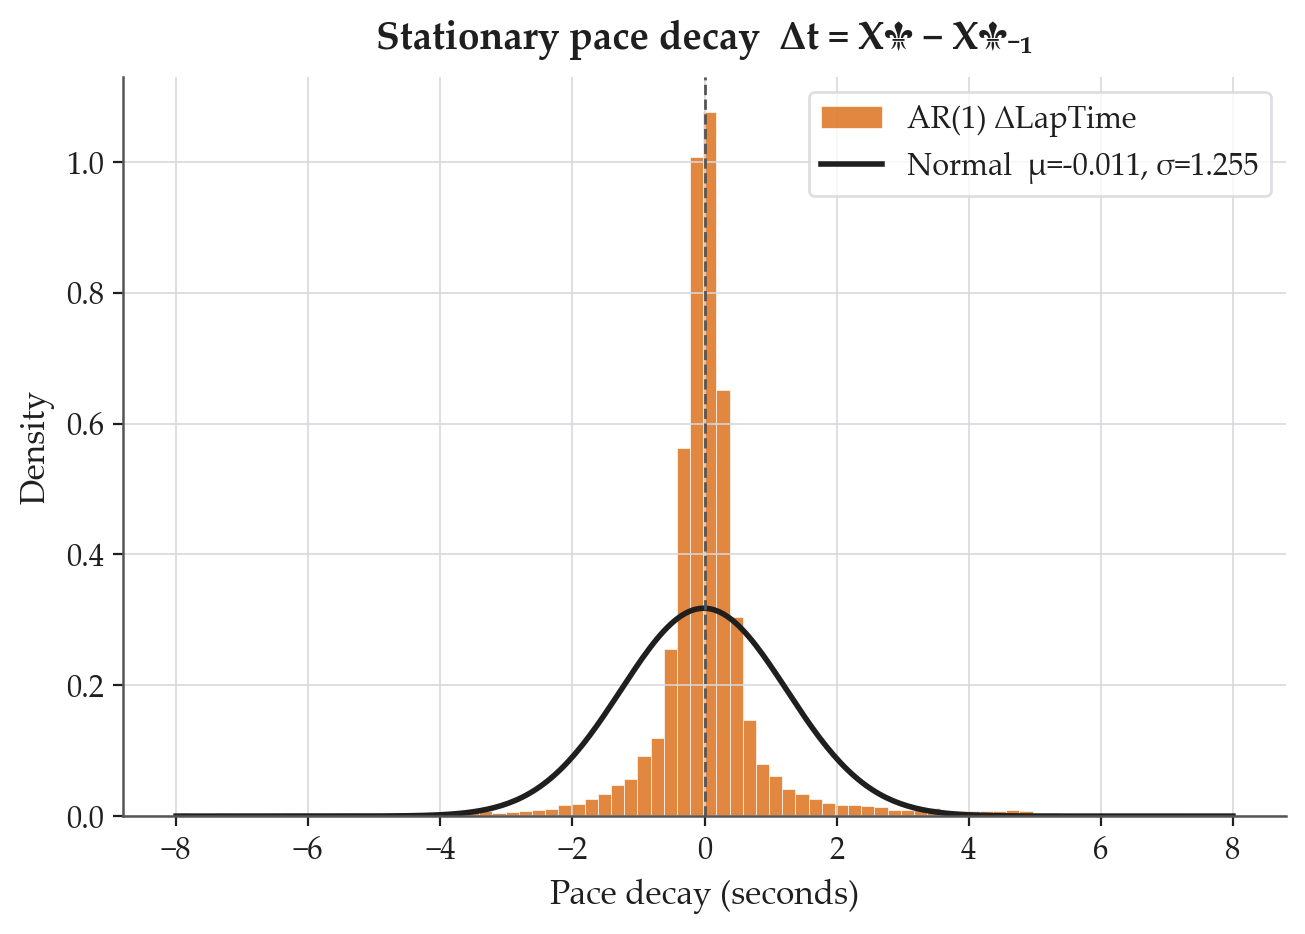
\includegraphics[width=0.82\textwidth]{07b_pace_decay_hist.png}
  \caption{Stationary pace-decay $\Delta X_t = X_t - X_{t-1}$ after
  AR(1) filtering, with a Gaussian fit overlaid. The residuals are
  approximately symmetric around zero, validating the filter.}
  \label{fig:pit-pacedecay}
\end{figure}

\subsection{Discussion and future directions}
The BiLSTM is operationally useful: on true pit laps in $2025$ it
assigns mean probability $84\%$, against a near-zero baseline on
non-pit laps. The Cox model gives a complementary, interpretable
hazard baseline that the deep model can be stacked against. Team
profiles partition naturally into deterministic and opportunistic
strategy cultures. The full pipeline --- predicted pit probability,
overtake classification, VSC agility score --- supplies the building
blocks for race-time strategic decision support.

A natural set of extensions follows.
\begin{itemize}
  \item \textbf{Attention.} Replacing the BiLSTM stack with a small
  self-attention encoder would expose, lap-by-lap, which historical
  laps the model is conditioning on. Attention weights are far easier
  to debug than recurrent hidden states.
  \item \textbf{Multi-task heads.} A single backbone could
  simultaneously predict the binary pit indicator, the tyre-compound
  choice, and the residual stint length. Joint training tends to
  regularise each head.
  \item \textbf{Calibration.} Raw sigmoid outputs are not calibrated
  probabilities. Platt scaling or isotonic regression on the held-out
  season would yield probabilities that match empirical pit-stop
  frequencies, a prerequisite for use inside a strategy simulator.
  \item \textbf{Weather.} The single largest unmodelled covariate.
  Rain probability and track temperature reshape every part of the
  pit decision and would be the first feature to add in a richer
  pipeline.
\end{itemize}

% =====================================================================
\section{Joint Discussion}\label{sec:joint}
% =====================================================================

The four studies above were performed independently and each used
different statistical machinery. Read together, three cross-cutting
observations stand out.

\paragraph{Machinery first, driver second.}
Sections~\ref{sec:grid}--\ref{sec:home} both demonstrate the
dominance of the car. In Section~\ref{sec:grid}, the constructor
strength index alone explains more variance than any other feature
in the linear regression, and grid position --- itself largely a
consequence of car capability --- comes second. In Section~\ref{sec:home}
the teammate delta exists precisely to subtract the car off; once it
is removed, the apparent home effect vanishes. A naive analysis that
ignores the car will find a ``home effect'' for any driver who
happens to have driven a competitive car at their home Grand Prix,
and will find no effect for any driver who happened not to.

\paragraph{Era drift matters as much as model choice.}
Section~\ref{sec:lap} shows lap times tightening dramatically in the
modern ground-effect era ($\sigma = 0.72$\,s at Monza $2023$ vs.\
$1.44$\,s in $2005$). Section~\ref{sec:home} requires era adjustment
just to make the dependent variable coherent. Section~\ref{sec:pit}
trains and tests across seasons explicitly because the pit-stop
distribution shifts every year with tyre supply, sprint formats, and
DRS rules. In each case, era is not a nuisance to be averaged over;
it is part of the model's data-generating process.

\paragraph{The right baseline beats the right model.}
The pit-stop BiLSTM is more sophisticated than the lap-time MLE
fits, but the operational uplift from each comes from the
\emph{baseline} the model is benchmarked against. A BiLSTM that
beats a Cox proportional-hazards baseline by $\Delta\!\text{AUC-PR}$
points is a stronger claim than one that beats a constant predictor.
Likewise, the home-advantage paired $t$-test would have been
meaningless without first constructing the teammate delta, and the
podium-decay analysis in Section~\ref{sec:grid} would be misleading
without the empirical $P(\text{Win}\mid\text{Pole})=43\%$ anchor.

\paragraph{What we did not do.}
Three obvious omissions cut across the four studies. None of the
analyses incorporate weather --- wet-race outcomes are systematically
different in distribution and would deserve a separate treatment.
None of the analyses model strategic interactions across drivers
(undercut races, blocking) explicitly. And none use FastF1-grade
per-lap telemetry for the pre-$2018$ era, because it does not exist;
the historical studies are therefore based on lower-resolution data
than the modern pit-stop study.

% =====================================================================
\section{Conclusions}\label{sec:concl}
% =====================================================================

Four studies, one substantive thread. The right choice of target
variable does most of the methodological work in each.
\begin{itemize}
  \item For \textbf{lap times}, the right target is the cleaned
  within-race distribution; the right model class is the right-skewed
  families (Gamma, Log-Normal), not the Normal.
  \item For \textbf{grid advantage}, the right target is the
  finishing position controlled for constructor strength; pole
  position remains the single dominant signal.
  \item For \textbf{home advantage}, the right target is the
  era-adjusted teammate delta, which removes both the car and the
  points-system confound; the aggregate home effect is then
  statistically zero, and only a small experience interaction survives.
  \item For \textbf{pit strategy}, the right target is the per-lap
  pit indicator on length-$20$ telemetry windows; a BiLSTM
  recovers an $84\%$ mean probability on true pit laps.
\end{itemize}

The recurring message --- in a sport where machinery and rules drift
faster than driver skill --- is that the modelling choice that
matters most is the one made before any model is fit. The four
analyses converge on this single point from very different
statistical directions.

% =====================================================================
\appendix
\section{Reproducibility}
% =====================================================================

\paragraph{Software.}
All four pipelines run under Python 3.11/3.12. The shared scientific
stack is \code{pandas}, \code{numpy}, \code{scipy},
\code{statsmodels}, \code{scikit-learn}, \code{matplotlib} and
\code{seaborn}. The home-race study additionally uses \code{xgboost}
and \code{shap}; the pit-stop study uses \code{torch},
\code{lifelines}, and (for raw data acquisition only) \code{fastf1};
the grid-position study uses \code{tensorflow} for its LSTM
regressor. Random seeds are fixed to $42$ throughout. For TensorFlow,
\code{tf.config.experimental.enable\_op\_determinism()} forces
deterministic kernels so that the held-out LSTM MAE is exactly
reproducible at $2.87$ positions.

\paragraph{Data.}
The Kaggle Ergast redistribution lives in \code{data/raw/}; a curated
nationality-to-country mapping is shipped as \code{countries.csv}
and used by the home-race study. The pit-stop subproject also requires
per-lap telemetry CSVs from the FastF1 API (several gigabytes), which
are not distributed in the repository because of their size;
pre-trained BiLSTM weights are shipped under
\code{outputs/pit\_stop\_strategy/models/} so that all figures can be
regenerated without retraining.

\paragraph{Entry points.}
From the repository root,
\begin{verbatim}
python -m src.lap_time_distributions.lap_distributions
python -m src.starting_grid_advantage.main
python -m src.home_advantage.run_analysis
python -m src.pit_stop_strategy.visualize
\end{verbatim}
each regenerate the artefacts under the corresponding
\code{outputs/} subdirectory. Per-subproject \code{README.md} files
document the full multi-stage commands where applicable.

\end{document}
